%%% DOCUMENTCLASS 
%%%-------------------------------------------------------------------------------

\documentclass[
a6paper, % Stock and paper size.
11pt, % Type size.
% article,
% oneside, 
onecolumn, % Only one column of text on a page.
% openright, % Each chapter will start on a recto page.
% openleft, % Each chapter will start on a verso page.
openany, % A chapter may start on either a recto or verso page.
]{memoir}

%%% PACKAGES 
%%%------------------------------------------------------------------------------

\usepackage[utf8]{inputenc} % If utf8 encoding
% \usepackage[lantin1]{inputenc} % If not utf8 encoding, then this is probably the way to go
\usepackage[T1]{fontenc}    %
\usepackage[ngerman]{babel} % English please
\usepackage{eurosym}
\usepackage[final]{microtype} % Less badboxes

\usepackage[pass,a6paper]{geometry}

% \usepackage{kpfonts} %Font
\usepackage[euler-digits]{eulervm} % Math Font
\usepackage{gensymb} % Text Symbols
\usepackage{amsmath,amssymb,mathtools} % Math
\usepackage{nicefrac}
% \usepackage{empheq}
%  German Math Punctuation
\DeclareMathSymbol{,}{\mathpunct}{letters}{"3B}
\DeclareMathSymbol{.}{\mathord}{letters}{"3B}
\DeclareMathSymbol{\decimal}{\mathord}{letters}{"3A}
% Typesetting Theorems
\allowdisplaybreaks
\usepackage[amsmath,thmmarks,hyperref,thref]{ntheorem}


\theoremstyle{break}
\theorembodyfont{\upshape}
% \theoremsymbol{\ensuremath{\diamondsuit}}
\newtheorem{defi}{Definition}

% \renewcommand{\thedefi}{\arabic{defi}}
\theoremstyle{break}
\theoremsymbol{}
\newtheorem{beme}[defi]{Bemerkung}

\theorembodyfont{\itshape}
% \theoremsymbol{\ensuremath{\triangledown}}
\newtheorem{satz}[defi]{Satz}
\newtheorem{lemm}[defi]{Lemma}
\newtheorem{folg}[defi]{Folgerung}

\theorembodyfont{\upshape}
% \theoremsymbol{\ensuremath{\bigstar}}
% \theoremseparator{:}
\newtheorem{regel}[defi]{Regel}

\theoremstyle{changebreak}
\theorembodyfont{\itshape}
\theoremprework{\bigskip\begin{center}
 \includegraphics[width=.5\textwidth]{./Vintage-Decorative-Divider.pdf}
 % Vintage-Decorative-Divider.pdf: 0x0 pixel, 300dpi, 0.00x0.00 cm, bb=
\end{center}}
\newtheorem{ssatz}[defi]{Satz}

\theoremprework{}
\theorempostwork{}
\theoremstyle{nonumberbreak}
\theorembodyfont{\upshape}
% \theoremsymbol{\ensuremath{\ast}}
\newtheorem{bsp}{Beispiel}
\theoremstyle{nonumberplain}
\theoremheaderfont{\itshape}
\theoremsymbol{\ensuremath{\square}}
\theoremseparator{}
\theorempostwork{\begin{center}
 \includegraphics[width=.5\textwidth]{./Vintage-Decorative-Divider.pdf}
 % Vintage-Decorative-Divider.pdf: 0x0 pixel, 300dpi, 0.00x0.00 cm, bb=
\end{center}\bigskip}
\newtheorem{bew}{\framebox{Beweis}}

\usepackage{epigraph} % Quotation at the beginning of parts / chapters

\usepackage{tikz, pgfplots} % Figures
\usetikzlibrary{fit}
\usepackage{tkz-euclide}
\usetkzobj{all}
\usepackage{graphicx} % Include figures

% framing equations
\usetikzlibrary{shadows} %defines shadows
\usetikzlibrary{decorations.text}
\usepackage[framemethod=tikz]{mdframed} % frame defining
\global\mdfdefinestyle{myboxstyle}{%
shadow=true,
linecolor=black,
shadowcolor=black,
shadowsize=6pt,
nobreak=false,
innertopmargin=10pt,
innerbottommargin=10pt,
leftmargin=5pt,
rightmargin=5pt,
needspace=1cm,
skipabove=5pt,
skipbelow=10pt,
middlelinewidth=1pt,
afterlastframe={\vspace{5pt}},
aftersingleframe={\vspace{5pt}},
tikzsetting={%
draw=black,
thick}
}
% breakable box
\newmdenv[style=myboxstyle]{whitebox}
% unbreakable box
\newmdenv[style=myboxstyle,nobreak=true]{blockwhitebox}


%%% PAGE LAYOUT 
%%%------------------------------------------------------------------------------

\setlrmarginsandblock{0.075\paperwidth}{*}{1} % Left and right margin
\setulmarginsandblock{0.15\paperwidth}{*}{1}  % Upper and lower margin
\checkandfixthelayout

%%% SECTIONAL DIVISIONS
%%%------------------------------------------------------------------------------

\maxsecnumdepth{subsection} % Subsections (and higher) are numbered
\setsecnumdepth{subsection}

\makeatletter %
\makechapterstyle{standard}{
  \setlength{\beforechapskip}{0\baselineskip}
  \setlength{\midchapskip}{1\baselineskip}
  \setlength{\afterchapskip}{4\baselineskip}
  \renewcommand{\chapterheadstart}{\vspace*{\beforechapskip}}
  \renewcommand{\chapnamefont}{\normalfont\Large}
  \renewcommand{\printchaptername}{\chapnamefont \@chapapp}
  \renewcommand{\chapternamenum}{\space}
  \renewcommand{\chapnumfont}{\normalfont\Large}
  \renewcommand{\printchapternum}{\chapnumfont \thechapter}
  \renewcommand{\afterchapternum}{\par\nobreak\vskip \midchapskip}
  \renewcommand{\printchapternonum}{\vspace*{\midchapskip}\vspace*{5mm}}
  \renewcommand{\chaptitlefont}{\bfseries\LARGE}
  \renewcommand{\printchaptertitle}[1]{\chaptitlefont ##1}
  \renewcommand{\afterchaptertitle}{\par\nobreak\vskip \afterchapskip}
}
\setlength{\epigraphwidth}{0.5\textwidth}
\makeatother

\chapterstyle{standard}

\setsecheadstyle{\normalfont\large\bfseries}
\setsubsecheadstyle{\normalfont\normalsize\bfseries}
\setparaheadstyle{\normalfont\normalsize\bfseries}
\setparaindent{0pt}\setafterparaskip{0pt}

%%% FLOATS AND CAPTIONS
%%%------------------------------------------------------------------------------

\makeatletter                  % You do not need to write [htpb] all the time
\renewcommand\fps@figure{htbp} %
\renewcommand\fps@table{htbp}  %
\makeatother                   %

\captiondelim{\space } % A space between caption name and text
\captionnamefont{\small\bfseries} % Font of the caption name
\captiontitlefont{\small\normalfont} % Font of the caption text

\changecaptionwidth          % Change the width of the caption
\captionwidth{1\textwidth} %

%%% ABSTRACT
%%%------------------------------------------------------------------------------

\renewcommand{\abstractnamefont}{\normalfont\small\bfseries} % Font of abstract title
\setlength{\absleftindent}{0.1\textwidth} % Width of abstract
\setlength{\absrightindent}{\absleftindent}

%%% HEADER AND FOOTER 
%%%------------------------------------------------------------------------------

\makepagestyle{standard} % Make standard pagestyle

\makeatletter                 % Define standard pagestyle
\makeevenfoot{standard}{}{}{} %
\makeoddfoot{standard}{}{}{}  %
\makeevenhead{standard}{\small\rightmark}{}{\itshape\thepage}
\makeoddhead{standard}{\small\rightmark}{}{\itshape\thepage}
% \makeoddhead{standard}{}{}{\small\rightmark\qquad\bfseries\thepage}
\makeheadrule{standard}{\textwidth}{\normalrulethickness}
\makeatother                  %

\makeatletter
\makepsmarks{standard}{
\createmark{chapter}{both}{shownumber}{\@chapapp\ }{ \quad }
\createmark{section}{both}{shownumber}{}{ \quad }
\createplainmark{toc}{both}{\contentsname}
\createplainmark{lof}{both}{\listfigurename}
\createplainmark{lot}{both}{\listtablename}
\createplainmark{bib}{both}{\bibname}
\createplainmark{index}{both}{\indexname}
\createplainmark{glossary}{both}{\glossaryname}
}
\makeatother                               %

\makepagestyle{chap} % Make new chapter pagestyle

\makeatletter
\makeevenfoot{chap}{}{\small\thepage}{} % Define new chapter pagestyle
\makeoddfoot{chap}{}{\small\thepage}{}  %
\makeevenhead{chap}{}{}{}   %
\makeoddhead{chap}{}{}{}    %
% \makeheadrule{chap}{\textwidth}{\normalrulethickness}
\makeatother

\nouppercaseheads
\pagestyle{standard}               % Choosing pagestyle and chapter pagestyle
\aliaspagestyle{chapter}{chap} %

%%% NEW COMMANDS
%%%------------------------------------------------------------------------------

\newcommand{\p}{\partial} %Partial
% Or what ever you want

\def\fc{(0,0) circle (1.5cm)}
\def\sc{(0:2cm) circle (1.5cm)}

%%% TABLE OF CONTENTS
%%%------------------------------------------------------------------------------

\maxtocdepth{subsection} % Only parts, chapters and sections in the table of contents
\settocdepth{subsection}

\AtEndDocument{\addtocontents{toc}{\par}} % Add a \par to the end of the TOC

%%% INTERNAL HYPERLINKS
%%%-------------------------------------------------------------------------------

\usepackage{hyperref}   % Internal hyperlinks
\hypersetup{
pdfborder={0 0 0},      % No borders around internal hyperlinks
pdfauthor={Martin Putzlocher} % author
}
\usepackage{memhfixc}   %

%%% THE DOCUMENT
%%% Where all the important stuff is included!
%%%-------------------------------------------------------------------------------

\author{Martin Putzlocher}
\title{Mathematik\\in der\\9.~Jahrgangsstufe\\~\\{\small Gymnasium Bayern}}

% \usepackage{lipsum} % Just to put in some text

\begin{document}

\frontmatter

\maketitle
\newpage
\null\vfill

\begin{flushleft}
\textcopyright COPYRIGHT INFO

\textit{Mathematik in der 9.~Jahrgangsstufe}

2017

von Martin Putzlocher, Wiesau

Studienrat am Stiftland-Gymnasium in Tirschenreuth, Bayern
\bigskip

 \includegraphics[height=2em]{./cc88x31.png}
 
Dieses Werk ist lizenziert unter einer Creative Commons Namensnennung - \textbf{Nicht-kommerziell} - Weitergabe unter gleichen Bedingungen 4.0 International Lizenz.
Die Nutzung an Privatschulen, kirchlichen Schulen oder Nachhilfeinstituten ist nicht gestattet.

Der Urheber aller Abbildungen ist, wenn nicht anders vermerkt, der Autor.
\end{flushleft}
\clearpage


% \begin{abstract}
% \lipsum[1-2]
% \end{abstract}
% \clearpage

\tableofcontents*
\clearpage

\chapter{Einleitung}
Dieses elektronische Buch soll Schülerinnen und Schülern in der 9.~Jahrgangsstufe des Gymnasiums in Bayern oder Lernenden, die einem vergleichbaren Anforderungsniveau gegenüber stehen, helfen, sich im undurchschaubaren Dickicht mathematischer Ausdrücke zurechtzufinden.

\mainmatter


\part{Grundwissen im Vorfeld der 9.~Jahrgangsstufe}


\chapter{Algebra und Analysis bis zur 9.~Jahrgangsstufe}
\label{ch:grundwissen}
\epigraph{Die Neugier steht immer an erster Stelle eines Problems, das gelöst werden will.}{\textsc{Galileo Galiei}}


Nachfolgend werden alle Rechenregeln und Definitionen algebraischer Strukturen wiedergegeben, die bis zum Beginn der 9.~Jahrgangsstufe am Gymnasium in Bayern erlernt werden sollen. Dabei wird darauf geachtet, dass die Notation mit dem heutigen Standard in der Mathematik übereinstimmt.

\section{Zahlen}

Folgende Zahlenmengen sollten zu Beginn der 9.~Jahrgangsstufe vertraut sein:
\begin{itemize}
 \item \(\mathbb{N}\), die \emph{natürlichen} Zahlen. Das sind die Zahlen, mit denen man abzählt.\\
       \(\mathbb{N}=\lbrace 1;2;3;4;\ldots\rbrace\).
       Jede natürliche Zahl \(n\) hat einen Nachfolger \(n+1\).\footnote{Axiom vom \emph{Nachfolger}}
 \item \(\mathbb{N}_0\), die natürlichen Zahlen mit der Zahl \(0\).\\
 Die grafische Darstellung entspricht den Zahlen am Zahlenstrahl, der mit der \(0\) beginnt
 \item \(\mathbb{Z} = \mathbb{N}\cup \lbrace 0\rbrace \cup{}-\mathbb{N}\), die \emph{ganzen} Zahlen.\\
 Die grafische Darstellung entspricht den Zahlen an der Zahlengeraden.
 \item \(\mathbb{Q}\), die \emph{rationalen Zahlen}. Das sind alle Zahlen, die man als Bruch schreiben kann.\\
       \(\mathbb{Q} = \left\lbrace \frac{p}{q} \mid p\in\mathbb{Z}\;\text{und}\; q\in\mathbb{N}\right\rbrace\)\\
 Die grafische Darstellung der rationalen Zahlen entspricht der Zahlengeraden.
\end{itemize}

\begin{defi}[Teilbarkeit]
 Eine ganze Zahl \(a\) ist durch eine ganze Zahl \(b\) (ohne Rest) \emph{teilbar}, wenn \(a\) ein Vielfaches von \(b\) ist.\index{teilbar} Man sagt dann auch, "`\(b\) teilt \(a\)"' oder in Symbolen:
 \begin{equation*}
  b\mid a \Leftrightarrow a = k\cdot b\;\text{mit}\;k\in\mathbb{Z}
 \end{equation*}
\end{defi}

\begin{bsp}[Teilbarkeit]
 124 ist durch 4 teilbar oder in Zeichen \\\(4 \mid 124\), da \(124 = 31 \cdot 4\).
\end{bsp}


\begin{defi}[teilerfremd]
 Zwei ganze Zahlen \(a\) und \(b\) nennt man \emph{teilerfremd}, wenn es außer der Zahl \(1\) keine andere Zahl gibt, durch die beide teilbar sind.\index{teilerfremd}
\end{defi}

\begin{bsp}[teilerfremd]
 23 und 24 sind teilerfremd, da sie außer 1 keine gemeinsamen Teiler besitzen.
 
 123 und 39 sind nicht teilerfremd, da beide Zahlen durch 3 teilbar sind.
\end{bsp}

\begin{defi}[Primzahl]
Primzahlen sind die natürlichen Zahlen, die nur durch 1 und sich selbst teilbar sind.\index{Primzahl}
\end{defi}
\begin{folg}
Jede natürliche Zahl lässt sich als Produkt von Primzahlen schreiben. Dieses Produkt nennt man die \emph{Primfaktorzerlegung} dieser Zahl.\index{Primfaktorzerlegung}
\end{folg}
\begin{bsp}
 \begin{equation*}
  312 = 3\cdot 104 = 3\cdot 2 \cdot 52 = 3\cdot 2 \cdot 2 \cdot 26 = 3\cdot 2\cdot 2 \cdot 2 \cdot 13
 \end{equation*} 
\end{bsp}

\begin{defi}[Primfaktoren]
 Jede natürliche Zahl, die größer als 1 und selbst keine Primzahl ist, lässt sich als Produkt von mindestens zwei Primzahlen schreiben, die dann als \emph{Primfaktoren} bezeichnet werden.\index{Primfaktor}
 \begin{equation*}
  n = p_1 \cdot p_2 \cdot p_3 \cdots
 \end{equation*}
 Der Prozess zur Bestimmung dieser Primzahlen nennt man die \emph{Primfaktorzerlegung}. Die leichteste Methode hierfür ist die Probedivision. Dabei prüft man, ausgehend von der \(2\), der Reihe nach, welche Primzahl die zu zerlegende Zahl ohne Rest teilt. Hat man einen solchen Teiler gefunden, führt man die Division aus und wiederholt das Verfahren am Ergebnis der Division. Prüft man hierbei einen möglichen Teiler, der bereits größer als die Quadratwurzel\footnote{siehe Stoff der 9.~Jahrgangsstufe} der zu untersuchenden Zahl ist, kann man das Verfahren abbrechen: Die Zahl ist dann selbst eine Primzahl.
\end{defi}

\begin{bsp}
 Primfaktorzerlegung der Zahl 315
 \begin{align*}
  2 &\nmid 315 \\
  3 &\mid 315  & 315 \div 3 &= 105\\
  3 &\mid 105  & 105 \div 3 &= 35\\
  3 &\nmid 35  \\
  5 &\mid 35 &  35 \div 5 &= 7 \\
  7 &\;\text{ist prim}\\ \hline
  315 &= 3\cdot 3 \cdot 5 \cdot 7
 \end{align*}

\end{bsp}

\section{Größen}
\label{sec:groessen}
\begin{defi}[Größe]
 Eine \emph{Größe} ist ein Ergebnis einer Messung anhand einer Skala mit vorher festgelegter Einheit.\index{Größe} Die Angabe einer Größe besteht immer aus der Angabe des Zahlenwerts \emph{und} der Einheit. Der Wert gibt an, wie oft die Einheit in den Messwert hineinpasst.\index{Einheit}
 \begin{equation*}
  \text{Größe} = \text{Wert} \cdot \text{Einheit}
 \end{equation*}
 In allen Wissenschaften werden Größen mit \emph{Größensymbolen} abgekürzt, die wie Variablen behandelt werden können.
 
 Achte darauf, Größensymbole und Einheiten nicht zu verwechseln!
\end{defi}

\begin{bsp}[Größen]
 Angaben von Größen sind:
 \begin{align*}
  l &= 3\,\text{m}&&\text{Länge}\\
  \vartheta &= 21\,\degree\text{C}&&\text{Temperatur}\\
  I &= 2.4\,\text{A}&&\text{Stromstärke}\\
  U&= 5\,\text{V}&&\text{elektrische Spannung}\\
  m &= 79\,\text{kg}&&\text{Masse}
 \end{align*}
 Stets lässt sich anhand der Einheit ablesen, um welche Art von Größe\footnote{Statt \emph{Art einer Größe} spricht man auch von ihrer \emph{Dimension}.} es sich handelt.
\end{bsp}

\begin{beme}[Messen]
 Der Vorgang des Messens einer Größe besteht darin, die Eigenschaft eines Untersuchungsgegenstands mittels eines geeigneten Messinstruments mit der Einheit einer Skala zu vergleichen. Messungen an realen Gegenständen sind \emph{immer} mit einer Ungenauigkeit -- dem \emph{Fehler} der Messung\index{Messfehler} -- behaftet. \emph{Fehler} bedeutet hier nicht unbedingt, dass bei der Messung etwas "`systematisch"' falsch gemacht wurde.
\end{beme}

\section{Grundrechenarten und Schreibweisen}

\begin{defi}[Term]
 Jede Rechnung und jeder Teil einer Rechnung wird mit dem Sammelbegriff \emph{Term} (\(\hat{=}\)(Rechen-)Ausdruck) bezeichnet.\index{Term}
\end{defi}

\begin{defi}[Addition]
 Fügt man eine Zahl zu einer anderen hinzu, so spricht man von einer \emph{Addition}\index{Addition}. Der Term wird als \emph{Summe}\index{Summe} bezeichnet. Das Rechenzeichen ist das Plus. Die erste Zahl nennt man den \emph{1.~Summanden}, die zweite den \emph{2.~Summanden}.
\end{defi}
\begin{defi}[Subtraktion]
 Zieht man von einer Zahl eine andere ab, so spricht man von einer \emph{Subtraktion}\index{Subtraktion}. Der Term wird als \emph{Differenz}\index{Differenz} bezeichnet. Das Rechenzeichen ist das Minus. Die erste Zahl nennt man den \emph{Minuenden}\index{Minuend}, die zweite den \emph{Subtrahenden}\index{Subtrahend}.
\end{defi}
\begin{defi}[Multiplikation]
 Vervielfacht man eine Zahl auf das \(n\)-fache, so spricht man von einer \emph{Multiplikation}\index{Multiplikation}. Der Term wird als \emph{Produkt}\index{Produkt} bezeichnet. Das Rechenzeichen ist der Malpunkt.\footnote{im Englischen Sprachraum wird hier das Symbol \(\times\) benutzt.} Die erste Zahl nennt man den \emph{1.~Faktor}, die zweite Zahl~\(n\) den \emph{2.~Faktor}.\index{Faktor}
\end{defi}
\begin{defi}[Division]
 Teilt man eine Zahl auf \(m\) gleiche Teile auf, so spricht man von einer \emph{Division}\index{Division}. Der Term wird als \emph{Quotient}\index{Quotient} bezeichnet. Das Rechenzeichen ist das Divisionszeichen.\footnote{Im deutschen Schulsystem findet man \(a:b\), während International eher \(a\div b\) zur Anwendung kommt.} Die erste Zahl nennt man den \emph{Dividenden}\index{Dividend}, die zweite Zahl~\(m\) den \emph{Divisor}\index{Divisor}.
\end{defi}

\begin{regel}[Schreibweise Produkt]
Wird das Rechenzeichen weggelassen, so ist fast immer ein Produkt gemeint.
\[ab = a\cdot b\]

Die einzige Ausnahme bilden gemischte Brüche:
\begin{align*}a\frac{b}{c} &= a+\frac{b}{c} = \frac{ac+b}{c}\\
   a\frac{b}{c} &\ne \frac{ab}{c} = \frac{a\cdot b}{c} = a\cdot \frac{b}{c}
\end{align*}
\end{regel}

\begin{regel}[Addition negativer Zahlen]
Die Addition einer negativen Zahl entspricht der Subtraktion ihres Betrags.
\begin{align*}
 a+(-b) &= a-b
\end{align*}

Die Subtraktion einer negativen Zahl entspricht der Addition ihres Betrags.
\begin{align*}
 a-(-b) &= a+b
\end{align*}
\end{regel}

\begin{defi}[Umkehraufgabe]
 Mit der \emph{Umkehraufgabe} ist die Umstellung einer Rechnung gemeint, um den ersten Teil des Terms zu bestimmen. Dazu wird die Reihenfolge der Zahlen umgekehrt und die gegenteilige Rechenart ausgeführt. (\(+\leftrightarrow -\) bzw. \(\cdot \leftrightarrow \div\)).
\end{defi}


\section{Grundlegende Rechenregeln}
\label{sec:basicrules}

\subsection*{Vorrangregeln}

\begin{regel}
 Kommt in einer Rechnung nur eine Rechenart vor, so arbeitet man die Rechnung, so wie man sie liest, also \emph{von links nach rechts}, ab.
\end{regel}

\begin{bsp}

\begin{align*}
 3+45-23+12 &=3+45+(-23)+12 \\
  &= 48 + (-23) + 12 \\
  &= 25+12 \\
  &= 37
\end{align*}

 \begin{center}
 \small
   \begin{tikzpicture}[x=1cm,y=1cm]
\node[circle](a) at (0,0) {$3$};
\node[circle](b) at (2,0) {$45$};
\node[draw=black](p1) at (1,0) {$+$};
\node[circle](c) at (1,-1) {$48$};

\node[circle](d) at (3,-1) {$-23$};
\node[draw=black](p2) at (2,-1) {$+$};
\node[circle](e) at (2,-2) {$25$};

\node[circle](f) at (4,-2) {$12$};
\node[draw=black](p3) at (3,-2) {$+$};
\node[circle](g) at (3,-3) {$37$};

\draw (a)--(p1);
\draw (p1)--(b);
\draw (p1)->(c);
\draw (c)--(p2);
\draw (p2)--(d);
\draw (p2)->(e);
\draw (e)--(p3);
\draw (p3)--(f);
\draw (p3)->(g);

\end{tikzpicture}
\normalsize
 \end{center}

\end{bsp}

\begin{regel}[KlaPPS]
 Die Abkürzung steht für:
 \begin{whitebox}
  \textbf{Kla}mmern vor \textbf{P}otenz vor \textbf{P}unkt vor \textbf{S}trich\index{KlaPPS}
 \end{whitebox}
 Bei jedem Rechenausdruck werden also zuerst die Klammern ausgewertet, dann die Potenzen, dann die Punkt-Rechenarten (Multiplikation und Division) und am Schluss die Strich-Rechenarten (Addition und Subtraktion).
 
 Dabei ist zu beachten, dass es Fälle gibt, in denen die Klammern weggelassen werden können. Diese sind:
 \begin{itemize}
  \item Rechnungen auf einem Bruchstrich gelten immer als eingeklammert.
  \[\frac{3+5}{2} = \frac{(3+5)}{2} = \frac{8}{2} = 4\]
  \item Der Exponent einer Potenz gilt als eingeklammert.
  \[2^{5-3} = 2^{(5-3)} = 2^2 = 4\]
 \end{itemize}
\end{regel}
 
 \begin{regel}[Punkt vor Strich]
 Sind in einer Rechnung keine Potenzen und Klammern vorhanden, so vereinfacht sich die KlaPPS-Regel zu\ldots
 \begin{whitebox}
 \begin{center}
  Punkt vor Strich\index{Punkt vor Strich}
  \end{center}
 \end{whitebox}
 Das bedeutet, dass Multiplikation und Division immer Vorrang vor Addition und Subtraktion haben.

\end{regel}

\begin{bsp}
 Die folgende Rechnung beinhaltet alle Rechenarten der KlaPPS-Regel.
 \begin{align*}
  3+7\cdot 2^{3\cdot 2 - 4} &= 3+7\cdot 2^{(3\cdot 2 -4)}\\
                            &= 3+7\cdot 2^{(6-4)}\\
                            &= 3+7\cdot 2^{2} \\
                            &= 3+7\cdot 4 \\
                            &= 3+28 = 31\\
 \end{align*}
 Hier steht eine Summe, ein Produkt und eine Potenz. Also hat die Potenz Vorrang. Der Exponent der Potenz gilt als eine Klammer. Daher wird dieser zuerst ausgewertet. Innerhalb dieser Klammer hat das Produkt Vorrang vor der Differenz. Die erste Rechnung, die ausgeführt wird, ist also \(3\cdot 2\). Die Rechenoperation, die hier zuletzt ausgeführt wird ist die Summe. 
\end{bsp}

\begin{regel}[Benennung von Termen]
 Die Art eines Terms wird durch die zuletzt auszuführende Rechenoperation bestimmt.
\end{regel}

\begin{bsp}[Benennung von Termen]
\begin{align*}
 2+3\cdot 4 &&& \text{Summe} \\
 (2+3)\cdot 7 &&& \text{Produkt} \\
 2^{4-3} &&& \text{Potenz} \\
 2\cdot 8 \div 12 &&& \text{Quotient} \\
 3+4-(5+3) &&& \text{Differenz}
\end{align*}
\end{bsp}


\subsection*{Assoziativgesetz}
\label{ssec:ass} 

\emph{Assoziieren} bedeutet \emph{in Verbindung setzen}. Bei diesem Rechengesetz geht es um die Beliebigkeit der Auswertungsreihenfolge bei bestimmten Termen.

\begin{center}
%  \includegraphics[height=2em]{./assG.png}
 % assG.png: 0x0 pixel, 300dpi, 0.00x0.00 cm, bb=
 \begin{tikzpicture}[x=1cm,y=1cm]
\node[circle, thick, draw=black](a) at (0,0) {$a$};
\node[circle, thick, draw=black](b) at (1,0) {$b$};
\node[circle, thick, draw=black](c) at (2,-1) {$c$};

\draw (a)--node[](ab){} (b);
\draw (ab) |- (c);

\draw[dashed] (3,-1) -- (3,0);

\node[circle, thick, draw=black](a2) at (4,-1) {$a$};
\node[circle, thick, draw=black](b2) at (5,0) {$b$};
\node[circle, thick, draw=black](c2) at (6,0) {$c$};

\draw (b2)--node[](bc){} (c2);
\draw (a2) -|(bc);
\end{tikzpicture}
\end{center}

Innerhalb von Additionen und Multiplikationen ist es erlaubt, die Reihenfolge der Auswertung beliebig zu wählen. In einem Term der gleichen Rechenart können zwei Summanden oder Faktoren beliebig miteinander verbunden werden.\index{Assoziativgesetz} 

\begin{regel}
 Innerhalb einer Summe aus drei oder mehr Summanden dürfen Klammern beliebig gesetzt und damit die Auswertungsreihenfolge beliebig gewählt werden.
 \[ a+b+c = (a+b)+c = a+(b+c) \]
\end{regel}
\begin{regel}
 Innerhalb eines Produkts aus drei oder mehr Faktoren dürfen Klammern beliebig gesetzt und damit die Auswertungsreihenfolge beliebig gewählt werden.
\[ a\cdot b\cdot c = (a\cdot b) \cdot c = a\cdot (b\cdot c)\]
\end{regel}

Achtung! Bei Subtraktionen und Divisionen gilt das Assoziativgesetz \emph{nicht}.
\begin{align*}
 a-b-c &\ne a-(b-c)\\
 a\div b \div c &\ne a\div (b \div c)
\end{align*}

Das Assoziativgesetz erlaubt es beim Kopfrechnen Rechenvorteile dadurch zu erreichen, dass man eine andere Reihenfolge wählt.

\begin{bsp}[Rechenvorteil durch Reihenfolge]
 \[116 + 47 + 453  = 116 + (47+453) = 116 + 500 = 616\] 
\end{bsp}


\subsection*{Kommutativgesetz}
\label{ssec:komm}

Das Lateinische Wort \emph{commutare} bedeutet \emph{vertauschen.}

\begin{center}
 \begin{tikzpicture}[x=1cm,y=1cm]
\node[circle, thick, draw=black, minimum size=2em](a) at (0,0) {$a$};
\node[circle, thick, draw=black, minimum size=2em](b) at (1.5,0) {$b$};
\draw[->] (a)--node[](ab){} (b);
\node[] at (0.75,-1) {erst $a$, dann $b$};
\draw[dashed] (2.5,-0.5) -- (2.5,0.5);
\node[circle, thick, draw=black, minimum size=2em](b2) at (3.5,0) {$b$};
\node[circle, thick, draw=black, minimum size=2em](a2) at (5,0) {$a$};
\draw[<-] (a2)--node[](ab){} (b2);
\node[] at (4.25,-1) {erst $b$, dann $a$};
\end{tikzpicture}
\end{center}

In Additionen und Multiplikationen ist es erlaubt, die Reihenfolge der Terme zu verändern bzw. Terme zu vertauschen (zu \emph{kommutieren}).\index{Kommutativgesetz}

\begin{regel}
 Innerhalb einer Summe dürfen die Summanden vertauscht werden.
 \[a+b = b+a\]
\end{regel}

\begin{regel}
 Innerhalb eines Produkts dürfen die Faktoren vertauscht werden.
 \[a\cdot b = b \cdot a\]
\end{regel}

Achtung! Bei Differenzen und Quotienten gilt das Kommutativgesetz \emph{nicht}!
\begin{align*}
 a-b &\ne b-a\\
 a\div b &\ne b\div a
\end{align*}
Aber eine Differenz kann als Summe mit einer negativen Zahl geschrieben werden, dann ist das Kommutativgesetz wieder anwendbar:
\begin{align*}
 a-b &= a+(-b) \stackrel{\text{KG}}{=} (-b)+a
\end{align*}
Ein Quotient kann als Produkt mit dem Kehrwert des Divisors geschrieben werden, dann ist das Kommutativgesetz wieder anwendbar:
\begin{align*}
 a\div b &= a\cdot \frac{1}{b} \stackrel{\text{KG}}{=} \frac{1}{b}\cdot a
\end{align*}


\subsection*{Gleichnamige Terme}
Zwei Pruduktterme sind \emph{gleichnamig}, wenn sie die gleichen Variablen in der gleichen Häufigkeit enthalten.\index{gleichnamig}

So sind zum Beispiel die Terme \(2x\) und \(-12x\) gleichnamig; \(0.1xy^2\) und \(0.25xy\) hingegen nicht, da \(xy^2\) das \(y\) zweimal als Faktor enthält.

\begin{regel}
 Summen aus gleichnamigen Produkttermen lassen sich zu einem Term zusammenfassen.
 Potenzen gelten nur dann gleichnamig, wenn die Basis und die Exponenten übereinstimmen.
 \end{regel}

\begin{bsp}
 \begin{align*}
  2+4x-7+12x-3y &= 16x-3y-5 \\
  x^2-2x+4x^2 &= 5x^2 -2x \\
  x^3 - y^2 + xy -2x^3 +2y^2 &= -x^3+y^2 +xy 
 \end{align*}

\end{bsp}


\subsection*{Distributivgesetz}
\label{ssec:dis}

Das lateinische \emph{distribuere} bedeutet \emph{verteilen}.

\begin{center}
 \begin{tikzpicture}[x=1cm,y=1cm]
\node[circle, thick, draw=black, minimum size=2em](a) at (0,1) {$a$};

\node[circle, thick, draw=black, minimum size=2em](b) at (1,0) {$b$};
\node[circle, thick, draw=black, minimum size=2em](c) at (2,0) {$c$};
\draw[red] (b)--(c);
\node[rectangle, draw=red, double, fit=(b)(c)](bc) {};

\draw[->] (a)--(bc);

\draw[dashed] (3,-0.5) -- (3,1.5);

\node[circle, thick, draw=black, minimum size=2em](a2) at (5,1) {$a$};
\node[circle, thick, draw=black, minimum size=2em](b2) at (4,0) {$b$};
\node[circle, thick, draw=black, minimum size=2em](c2) at (6,0) {$c$};
\node[rectangle, draw=red, dashed, fit=(a2)(b2)(c2)](bc2) {};
\draw[->] (a2)--node[near end](a2b2){} (b2);
\draw[->] (a2)--node[near end](a2c2){}(c2);
\draw[red] (a2b2) -- (a2c2);
\end{tikzpicture}
\end{center}

Treten Multiplikation und Addition in einem Term auf, so gilt das \emph{Verteilungsgesetz}.\index{Distributivgesetz}

\begin{regel}
 Besteht in einem Produkt ein Faktor aus einer Summe, so ist der Term identisch zur Summe von Produkten.
 \[a\cdot (b+c) = ab+ac\]
\end{regel}

\begin{regel}
Durch die Anwendung des Distributivgesetzes lässt sich also ein Produkt in eine Summe verwandeln. Dann spricht man vom \emph{Ausmultiplizieren}.

Aber auch umgekehrt lässt sich so eine Summe in ein Produkt verwandeln, wenn alle Summanden einen gemeinsamen Faktor besitzen.
\[ 4a+4b = 4\cdot (a+b)\]

Dann spricht man vom \emph{Ausklammern} oder \emph{Faktorisieren}.\index{Ausklammern}\index{Faktorisieren|see {Ausklammern}}

\begin{whitebox}Die beiden Richtungen des Distributivgesetzes\begin{eqnarray*}
 &\rightarrow & \text{ausmultiplizieren} \\
 a\cdot (b+c)&=& a\cdot b + a\cdot c \\
 \text{ausklammern} &\leftarrow&
\end{eqnarray*}
\end{whitebox}

\end{regel}


\begin{regel}[Verteilung des Divisors]
 Ist eine Summe der Dividend eines Quotienten, so kann auch hier der Divisor auf die Summanden verteilt werden.
 \[(a+b)\div c = a\div c + b \div c\]
\end{regel}

\begin{bsp}
 \begin{align*}
  \underbrace{(48+96)}_{144} \div 12 &= 48\div 12 + 96\div 12 \\
                 &= 4 + 8 = 12
 \end{align*}

\end{bsp}

\begin{regel}[Die Minusklammer]

\end{regel}



\subsection*{Aufgaben}

\nameref{sec:sol1}
\begin{enumerate}
 \item Faktorisiere!
 \begin{enumerate}
  \item \(12a+6b\) 
  \item \(19c+11c\)
 \end{enumerate}

\end{enumerate}

\section{Relative Anteile}

\begin{defi}[Anteil, Bruchteil, Verhältnis]\label{D:Anteil}
 Die drei Begriffe \emph{Anteil}\index{Anteil}, \emph{Bruchteil}\index{Bruchteil} und \emph{Verhältnis}\index{Verhältnis} an bzw. zwischen zwei Größen werden häufig synonym als Bezeichnungen für den Quotienten der beiden Größen verwendet. Dabei sind die Größen, die ins Verhältnis gesetzt werden, stets von der gleichen Art. Sie sind also in der gleichen Einheit angebbar. Rechnet man die Größen in eine gemeinsame Einheit um, so kann man diese kürzen und übrig bleibt ein Wert ohne Einheit, die angibt, wie groß der Anteil der einen an der anderen Größe, dem \emph{Grundwert}\index{Grundwert}, ist.
 
 Genau genommen sind die Begriffe \emph{Anteil} und \emph{Bruchteil} aber nicht gleichbedeutend:
 \begin{itemize}
  \item Der \emph{Anteil} steht tatsächlich für einen Bruch wie \(\nicefrac{1}{9}\).
  \item Der \emph{Bruchteil} wären hingegen die 4 von 36~Personen.
 \end{itemize}

\end{defi}

\begin{bsp}[Anteil]
 Sieben von 28 Schülerinnen und Schülern der Klasse 8c sind Brillenträger. Der Anteil der Brillenträger beträgt also:
 \begin{equation*}
  \frac{7}{28} = \frac{1}{4} = 0.25 = 25\,\%
 \end{equation*}
\end{bsp}

\begin{beme}[Prozentangaben]
 Eine Angabe in Prozent ist \emph{keine} Größe; das Prozentzeichen ist \emph{keine} Einheit. Das Prozentzeichen steht einfach nur für ein Hundertstel.\index{Prozent}
 \begin{equation*}
  1\,\% = \nicefrac{1}{100} = \frac{1}{100} = 0.01
 \end{equation*}
 
 Der prozentuale Anteil oder \emph{Prozentsatz}~\(p\) ist der Quotient aus \emph{Prozentwert}~\(P\) und \emph{Grundwert}~\(G\).
 \begin{equation*}
  p = \frac{P}{G}
 \end{equation*}

\end{beme}

\begin{bsp}[Prozentangabe]
Im Jahr 2016 verdienten Frauen im Schnitt \(21\,\%\) weniger als Männer. Der Bruttostundenverdienst von Männern lag bei \(20.71\,\geneuro\).
 
 Der Unterschied im Bruttoverdienst pro Stunde beträgt also \(21\,\%\) von \(20.71\,\geneuro\).
 \begin{equation*}
  P = p \cdot G = 21\,\% \cdot 20.71\,\geneuro = 0.21\cdot 20.71\,\geneuro \approx 4.35\,\geneuro 
 \end{equation*}
 Im Durchschnitt verdienten also Frauen \(4.35\,\geneuro\) weniger pro Stunde.
\end{bsp}

\begin{defi}[Prozentpunkte]
 Bei Änderungen des Prozentsatzes wird häufig nur auf die Änderung der Prozentzahl Bezug genommen. Die Änderung dieses Zahlenwerts wird in \emph{Prozentpunkten} angegeben.
 
 Verringert sich das Wahlergebnis einer Partei von \(22\,\%\) auf \(17\,\%\), so hat sich das Wahlergebnis um \(5\)~Prozentpunkte verschlechtert.
\end{defi}


\begin{regel}[Prozentualer Zuwachs]
 Nimmt eine Größe um einen Prozentsatz~\(p\) zu, so kommt dieser zu den \(100\,\%\) des Grundwerts hinzu. Der Prozentwert wird also zum Grundwert addiert.\index{Zuwachs!prozentualer}
 \begin{equation*}
  G' = G + P = G + p\cdot G = G\cdot (1+p)
 \end{equation*}
 Zinsen auf ein Guthaben sind eine Anwendung des prozentualen Zuwachses. Der Zinssatz ist dabei gleichbedeutend mit dem Prozentsatz~\(p\).
 \end{regel}
 
Häufig ist es in Anwendungen so, dass der Wert nach dem prozentualen Zuwachs als neuer Grundwert erneut Zuwachs erhält. (Zinseszins-Effekt)

\begin{bsp}[Zinseszins]
 Hans legt bei der Reibeisenbank \(1000\,\geneuro\) zu \(2\,\%\) Zinsen p.a.\footnote{p.a. steht für lateinisch \emph{per annum}, also \emph{pro Jahr}.} an. Auf welchen Betrag ist seine Anlage nach vier Jahren angewachsen?\index{Zinseszins}
 
 Das Kapital am Anfang wird als \(K_0\) bezeichnet; das Kapital nach dem ersten Jahr mit \(K_1\) und so weiter.
 \begin{align*}
  K_0 &= 1000\,\geneuro\\
  K_1 &= 1000\,\geneuro \cdot (1+2\,\%) = K_0 \cdot 1.02\\
  K_2 &= K_1 \cdot (1+2\,\%) = K_1 \cdot 1.02 = K_0\cdot 1.02^2\\
  K_3 &= K_2\cdot  (1+2\,\%) = K_2 \cdot 1.02 = K_0 \cdot 1.02^3\\
  K_4 &= K_0\cdot 1.02^4 = 1000\,\geneuro \cdot 1.02^4 \approx 1082.43\,\geneuro
 \end{align*}
 Hans hat nach vier Jahren \(1083.43\,\geneuro\) auf dem Konto.
\end{bsp}

\begin{regel}[Prozentuale Abnahme]
  Nimmt eine Größe um einen Prozentsatz~\(p\) ab, so muss dieser von den \(100\,\%\) des Grundwerts subtrahiert werden. Der Prozentwert wird also vom Grundwert subtrahiert.
  \begin{equation*}
  G' = G - P = G - p\cdot G = G\cdot (1-p)
 \end{equation*}
 Die relative Änderung des Grundwerts beträgt dann also \((1-p)\).
\end{regel}

\begin{bsp}[Prozentuale Abnahme]
 Im Jahr 2015 starben in Deutschland bei Unfällen im Straßenverkehr 3459~Personen. Gegenüber dem Vorjahr sank im Jahr 2016 dieser Wert um \(7.1\,\%\). Wie viele Personen kamen 2016 bei Unfällen im Straßenverkehr ums Leben?
 \begin{equation*}
  3459 \cdot (1-7.1\,\%) = 3459 \cdot 0.929 \approx 3214
 \end{equation*}
 3214 Personen starben 2016 bei Verkehrsunfällen.
\end{bsp}

\section{Grundlagen der Mengenlehre}

\begin{defi}[Menge]
 Eine Menge ist eine Zusammenfassung von verschiedenen Objekten, die durch endlich viele Worte beschrieben werden kann.\index{Menge}

Beispiele für Mengen sind die Menge aller roten Automobile, die Menge der Brillenträger einer Schulklasse, die Menge aller scharfen Gewürze in einem Gewürzregal oder auch die Menge aller ganzen Zahlen.

Eine gute Vorstellung von einer Menge ist eine durchsichtige Plastiktüte. Die Menge wird nicht durch das Aussehen der Tüte bestimmt, sondern ausschließlich durch ihren Inhalt.

Diese "`Plastiktüte"' wird mit geschweiften Klammern\footnote{engl.: \emph{curly brackets} oder \emph{braces}} symbolisiert.
\end{defi}

\begin{defi}[Element]
 Die Objekte, die sich in einer Menge befinden, nennt man auch die Elemente der Menge oder ihre Mitglieder.\index{Element}
 \begin{figure}
 \begin{center}
  \begin{tikzpicture}[scale=0.5]
   \draw[thick, rounded corners] (-5,-4) rectangle (5,4);
   \draw (0,3.3) node[] {Das Universum};
   \fill[blue, fill opacity=0.5] (0,0) circle (2cm);
   \draw[align=center,blue] (0,0) node {Planet Erde};
   \fill[red] (-1,-1) circle (1pt);
   \draw[red, -latex] (-4,-3) node[fill=white]{ich} -- (-1,-1);
  \end{tikzpicture}
  \begin{equation*}
   \text{ich} \in \text{Planet Erde}
  \end{equation*}
 \end{center} 
  \caption{Element in einer Menge}
 \end{figure}
 
 Ist ein Element \(a\) Mitglied in einer Menge \(A\), so sagt man auch "`\(a\) liegt in \(A\)"' und schreibt: 
 \begin{equation*}
  a \in A
 \end{equation*}
 Anders herum kann man auch sagen "`\(A\) enthält \(a\)"' und schreibt: 
 \begin{equation*}
  A \ni a
 \end{equation*}
 
 Ist ein Element \(b\) \emph{nicht} in der Menge \(A\) enthalten, so gibt es zwei Möglichkeiten dies auszudrücken. Entweder man sagt: "`Es gilt nicht, dass \(b\) in \(A\) enthalten ist."' \(\lnot(b\in A)\) oder man formuliert "`\(b\) ist \emph{kein} Mitglied in \(A\)"':
 \begin{equation*}
  b \not\in A
 \end{equation*}
\end{defi}

\begin{bsp}[Mitgliedschaft]
 Eine Gruppe von Personen besteht aus Anna, Berta und Clara. Sie bilden eine Menge \(M\).
 \begin{equation*}
  M = \lbrace \text{Anna}, \text{Berta}, \text{Clara}\rbrace
 \end{equation*}
 Dann gilt:
 \begin{align*}
  \text{Anna} &\in M & \text{Erik} &\not\in M
 \end{align*}
\end{bsp}

\begin{beme}[Unterschied Menge - Element]
 Zu beachten ist, dass das Objekt \(x\) und die Menge mit nur einem Element \(\lbrace x\rbrace \) nicht gleichbedeutend sind.
 
 Die Menge \(\lbrace x\rbrace\) bildet sich aufgrund einer Einschränkung der Eigenschaften seiner Elemente auf bestimmte Ausprägungen. \(\lbrace x\rbrace\) bedeutet also auch, dass alle Elemente mit insoweit gleichen Eigenschaften wie der \emph{Repräsentant} \(x\) enthalten sind.
\end{beme}

\begin{beme}[Unterscheidbarkeit]
 Es ist nicht möglich, dass ein Element mehrfach in einer Menge enthalten ist. Die Elemente einer Menge müssen immer unterscheidbar sein. Ein mehrfaches Auftreten des gleichen Elements wird ignoriert. Daher gilt zum Beispiel:
 \begin{equation*}
  \lbrace 1;2;3;3;3;3;4\rbrace  = \lbrace 1;2;3;4\rbrace
 \end{equation*}
\end{beme}

\begin{beme}[Reihenfolge]
 In welcher Reihenfolge die Mitglieder einer Menge aufgeschrieben werden, spielt \emph{keine Rolle}. Es geht nur darum, ob ein Element in der Menge enthalten ist, nicht darum, welches zuerst, welches als zweites usw. zur Menge hinzugefügt wurde.
 \begin{align*}
  \lbrace a;b\rbrace &= \lbrace b;a\rbrace\\
  \lbrace 1;2;3 \rbrace = \lbrace 1;3;2\rbrace &= \lbrace 2;3;1\rbrace = \lbrace 2;1;3\rbrace \\ &= \lbrace 3;1;2\rbrace= \lbrace 3;2;1\rbrace
 \end{align*}
 Will man die Reihenfolge von Elementen berücksichtigen, so handelt es sich nicht um eine Menge, sondern um ein \emph{Tupel}. Tupel schreibt man im Gegensatz zu Mengen mit runden Klammern.
 \begin{align*}
  (1;2) \ne (2;1)
 \end{align*}
 Ein Beispiel für ein 2-Tupel ist die Angabe von Koordinaten in einem 2D-Koordinatensystem.
\end{beme}

\begin{defi}[Leere Menge]
 Es gibt nur eine \emph{Leere Menge}. Alle Mengen, die keine Elemente beinhalten sind mit der Leeren Menge identisch. Wären sie nicht identisch, müssten sich die Mengen unterscheiden. Mengen sind aber nur durch ihre Elemente definiert.\index{Menge!leere}

Die Menge aller rosafarbenen Einhörner auf der Steinernen Brücke in Regensburg ist eine mögliche Interpretation der Leeren Menge. Anschaulich entspricht die Leere Menge einer leeren Hülle ohne Inhalt.

Die Leere Menge kürzt man entsprechend ab. Es werden aber drei verschiedene Symbole dafür verwendet:
\begin{equation*}
 \lbrace \rbrace = \emptyset = \varnothing
\end{equation*}

Die Leere Menge ist nicht nichts, sondern eine Menge, wie andere auch. Das Symbol \(\varnothing\) darf auch nicht mit der Zahl 0 verwechselt werden. Eine Zahl ist keine Menge. Die Zahl 0 gibt aber die Anzahl der Elemente in der Menge \(\varnothing\) an.
\end{defi}

\begin{regel}[Deskriptive Schreibweise]
 Mengen können so viele Mitglieder haben, dass eine aufzählende Schreibweise sehr unhandlich ist.

Dann greift man darauf zurück, ein beliebiges Element aus der Menge zu benennen - den \emph{Repräsentanten} - und dessen Eigenschaften, die seine Mengenzugehörigkeit definieren, anzugeben. Diese Eigenschaften trennt man mit einem senkrechten Strich ab.
\begin{equation*}
 \lbrace 1;2;3;4;\ldots \rbrace = \lbrace n \mid n\geqq 1\rbrace
\end{equation*}

Bei den Eigenschaften können auch mehrere Eigenschaften angegeben werden, die durch "`und"' oder "`oder"' verknüpft werden. Es ist auch möglich anzugeben, ob eine Eigenschaft nicht erfüllt sein darf. Für diese logischen Verknüpfungen gibt es auch eine eigene Symbolik. Dabei stehen \(\wedge\) für "`und"', \(\vee\) für "`oder"' und \(\lnot\) für "`nicht"'.
\end{regel}

\begin{bsp}[Deskriptive Schreibweise]
 Die Menge \(\lbrace 10;11;\ldots;47\rbrace\) kann man auch schreiben als:
 \begin{equation*}
  \lbrace x \mid 10 \leqq x \leqq 47\rbrace
 \end{equation*}
 Man liest hier: "`Die Menge besteht aus allen \(x\) mit der Eigenschaft, dass \(x\) mindestens den Wert 10 und höchstens den Wert 47 annimmt."'
 
 Oder man löst die doppelte Ungleichung in zwei Ungleichungen auf:
 \begin{equation*}
  \lbrace x \mid x\geqq 10 \wedge \neg (x>47)\rbrace
 \end{equation*}
\end{bsp}

\begin{bsp}[gerade \& ungerade Zahlen]
 Die geraden Zahlen sind die Vielfachen von 2. Die Menge der geraden Zahlen ist also:
 \begin{equation*}
  \lbrace x \mid x=2n \wedge n\in\mathbb{N}\rbrace
 \end{equation*}
 In Worten: "`Die Menge enthält alle Zahlen \(x\), die das Doppelte einer natürlichen Zahl sind."'
 
 Die ungeraden Zaheln hingegen sind genau diejenigen Zahlen, die um 1 kleiner sind, als eine gerade Zahl. Somit lautet die Menge der ungeraden Zahlen:
 \begin{equation*}
  \lbrace x \mid x=2n-1 \wedge n\in\mathbb{N}\rbrace
 \end{equation*}
 In Worten: "`Die Menge enthält alle Zahlen \(x\), die um 1 kleiner als das Doppelte einer natürlichen Zahl sind."'
\end{bsp}

\begin{defi}[Mächtigkeit]
 Unter der \emph{Mächtigkeit} einer Menge versteht man die Anzahl ihrer Elemente. Für die Mächtigkeit einer Menge sind zwei Schreibweisen verbreitet: Entweder man schreibt das Symbol der Menge in Betragsstriche oder setzt vor das Mengensymbol das Symbol \(\#\) (Doppelkreuz oder Raute, engl. "`hash"').\index{Mächtigkeit}
\end{defi}

\begin{bsp}[Mächtigkeit]
Generell unterscheidet man endliche und unendliche Mengen. Folgende Mengen sind endlich.
 \begin{align*}
  A&=\lbrace 1;2;3 \rbrace & \#A &=3\\
  B&=\lbrace a;b;c;\ldots;z\rbrace & \#B &= 26\\
  C&=\lbrace x \mid x\in\mathbb{Z} \wedge -2\leqq x \leqq 5\rbrace & \#C &= 8
 \end{align*}
\end{bsp}

\begin{regel}[Mengendifferenz]
Wenn man aus einer Menge \(B\) die Elemente einer anderen Menge \(A\) ausschließen möchte, so bildet man die Differenz der Mengen.

 \begin{figure}
  \begin{center}
   \begin{tikzpicture}
    \begin{scope}
        \clip \sc;
        \draw[fill=black!20, draw=black!50, thick, even odd rule] \fc \sc node {$B$};
    \end{scope}
    \draw[draw=black!50, thick] \fc node {$A$} \sc;
    \node[anchor=south] at (current bounding box.north) {$B \setminus A$};
   \end{tikzpicture}
  \end{center}
  \caption{Differenz zweier Mengen}
 \end{figure}
 
 Die Differenz der Mengen \(B\) und \(A\) enthält alle Elemente von \(B\), die nicht in \(A\) liegen.
 \begin{equation*}
  B\setminus A = \lbrace x\mid x\in B\;\text{und}\; x\not\in A \rbrace
 \end{equation*}

\end{regel}

\begin{defi}[Komplement]
Das \emph{Komplement} einer Menge \(A\) besteht aus allen Elementen der Grundmenge \(\mathcal{G}\) außer denen, die in der Menge \(A\) enthalten sind.\index{Komplement}
 \begin{figure}
  \begin{center}
   \begin{tikzpicture}
   \draw[thick, rounded corners,fill=black!20, draw=black!50, even odd rule] (-3,-2) rectangle (3,2) \fc node{$A$};
   \draw (0,1.7) node[] {Grundmenge \(\mathcal{G}\)};
   \draw (-3,-2) node[anchor=south west] {\(\overline{A} = \mathcal{G}\setminus A\)};
  \end{tikzpicture}
  \end{center}
  \caption{Komplement der Menge \(A\)}
 \end{figure}
 Es gibt verschiedene Schreibweisen für das Komplement: 
 \begin{equation*}
  \overline{A} = \complement A = \mathcal{G}\setminus A
 \end{equation*}
Das Komplement einer Menge ist der Teil, der zu dieser Menge ergänzt werden muss, um die Grundmenge zu erhalten.
\end{defi}

\begin{folg}
 Das Komplement der Grundmenge ist die Leere Menge.
 \begin{equation*}
  \overline{\mathcal{G}} = \lbrace \rbrace
 \end{equation*}
\end{folg}

\begin{folg}
 Das Komplement der Leeren Menge ist die Grundmenge.
 \begin{equation*}
  \overline{\lbrace \rbrace} = \mathcal{G}
 \end{equation*}
\end{folg}

\begin{folg}
 Das Komplement vom Komplement einer Menge ergibt wieder die Menge selbst.
 \begin{equation*}
  \overline{\overline{A}} = \mathcal{G}\setminus (\mathcal{G}\setminus A) =  A
 \end{equation*}
\end{folg}

\subsection{Teilmenge}

\begin{defi}[Teilmenge, Obermenge]
Sind alle Elemente einer Menge \(A\) in einer zweiten Menge \(B\) enthalten, so ist \(A\) eine \emph{Teilmenge} von \(B\) bzw. \(B\) ist eine \emph{Obermenge} von \(A\).\index{Teilmenge}\index{Obermenge}  Man schreibt:
\begin{equation*}
 A\subseteq B
\end{equation*}

 \begin{figure}
  \begin{center}
   \begin{tikzpicture}
    \draw[draw=black!50, thick] \fc node {$B$};
    \draw[draw=black!50,fill=black!20, thick] (-0.6,-0.6) circle (0.4cm) node {$A$};
    \node[anchor=south] at (current bounding box.north) {$A\subseteq B$};
   \end{tikzpicture}
  \end{center}
  \caption{\(A\) ist Teilmenge von \(B\)}
 \end{figure}

 Wenn die Menge \(A\) Teilmenge von \(B\) ist, so folgt für jedes Element \(x\in A\), dass \(x\in B\).
\end{defi}

\begin{defi}[Echte Teilmenge]
 Die Menge \(A\) ist eine \emph{echte Teilmenge} von \(B\), wenn für jedes Element \(x\in A\) folgt, dass \(x\in B\), und es mindestens ein weiteres Element in \(B\) gibt, das nicht in \(A\) enthalten ist. Die Beziehung der echten Teilmenge schreibt man als:
 \begin{equation*}
  A\subset B = A \subsetneq B
 \end{equation*}
\end{defi}

\subsection{Schnitt und Vereinigung}

\begin{defi}[Schnittmenge]
 Die \emph{Schnittmenge}, oder kurz der \emph{Schnitt}, der Mengen \(A\) und \(B\) beinhaltet genau die Elemente, die sowohl in \(A\) als auch in \(B\) enthalten sind.
 \begin{equation*}
  A\cap B = \lbrace x\mid x\in A \;\text{und}\; x\in B\rbrace
 \end{equation*}
 Die Symbole \(A \cap B\) spricht man als "`\(A\) geschnitten mit \(B\)"'.
\begin{figure}
  \begin{center}
 \begin{tikzpicture}
    \begin{scope}
        \clip \fc;
        \fill[draw=black!50,fill=black!20, thick] \sc;
    \end{scope}
    \draw[draw=black!50, thick] \fc node {$A$};
    \draw[draw=black!50, thick] \sc node {$B$};
    \node[anchor=south] at (current bounding box.north) {$A \cap B$};
\end{tikzpicture}
  \end{center}
  \caption{Schnittmenge von \(A\) und \(B\)}
 \end{figure}
\end{defi}

\begin{defi}[Vereinigungsmenge]
 Die \emph{Vereinigungsmenge}, oder kurz die \emph{Vereinigung}, der Mengen \(A\) und \(B\) beinhaltet die Elemente, die in mindestens einer der beiden Mengen, also in \(A\) oder \(B\), enthalten sind.
 \begin{equation*}
  A\cup B = \lbrace x\mid x\in A \;\text{oder}\; x\in B\rbrace
 \end{equation*}
 Die Symbole \(A \cup B\) spricht man als "`\(A\) vereinigt mit \(B\)"'.
 \begin{figure}
  \begin{center}
   \begin{tikzpicture}
    \draw[draw=black!50,fill=black!20, thick] \fc node {$A$}
                  \sc node {$B$};
    \node[anchor=south] at (current bounding box.north) {$A \cup B$};
\end{tikzpicture}
  \end{center}
  \caption{Vereinigungsmenge von \(A\) mit \(B\)}
 \end{figure}
\end{defi}

\subsection{Intervall}

\begin{defi}[Intervall]
 Ein \emph{Intervall} ist eine zusammenhängende Menge, die nur durch die Angabe einer unteren und einer oberen Grenze festgelegt wird.\index{Intervall} Alle Elemente dazwischen sind dann Elemente des Intervalls. Intervalle können nur für Grundmengen angegeben werden, auf denen eine Ordnung -- zum Beispiel der Größe nach -- existiert. Intervalle werden mit eckigen Klammern geschrieben. 
 \begin{equation*}
  [u;o] = \lbrace x \mid u \leqq x \leqq o \rbrace
 \end{equation*}
 Die Ausrichtung der Klammern hat dabei eine Bedeutung. Zeigt eine Klammer nach außen, dann gehört diese Grenze gerade nicht mehr zum Intervall dazu.
 \begin{align*}
  [u;o[ &= \lbrace x \mid u \leqq x < o \rbrace \\
  ]u;o] &= \lbrace x \mid u < x \leqq o \rbrace \\
  ]u;o[ &= \lbrace x \mid u < x < o \rbrace
 \end{align*}
 Ein Intervall, dessen beide Grenzen zur Menge dazugehören, nennt man ein \emph{geschlossenes} Intervall. Ein Intervall, bei dem beide Grenzen nicht dazugehören, nennt man \emph{offen}.
 
 Zu jedem Intervall gehört eine (Doppel-)Ungleichung, die jedes Element des Intervalls erfüllt.
\end{defi}

\begin{beme}[einseitige Begrenzung]
 Auch für den Fall, dass eine Menge nur auf einer Seite beschränkt ist, kann ein Intervall angegeben werden. Dann verwendet man das Symbol \(\infty\) an der Seite, an der das Intervall nicht beschränkt ist.
 \begin{align*}
  \lbrace x\mid x>3 \rbrace &= ]3;\infty[ \\
  \lbrace x\mid x\leqq 1 \rbrace &= ]-\infty;1]
 \end{align*}
 \(\infty\) ist aber keine Zahl und kann daher nicht in einer Menge enthalten sein. Das bedeutet, dass die eckige Klammer bei \(\infty\) oder \(-\infty\) immer nach außen zeigt.
\end{beme}




\section{Rechnen mit Brüchen}
\label{sec:bruchrechnen}

\subsection{Schreibweisen}

Ein Bruch (siehe auch \ref{D:Anteil}) ist nur eine andere Schreibweise für eine Division.
\begin{equation*}
 \frac{a}{b} = a \div b
\end{equation*}
Da die Division durch Null nicht definiert ist, darf im Nenner eines Bruchs nie die Null stehen -- beliebig kleine Größen hingegen schon.

Der Dividend \(a\) wird beim Bruch \emph{Zähler} genannt; der Divisor \(b\) wird \emph{Nenner} genannt.

\begin{defi}[Stammbruch] \label{def:stammbruch}
 Der \emph{Stammbruch} zu einer Zahl \(a\) ist derjenige Bruch mit \(1\) um Zähler und der Zahl \(a\) im Nenner: \(\frac{1}{a}\).
\end{defi}

\begin{beme}
 Ein Bruch kann stets aufgefasst werden als ein Produkt aus Zähler und Stammbruch des Nenners.
 \begin{align*}
  a\cdot \frac{1}{b} &= \frac{a}{b} = \frac{1}{b}\cdot a
 \end{align*}
 Umgangssprachlich spricht man statt des Malpunkts auch ein "`von"'.
 \begin{align*}
  \frac{1}{b}\cdot a &= \frac{1}{b}\;\text{von}\;a
 \end{align*}

\end{beme}


\begin{defi}[gemischter Bruch]
 Ist bei einem Bruch der Zähler größer als der Nenner, so kann der Bruch auch als gemischter Bruch, also als ganze Zahl mit angehängtem Bruchteil geschrieben werden.
 \begin{align*}
  a&= n\cdot b +r \\
  \frac{a}{b}&= \frac{n\cdot b+r}{b} = n + \frac{r}{b} = n\frac{r}{b}
 \end{align*}
 In diesem Fall wird auf ein Rechenzeichen zwischen der ganzen Zahl \(n\) und dem Bruch \(\frac{r}{b}\) verzichtet. Bei dem weggelassenen Rechenzeichen handelt es sich dann aber um ein Plus, nicht um ein Malzeichen.
\end{defi}

\begin{bsp}
 \begin{equation*}
  \frac{123}{6} = \frac{120+3}{6}= \frac{20\cdot 6+3}{6} = 20\frac{3}{6} = 20\frac{1}{2}
 \end{equation*}
\end{bsp}


\begin{defi}[Kehrbruch]
 Unter einem \emph{Kehrbruch} versteht man einen Bruch, den man aus einem anderen Bruch bildet, indem man Zähler und Nenner vertauscht.
 \begin{align*}
%   \frac{a}{b} \xrightarrow{\text{Kehrbruch}} \frac{b}{a}
\frac{a}{b} \rightarrow \frac{b}{a}
 \end{align*}
 Statt vom Bilden des Kehrbruchs spricht man auch vom \emph{Invertieren} eines Bruchs.
\end{defi}

\begin{bsp}[Kehrbruch]
Zähler und Nenner wechseln ihre Plätze.

 \begin{itemize}
  \item \(\frac{4}{3}\) ist der Kehrbruch zu \(\frac{3}{4}\).
  \item \(\frac{1}{2}\) ist der Kehrbruch\\ und auch \hyperref[def:stammbruch]{Stammbruch} zu \(2\).
  \item \(\frac{4x+y}{z}\) ist der Kehrbruch zu \(\frac{z}{4x+y}\).
 \end{itemize}

\end{bsp}


\subsection{Erweitern und Kürzen}

\begin{regel}[Erweitern]
 Erweitern nennt man das Multiplizieren von Zähler und Nenner eines Bruchs mit der gleichen Zahl. Dabei bleibt der Wert des Bruchs erhalten.
 \begin{eqnarray*}
%   \frac{a}{b} &\xrightarrow{\text{Erweitern mit}\;c}& \frac{a\cdot c}{b\cdot c}\\
  \frac{a}{b} &\rightarrow& \frac{a\cdot c}{b\cdot c} = \frac{ac}{bc}\\
  \frac{a}{b} &=& \frac{ac}{bc}
 \end{eqnarray*}
 Das Erweitern vergrößert die Zahlen in Zähler und Nenner und macht damit den Bruch scheinbar "`komplizierter"'. Das ist aber oft nötig um größere Vereinfachungen zu erreichen.
\end{regel}

\begin{bsp}
 \begin{equation*}
%   \frac{2}{3} \xrightarrow{\text{Erweitern mit}\;5} \frac{2\cdot 5}{3\cdot 5}=\frac{10}{15}
  \frac{2}{3} \rightarrow \frac{2\cdot 5}{3\cdot 5}=\frac{10}{15}
  \end{equation*}
\end{bsp}

\begin{regel}[Kürzen]
 Sind Zähler und Nenner Vielfache der Zahl, so können Zähler und Nenner durch diese Zahl dividiert werden, ohne den Wert des Bruchs zu verändern. Diesen Vorgang nennt man Kürzen.
 \begin{align*}
%   \frac{a\cdot c}{b\cdot c} &\xrightarrow{\text{Kürzen von}\;c} \frac{a\cdot \not{c}}{b\cdot \not{c}}=\frac{a}{b}
 \frac{a\cdot c}{b\cdot c} &\rightarrow \frac{a\cdot \not{c}}{b\cdot \not{c}}=\frac{a}{b}
 \end{align*}
 Das Kürzen ist die gegenteilige Operation zum Erweitern.
\end{regel}
 
\begin{bsp}
 \begin{equation*}
  \frac{86}{24} = \frac{43\cdot 2}{12 \cdot 2} =
  \frac{43}{12}
 \end{equation*}
\end{bsp}

\begin{beme}
 Kürzen ist nur dann möglich, wenn in Zähler und Nenner ein Produkt steht oder Zähler und Nenner als ein Produkt geschrieben werden können. Dazu kann es nötig sein, Summen durch Faktorisieren in Produkte umzuwandeln. Bei Zahlen kann eine Primfaktorzerlegung hilfreich sein.
 \begin{equation*}
  \frac{ab+ac}{ad} = \frac{a(b+c)}{ad} = \frac{b+c}{d}
 \end{equation*}
\end{beme}

\begin{bsp}
 \begin{equation*}
  \frac{4x+2}{6} = \frac{2(2x+1)}{2\cdot 3} = \frac{2x+1}{3}
 \end{equation*}
\end{bsp}


\begin{beme}
Steht im Zähler oder Nenner hingegen eine Addition, so ist das Kürzen nicht möglich. Dies lässt sich kurz in folgendem Merksatz zusammenfassen:
 \begin{quotation}
  Aus Differenzen und aus Summen kürzen nur die Dummen.
 \end{quotation}
 \begin{align*}
  \frac{a+b}{ac} &\ne \frac{b}{c} & \frac{a+b}{a+c} &\ne\frac{b}{c}
 \end{align*}
\end{beme}


\subsection{Grundrechenarten}

\begin{regel}[Multiplikation von Brüchen]\label{reg:mulfrac}
 Zwei Brüche multipliziert man, in dem man die Zähler und die Nenner jeweils miteinander multipliziert.
 \begin{equation*}
  \frac{a}{b}\cdot\frac{c}{d} = \frac{a\cdot c}{b\cdot d}
 \end{equation*}

\begin{bsp}
 \begin{equation*}
  \frac{1}{4}\cdot \frac{2}{3} = \frac{1\cdot 2}{4\cdot 3} = \frac{2}{12} = \frac{1}{6}
 \end{equation*}
\end{bsp}
 
 
\end{regel}

\begin{regel}[Division von Brüchen]
 Einen Bruch dividiert man durch einen anderen, indem man statt der Division mit dem Kehrbruch des Divisors multipliziert.
 \begin{equation*}
  \frac{a}{b}\div\frac{c}{d} = \frac{a}{b}\cdot \frac{d}{c} = \frac{ad}{bc}
 \end{equation*}
\end{regel}

\begin{bsp}
 \begin{equation*}
  \frac{1}{2}\div \frac{2}{3} = \frac{1}{2}\cdot \frac{3}{2} = \frac{3}{4}
 \end{equation*}
\end{bsp}

\begin{beme}[Doppelbruch]
 Da eine Division immer auch als Bruch geschrieben werden kann, ist es möglich, die Division zweier Brüche als Bruch von Brüchen zu schreiben.
 \begin{equation*}
  \frac{a}{b}\div\frac{c}{d} = \frac{\frac{a}{b}}{\frac{c}{d}}
 \end{equation*}
 Beachte hierbei, dass der Bruchstrich in der Mitte etwas länger (oder dicker) als die Bruchstriche in Zähler und Nenner ist. Da für die Division das Kommutativgesetz \emph{nicht} gilt, spielt es eine Rolle, welche Division zuerst ausgeführt wird. Man kann sich auch Klammern um die Brüche in Zähler und Nenner schreiben, um die Berechnungsreihenfolge hervorzuheben.
 \begin{equation*}
  \frac{\frac{a}{b}}{\frac{c}{d}} = \frac{\left(\frac{a}{b}\right)}{\left(\frac{c}{d}\right)} 
 \end{equation*}
 Die Berechnung eines Doppelbruchs erfolgt genauso wie die Division zweier Brüche:
 \begin{equation*}
 \frac{\left(\frac{a}{b}\right)}{\left(\frac{c}{d}\right)}= \left(\frac{a}{b}\right) \cdot \left(\frac{d}{c}\right) = \frac{ad}{bc}
 \end{equation*}
\end{beme}

\begin{bsp}
 \begin{equation*}
  \frac{\frac{1}{2}}{\frac{4}{5}} = \frac{1}{2}\div \frac{4}{5} = \frac{1}{2}\cdot \frac{5}{4} = \frac{5}{8}
 \end{equation*}
\end{bsp}

\begin{bsp}
 \begin{equation*}
  \frac{x}{\frac{7}{5}} = x\div \frac{7}{5} = x \cdot \frac{5}{7}  = \frac{5}{7}x
 \end{equation*}
\end{bsp}

\begin{regel}[Addition von Brüchen]
 Zwei Brüche lassen sich nur addieren, wenn sie den gleichen Nenner besitzen. Dann erhält das Ergebnis denselben Nenner, während die Zähler addiert werden.
 \begin{equation*}
  \frac{a}{c} + \frac{b}{c} = \frac{a+b}{c}
 \end{equation*}
 Haben die beiden Summanden nicht den gleichen Nenner, sind sie also nicht \emph{gleichnamig}, so müssen sie auf einen \emph{Hauptnenner} erweitert werden. Als Hauptnenner ist immer das Produkt der bisherigen Nenner geeignet.
 \begin{align*}
  \frac{a}{c} + \frac{b}{d} &= \frac{a\cdot d}{c\cdot d} + \frac{b \cdot c}{d \cdot c} = \frac{ad}{cd} + \frac{bc}{cd} = \frac{ad+bc}{cd}
 \end{align*}
 Der einfachste Hauptnenner ist das \emph{kleinste gemeinsame Vielfache} (kgV) der bisherigen Nenner.
\end{regel}

\begin{bsp}[Addition von Brüchen]
Sind die Nenner nicht gleich, muss zunächst auf den Hauptnenner erweitert werden.
 \begin{itemize}
  \item \( \frac{2}{7} + \frac{4}{7} = \frac{6}{7}\)
  \item \( \frac{2}{7} + \frac{3}{5} = \frac{2\cdot 5}{7\cdot 5} + \frac{3\cdot 7}{5\cdot 7} = \frac{10}{35} + \frac{21}{35} = \frac{31}{35}\)
  \item \( \frac{2}{7} + \frac{16}{21} = \frac{2\cdot 3}{7\cdot 3} + \frac{16}{21} = \frac{6}{21} + \frac{16}{21} = \frac{22}{21}=1\frac{1}{21}\)
 \end{itemize}

\end{bsp}

\section{Lineare Terme}
\label{sec:linterm}

\begin{defi}[Linearer Term]
 Ein Term \(T(x)\) heißt \emph{linear}, wenn in ihm nur Summanden ohne Variable oder mit Variable in erster Potenz vorkommen. Ein linearer Term ist zum Beispiel:
 \begin{equation*}
  T(x) = 2x+4-5x+7
 \end{equation*}
 Fasst man in einem linearen Term alle gleichnamigen Terme zusammen, so erhält man nur noch zwei Summanden: der erste Summand enthält die Variable \(x\), während der zweite nur aus einer Zahl besteht.
 \begin{equation*}
  T(x) = 2x+4-5x+7 = -3x+11
 \end{equation*}
 Daraus ergibt sich die allgemeine Form für einen linearen Term:
 \begin{equation*}
  T(x) = mx+t
 \end{equation*}
\end{defi}

\subsection{Lineare Gleichung}

\begin{defi}[Lineare Gleichung]
 Eine \emph{lineare Gleichung} ist eine Gleichung deren beide Seiten lineare Terme sind.
 \begin{equation*}
  mx+t = nx+s
 \end{equation*}
 Dabei können die Parameter \(m\), \(n\), \(t\) und \(s\) auch gleich null sein.
 
 Eine lineare Gleichung hat genau dann eine Lösung, wenn \(m\ne n\). Sie hat keine Lösung, bzw. ihre Lösungsmenge ist die Leere Menge, wenn \(m=n\).
\end{defi}

\begin{regel}[Lösen einer lin. Gleichung]
 Zu Lösung einer linearen Gleichung bringt man durch \emph{Äquivalenzumformungen} zunächst alle Terme mit der gesuchten Variablen \(x\) auf eine Seite der Gleichung und alle Zahlen auf die andere. Dann fasst man die gleichnamigen Terme zusammen und dividert anschließend die Gleichung durch den Vorfaktor von \(x\).
 
 Äquivalenzumformungen sind Rechenoperationen, die man auf beiden Seiten der Gleichung im gleichen Schritt durchführt, ohne dabei die Gleichwertigkeit der beiden Seiten der Gleichung zu stören. Dieser Prozess ist vergleichbar mit dem beidseitigen Hinzufügen oder Entfernen von Gewichten auf einer Balkenwaage.
 
 \begin{align*}
  mx + t &= nx +s && | -nx -t \\
  mx-nx &= s-t \\
  (m-n)x &= s-t && | \div (m-n) \\
  x&= (s-t)\div(m-n) =  \frac{s-t}{m-n}\\
  \mathcal{L} &= \left\lbrace \frac{s-t}{m-n} \right\rbrace
 \end{align*}
 
\end{regel}

\begin{bsp}[Lineare Gleichung]
 \begin{align*}
  2x+5 &= 3x -7 &&|-3x-5 \\
  -x &=-12 &&| \div (-1) \\
  x &= 12 \\
  \mathcal{L}&= \lbrace 12\rbrace \\\hline
  \intertext{Probe:}
  2\cdot \underline{12} +5 &=29 = 3\cdot \underline{12}-7
 \end{align*}

\end{bsp}

\subsection{Proportionalität}

\begin{defi}[Direkte Proportionalität]

Zwei Größen heißen zueinander \emph{direkt proportional}, wenn ihr \emph{Verhältnis} stets gleich ist. \emph{Verhältnis} ist hier nur eine andere Bezeichnung für den Quotienten dieser beiden Größen. Man schreibt:
\begin{align*}
 x \propto y &\Leftrightarrow \frac{y}{x}= c = \text{konstant}
\end{align*}
Die Größe \(c\) nennt man dann die \emph{Proportionalitätskonstante}. Das Zeichen \(\propto\) liest man hierbei also "`ist proportional zu"'. Das Vorliegen einer direkten Proportionalität erkennt man an der \emph{Quotientengleichheit} der beiden Größen.

Manchmal findet man auch die Schreibweise \(x\sim y\). "`\(\sim\)"' bedeutet aber eigentlich "`ist ähnlich zu"'.

Fasst man das Wertepaar \((x\vert y)\) als einen Punkt in einem kartesischen Koordinatensystem auf. So liegen diese Punkte auf einer \emph{Ursprungsgeraden} des Koordinatensystems genau dann, wenn die Größen \(x\) und \(y\) direkt proportional zueinander sind.

Liegt eine direkte Proportionalität vor, so kann man die Beziehung der beiden Größen stets durch einen je-desto-Satz beschreiben:
\begin{quote}
 Je größer \(x\), desto größer \(y\).
\end{quote}
Das Doppelte (Dreifache, \ldots) einer Größe hat immer das Doppelte (Dreifache, \ldots) der anderen Größe zur Folge.
\end{defi}

\begin{bsp}[Direkte Proportionalität]
 Bewegt sich ein Körper mit der konstanten Geschwindigkeit \(v=2\,\frac{\text{m}}{\text{s}}\), so sind die vergangene Zeit \(t\) und die zurückgelegte Strecke \(x\) zueinander direkt proportional. Wertepaare, die dieser Beziehung entsprechen sind:
 \begin{table*}
 \centering
 \begin{tabular}{l| cccc}
  \(t\) in s & 0 & 1 & 5 & 7.5 \\ \hline
  \(x\) in m & 0 & 2 & 10 & 15
 \end{tabular}
 \end{table*}
\end{bsp}

\begin{defi}[Indirekte Proportionalität]
 Zwei Größen heißen zueinander \emph{indirekt proportional}, wenn ihr Produkt stets den gleichen Wert ergibt. Sie zeichnen sich also durch \emph{Produktgleichheit} aus. Man schreibt:
 \begin{equation*}
  x \propto \frac{1}{y} \Leftrightarrow x\cdot y = c = \text{konstant}
 \end{equation*}
 Die Größe \(c\) nennt man auch hier die \emph{Proportionalitätskonstante}. Die indirekte Proportionalität ist identisch mit der direkten Proportionalität der einen Größe zum Kehrwert der anderen.
 
 Fasst man das Wertepaar \((x\vert y)\) als einen Punkt in einem kartesischen Koordinatensystem auf. So liegen diese Punkte auf einer \emph{Hyperbel} --  einer Kurve, die sich den Achsen des Koordinatensystems beliebig nahe annähert, ohne sie zu schneiden.

Liegt eine indirekte Proportionalität vor, so kann man die Beziehung der beiden Größen stets durch einen je-desto-Satz beschreiben:
\begin{quote}
 Je größer \(x\), desto \emph{kleiner} \(y\).
\end{quote}
Das Doppelte (Dreifache, \ldots) der einen Größe hat immer die Hälfte (das Drittel, \ldots) der anderen Größe zur Folge.
\end{defi}

\begin{bsp}[Indirekte Proportionalität]
 Auf einem kleinen Bauernhof reicht das Futter für \(e=24\)~Enten genau \(t=10\)~Tage lang. Wie lange würde das Futter für 30 Enten ausreichen?
 
 Das Futter reicht für \(c=e\cdot t =240\)~Ententage. Das ist hier die Proportionalitätskonstante. Für 30~Enten gilt:
 \begin{align*}
  e\cdot t &= c \\
  t &= \frac{c}{e}\\
  t &= \frac{240\,\text{Ententage}}{30\,\text{Enten}} = 8\,\text{Tage}
 \end{align*}
\end{bsp}


\section{Funktionen}
\subsection{Funktionsbegriff}
\begin{defi}[Funktion]
Eine \emph{Funktion} ist eine \emph{eindeutige Zuordnung}.
 \begin{figure}
 \begin{center}
  \begin{tikzpicture}[x=1cm,y=1cm]
\node[minimum size=2em](x) at (0,1) {$x$};
\node[rectangle, thick, draw=black, minimum size=1cm](f) at (1,0) {$f$};
\node[minimum size=2em](y) at (2,-1) {$y$};
\draw[->] (x) -| (f);
\draw[->] (f) |-(y);

\draw[dashed] (3,-1) -- (3,1);

\node[minimum size=2em](df) at (4,0.5) {$\mathcal{D}_f$};
\node[minimum size=2em](wf) at (6,0.5) {$\mathcal{W}_f$};
\draw[-latex] (df) -- node[above]{\(f\)} (wf);
\node[minimum size=2em](x2) at (4,-0.5) {$x$};
\node[minimum size=2em](y2) at (6,-0.5) {$y$};
\draw[|-latex] (x2) -- (y2);
\end{tikzpicture}
\end{center}
\caption{Symbolische Darstellungen einer Funktion}
 \end{figure}
 
Eine Funktion \(f\) ordnet jedem Element aus der \emph{Definitionsmenge} \(\mathcal{D}_f\) ein Element aus der \emph{Wertemenge} \(\mathcal{W}_f\) zu. Man sagt auch ein Wert \(x\) \emph{wird abgebildet auf} \(y\) (in Zeichen: \(x\mapsto y\)).

Eine Funktion ist durch Angabe des Funktionsterms und der Definitionsmenge vollständig bestimmt. Eine andere Möglichkeit wäre die Angabe aller möglichen Wertepaare \((x;y)\), z.B. in Form einer Tabelle, die durch die Funktion einander zugeordnet werden.
\end{defi}


\subsection{Graph einer Funktion}

\begin{defi}[Funktionsgraph]
 Der Graph \(\mathcal{G}_f\) einer Funktion \(f\) ist die Menge aller Punkte \(P (x\vert y)\), deren Koordinaten die Gleichung 
  \(f(x) =y\)
 erfüllen.
 In Zeichen: 
 \begin{equation*}
  \mathcal{G}_f = \left\lbrace P(x\vert y) \mid x \in \mathcal{D}_f \;\text{und}\; y \in \mathcal{W}_f \;\text{und}\; y=f(x)\right\rbrace
 \end{equation*}
 Trägt man alle Punkte, die sich in dieser Menge befinden in ein Koordinatensystem ein, so erhält man den charakteristischen Verlauf -- die "`Kurve"' -- der Funktion \(f\).
\end{defi}

\begin{bsp}[Funktionsgraph]
 Gegeben ist die Funktion \(f\) mit dem Funktionsterm \(f(x)=\frac{1}{3}\cdot x\) und der Definitionsmenge \(\mathcal{D}_f=\left[3;9\right]\subset \mathbb{Q} \). Dies kann man auch schreiben als:
 \begin{align*}
  f:\qquad x & \mapsto y=\frac{1}{3}x \\
    [3;9]&\rightarrow [1;3]
 \end{align*}
 Dann entspricht der zugehörige Graph folgender Punktemenge.
 \begin{align*}
  \mathcal{G}_f= \left\lbrace P(x\vert y) \mid x \in [3;9] \;\text{und}\; y=\frac{1}{3}x\right\rbrace
 \end{align*}
 Oder dargestellt im Koordinatensystem:
 \begin{figure}
  \begin{center}
   \begin{tikzpicture}[domain=-0.5:9.5,y=1cm,x=1cm,scale=0.75]
    \draw[very thin,color=gray] (-0.5,-0.1) grid (9.5,3.5);
%     \draw[very thin,color=gray, xstep=pi/8, ystep=0.25] (0,0) grid (pi/2,1);
    \draw[->] (-0.6,0) -- (9.6,0) node[right] {$x$};
    \draw[->] (0,-0.2) -- (0,3.6) node[above] {$y$};
    \draw (0,0) node [anchor=north east] {\footnotesize \(0\)};
    \draw (1,0) node [anchor=north] {\footnotesize  \(1\)};
    \draw (3,0) node [anchor=north] {\footnotesize  \(3\)};
    \draw (5,0) node [anchor=north] {\footnotesize  \(5\)};
    \draw (9,0) node [anchor=north] {\footnotesize  \(9\)};
    \draw (0,1) node [anchor=east, fill=white] {\footnotesize \(1\)};
    \draw (0,2) node [anchor=east, fill=white] {\footnotesize \(2\)};
    \draw (0,3) node [anchor=east, fill=white] {\footnotesize \(3\)};
    \draw[very thick, green!50!black] (3,0) -- (9,0) node[anchor= north west]{\(\mathcal{D}_f\)};
    \draw[thick, dashed, green!50!black] (3,0) -- (3,1);
    \draw[thick, dashed, green!50!black] (9,0) -- (9,3);
    \draw[very thick, blue!50!black] (0,1) -- (0,3) node[anchor= south west]{\(\mathcal{W}_f\)};
    \draw[thick, dashed, blue!50!black] (0,1) -- (3,1);
    \draw[thick, dashed, blue!50!black] (0,3) -- (9,3);
%     \clip (3,0) rectangle (9,0);
    \draw[color=red] plot[id=graphsim, domain=3:9] function{0.3333*x} node[anchor=west, inner sep=1pt, fill=white] {$\mathcal{G}_f$};
%     \draw[color=red] node[right] {$f(x) =\sin(x)$};
%     \draw[color=red] (4,16) circle (2pt) node[anchor=west] {\((4|16)\)};
%     \draw[color=blue] plot[id=cosx, samples=200] function{cos(x)} 
%         node[right] {$\cos(\alpha)$};
%     \draw[color=green!50!black] plot[id=tanx, domain=(-pi/2+0.1):(pi/2-0.1), samples=200] function{tan(x)}; 
%     \draw[color=green!50!black] plot[id=tan2x,  domain=(pi/2+0.1):(3*pi/2-0.1), samples=200] function{tan(x)};
%     \draw[color=green!50!black] (4.4,1.5) node[right,fill=white] {$\tan(\alpha)$};   
\end{tikzpicture}
  \end{center}
  \caption{Graph der Funktion \(f: x\mapsto \frac{1}{3}x\)}

 \end{figure}

\end{bsp}

\subsection{Lineare Funktion}
\begin{beme}[Lineare Funktion]
 Fasst man einen linearen Term als Funktion \(f(x) =mx+t\) auf, so ist der zugehörige Funktionsgraph eine Gerade. Diese Gerade schneidet dann die \(y\)-Achse beim Wert \(t\) (\(y\)-Achsenabschnitt) und hat die \emph{Steigung} \(m\). Eine Steigung \(m\) bedeutet, dass bei jeder Änderung von \(x\) um \(+1\) sich der Wert des Funktionsterms um \(m\) verändert.
 \begin{align*}
  f(x+1) &= m(x+1)+t = mx +m +t \\ &= \underbrace{mx+t}_{=f(x)} +m \\ f(x+1) &= f(x) +m
 \end{align*}

\end{beme}

\begin{bsp}
 Betrachtet man den linearen Term \(f(x) = 4x+5\), so gilt
 \begin{align*}
  f(0) &= 4\cdot 0 +5 = 5 &&  \text{y-A.-A.}\\
  f(x+1) &= 4(x+1)+5 =  f(x) +4 \\
  f(x+1)-f(x) &= 4 && \text{Steigung}
 \end{align*}

\end{bsp}


\section{Lineare Gleichungssysteme (\ensuremath{2\times 2})}
\begin{defi}[Lineares Gleichungssystem]
Ein \emph{Lineares Gleichungssystem} besteht aus mindestens zwei Gleichungen mit mindestens zwei Variablen, die in diesen Gleichungen nicht in einer Potenz\footnote{also z.B. nicht im Quadrat} vorkommen. Jede Gleichung enthält dabei eine Information über die Beziehung der unbekannten Größen zueinander.
\end{defi}

\begin{beme}[\ensuremath{2\times 2}-Gleichungssystem]
 Ein Gleichungssystem aus zwei linearen Gleichungen mit zwei Variablen (z.B. \(x\) und \(y\)) nennt man ein \(2\times 2\)-Gleichungssystem. Die Lösung eines solchen Gleichungssystems besteht also aus einer Menge von \emph{Zahlenpaaren} \((x;y)\). Eine lineare Gleichung mit zwei Unbekannten kann auch als Funktionsgleichung einer linearen Funktion interpretiert werden. Der Graph einer linearen Funktion ist eine Gerade. Daher entspricht die Bestimmung der gemeinsamen Lösung zweier linearer Gleichungen der Suche nach dem \emph{Schnittpunkt} der beiden zugehörigen Geraden.
\end{beme}

\begin{bsp}[Lineares Gleichungssystem]
 \begin{align*}
  \text{I} && x+y &= 3\\
  \text{II} && x-y &= 1 
 \end{align*}
 Dieses Gleichungssystem hat die Lösung:
 \begin{equation*}
  \mathcal{L} = \lbrace (2;1)\rbrace
 \end{equation*}
 Das kann leicht durch Einsetzen von \(x=2\) und \(y=1\) überprüft werden.
\end{bsp}

\begin{beme}[Anzahl der Lösungen]
 Zwei Geraden können entweder\ldots
 \begin{itemize}
  \item genau einen Schnittpunkt haben, wenn ihre Steigung unterschiedlich ist, oder
  \item gar keinen Schnittpunkt haben, wenn ihre Steigung gleich ist\footnote{Dann liegen die Geraden parallel zueinander.} und ihr y-Achsenabschnitt verschieden, oder
  \item unendlich viele Schnittpunkte haben, wenn die Geraden identisch sind. Letzteres ist der Fall, wenn die Funktionsgleichungen Vielfache voneinander sind.
 \end{itemize}
\end{beme}

\begin{bsp}[keine Lösung]
 Ein Gleichungssystem ist nicht lösbar, wenn die Gleichungen auf einen Widerspruch führen.
 \begin{align*}
  \text{I} && x+y &= 3\\
  \text{II} && 2x+2y &= 8  
 \end{align*}
 Aber:
 \begin{equation*}
  2x+2y = 2(x+y) \stackrel{\text{I}}{=}2 \cdot 3 = 6 \ne 8 
 \end{equation*}
 Hier liegt ein Widerspruch zwischen den Gleichungen vor. Daher ist die Lösungsmenge leer.
\end{bsp}

\begin{bsp}[unendlich viele Lösungen]
 Sind die beiden Gleichungen Vielfache voneinander, dann beschreiben sie identische Geraden.
 \begin{align*}
  \text{I} && x+y &= 3\\
  \text{II} && 2x+2y &= 6  
 \end{align*}
 Beide Gleichungen können zur Gleichung \(y=3-x\) umgeformt werden. Somit besteht die Lösungsmenge aus unendlich vielen Lösungen:
 \begin{equation*}
  \mathcal{L} = \left\lbrace (x;3-x) | x\in\mathbb{Q} \right\rbrace
 \end{equation*}

\end{bsp}

\subsection*{Lösungsverfahren}

\begin{regel}[Einsetzungsverfahren]
 Beim Einsetzungsverfahren löst man eine der beiden Gleichung nach einer der Variablen auf und setzt diesen Term dann in der zweiten Gleichung für die Variable ein. Damit erhält man eine Gleichung mit nur einer Unbekannten, was direkt lösbar ist. Die zweite Unbekannte erhält man dann durch das Einsetzen der bisher gefundenen Teillösung.
\end{regel}

\begin{bsp}[Einsetzungsverfahren]
 \begin{align*}
  \text{I}&& x+y &= 5\\
  \text{II}&& 2x+3y &= 8
 \end{align*}
 Auflösen von I nach \(x\):
 \begin{align*}
  \text{I}&& x+y &= 5\\
  \text{I'}&& x &= 5-y
 \end{align*}
 Einsetzen in II:
 \begin{align*}
  \text{II}&& 2x+3y &= 8 \\
  && 2(5-y)+3y &= 8 \\
  && 10-2y+3y &= 8\\
  && y &= -2
 \end{align*}
 Einsetzen in I':
 \begin{align*}
  \text{I'}&& x &= 5-(-2) =7\\
  &&\mathcal{L} &= \lbrace (7;-2) \rbrace
 \end{align*}
\end{bsp}

\begin{regel}[Gleichsetzungsverfahren]
Das Gleichsetzungsverfahren ist lediglich eine Variante des Einsetzungsverfahrens. Hier werden beide Gleichungen nach der gleichen Variablen (z.B. \(y\)) aufgelöst und dann gleichgesetzt. Auch so erhält man eine Gleichung mit nur einer Unbekannten.  

Das Gleichsetzungsverfahren bietet sich immer dann an, wenn bereits beide Gleichungen nach einer gemeinsamen Variablen aufgelöst sind. Dieser Fall liegt immer dann vor, wenn zwei Funktionsterme gegeben sind. Diese sind dann nämlich schon nach \(y\) aufgelöst.
\end{regel}

\begin{bsp}[Gleichsetzungsverfahren]
 \begin{align*}
  \text{I}&& x+y &= 5\\
  \text{II}&& 2x+3y &= 8
 \end{align*}
 Auflösen von I und II nach \(y\):
 \begin{align*}
  \text{I'}&& y &= 5-x\\
  \text{II'}&& y &= \frac{8}{3}-\frac{2}{3}x
 \end{align*}
 Gleichsetzen:
 \begin{align*}
  5-x &= \frac{8}{3}-\frac{2}{3}x &&|+x -\frac{8}{3} \\
  5-\frac{8}{3} &= \frac{1}{3}x &&|\cdot 3\\
  x&= 15-8 =7
 \end{align*}
 Einsetzen in I' oder II':
 \begin{align*}
  y&=5-7 =-2\\
  \mathcal{L}&=\lbrace(7;-2)\rbrace
 \end{align*}
\end{bsp}

\begin{regel}[Additionsverfahren]
 Das Additionsverfahren macht von der Idee Gebrauch, dass Gleiches addiert zu Gleichem wieder einander gleich ist. Dazu werden zunächst die Gleichungen sortiert: Alle Summenterme mit Variablen kommen auf die linke Seite, diejenigen ohne Variablen auf die rechte Seite der Gleichung. Die Terme mit Variablen werden dann noch alphabetisch gereiht. Dann folgt die eigentliche Addition: Ein Vielfaches der einen Gleichung wird zu einem Vielfachen der anderen Gleichung addiert, sodass eine der Variablen wegfällt. Dabei werden die linken Seiten untereinander und die Zahlen der rechten Seiten untereinander addiert. So ergibt sich -- wie auch bei den anderen Verfahren -- eine Gleichung mit nur noch einer Unbekannten.
 
 Das Additionsverfahren ist technisch anspruchsvoller als die bisher vorgestellten Lösungsverfahren, aber meistens wesentlich kürzer.
\end{regel}
 
 \begin{bsp}[Additionsverfahren]
  \begin{align*}
  \text{I}&& x+y &= 5\\
  \text{II}&& 2x+3y &= 8
 \end{align*}
 \(\text{II}+(-2)\cdot \text{I}\):
 \begin{align*}
  2x+3y -2(x+y) &= 8-2\cdot 5 \\
  y &= -2
 \end{align*}
 \(\text{II}+(-3)\cdot \text{I}\):
 \begin{align*}
  2x+3y -3(x+y) &= 8-3\cdot 5 \\
  -x &= -7\\
  \mathcal{L}&=\lbrace(7;-2)\rbrace
 \end{align*}
 \end{bsp}


\section{Potenzgesetze}
\label{sec:potenzgesetze}


% \tikzstyle{na} = [baseline=+ex]

Eine Potenz ist eine abkürzende Schreibweise für ein Produkt aus lauter gleichen Faktoren.
% \begin{equation*}
% \huge \tikz[remember picture,baseline]{\node[fill=blue!20,anchor=base] (t1) {$a$};}^{\tikz[remember picture, baseline]{\node[fill=orange!20,anchor=base] (t2) {$n$};}}
% \end{equation*}
\begin{equation*}
a^n
\end{equation*}
Der Exponent~\(n\) gibt an, wie oft die Basis~\(a\) mit sich selbst multipliziert wird.
% Der Exponent\tikz[remember picture] \node[coordinate] (n1) {}; \(n\) gibt an, wie oft die Basis\tikz[remember picture] \node[coordinate] (n2) {}; \(a\) mit sich selbst multipliziert wird.
% \begin{tikzpicture}[remember picture, overlay]
%         \draw[->,na] (n1)+(0,1ex) to[bend left] (t2);
%         \draw[->,na] (n2)+(0,1ex) to[bend right] (t1);
% %         \path[->]<3-> (n3) edge [out=0, in=-90] (t3);
% \end{tikzpicture}
\begin{equation*}
 a^n = \underbrace{a\cdot a \cdots a}_{n\text{-mal}}
\end{equation*}
Die Potenz ist also nur eine abkürzende Schreibweise für eine \(n\)-malige Multiplikation.

\begin{regel}
 Multipliziert man zwei Potenzen gleicher Basis, so werden deren Exponenten addiert.
 \begin{align*}
 a^n \cdot a^m &= \underbrace{a\cdot a \cdots a}_{n\text{-mal}} \cdot \underbrace{a\cdot a \cdots a}_{m\text{-mal}}\\
 &= \underbrace{a\cdot a \cdots a}_{n+m\text{-mal}}\\
 &= a^{n+m}
 \end{align*}
\end{regel}

\begin{bsp}[Multiplikation von Potenzen]
 \begin{align*}
  2^3\cdot 2^4 &= \overbrace{2\cdot 2\cdot 2}^{3\text{-mal}} \cdot \overbrace{2\cdot 2 \cdot 2 \cdot 2}^{4\text{-mal}}\\
  &= 2^{3+4} = 2^7
 \end{align*}
 \begin{align*}
  12^2 \cdot 12 &= 12^2 \cdot 12^1 = 12^{2+1} = 12^3
 \end{align*}
 Potenzen mit unterschiedlicher Basis lassen sich so nicht zusammenfassen. Man kann aber versuchen, die gleiche Basis herzustellen.
 \begin{align*}
  6^4 \cdot 3^3 &= (2\cdot 3)^4 \cdot 3^3 = 2^4 \cdot 3^4 \cdot 3^3 = 2^4 \cdot 3^7
 \end{align*}

\end{bsp}


\begin{regel}
 Potenziert man eine Potenz, so werden die Exponenten multipliziert.
 \begin{align*}
  \left(a^n\right)^m &= \overbrace{a^n \cdot a^n \cdots a^n}^{m\text{-mal}}\\
  &= \overbrace{\underbrace{a\cdot a \cdots a}_{n\text{-mal}} \cdot \underbrace{a\cdot a \cdots a}_{n\text{-mal}} \cdots \underbrace{a\cdot a \cdots a}_{n\text{-mal}}}^{m\text{-mal}}\\
  &= \underbrace{a\cdot a \cdots a}_{n\cdot m\text{-mal}}\\
  &= a^{n\cdot m}
 \end{align*}
\end{regel}

\begin{folg}[Kommutativgesetz der Exponenten]
Wird eine Potenz potenziert, so können die Exponenten vertauscht werden.
 \begin{equation*}
  \left(a^n\right)^m = a^{n\cdot m} = a^{m\cdot n} = \left(a^m\right)^n
 \end{equation*}

\end{folg}

\begin{bsp}
 \begin{align*}
  \left(3^2\right)^3 &= \overbrace{3^2\cdot 3^2\cdot 3^2}^{3\text{-mal}} \\
  &= \overbrace{3\cdot 3 \cdots 3}^{6\text{-mal}}
  &= 3^{2\cdot 3} = 3^6
 \end{align*}
\end{bsp}

\begin{folg}[Produkte von Potenzen]\label{folg:prodpot}
 Werden Potenzen mit gleichem Exponenten miteinander multipliziert, so lassen sie sich zu einer Potenz zusammenfassen.
 Dabei wird das \hyperref[ssec:komm]{Kommutativgesetz} der Multiplikation angewandt.
 \begin{equation*}
  a^n \cdot b^n = \underbrace{a\cdot a \cdots a}_{n}\cdot\underbrace{b\cdot b\cdots b}_n = \underbrace{ab \cdot ab \cdots ab}_n = (ab)^n
 \end{equation*}

\end{folg}

\begin{folg}[Quotienten von Potenzen]\label{folg:quotpot}
 Werden Potenzen mit gleichem Exponenten dividiert, so lässt sich die Division der Potenzen zu einer Potenz zusammenfassen.
 Dabei wird die Regel zur \hyperref[reg:mulfrac]{Multiplikation von Brüchen} angewandt.
 \begin{equation*}
  \frac{a^n}{b^n} = \frac{\overbrace{a\cdot a \cdots a}^{n}}{\underbrace{b\cdot b\cdots b}_n}= \underbrace{\frac{a}{b} \cdot \frac{a}{b} \cdots \frac{a}{b}}_n = \left(\frac{a}{b}\right)^n
 \end{equation*}
\end{folg}


\begin{defi}[Negativer Exponent]
Ist der Exponent \((-1)\), so ist die Potenz identisch mit dem Kehrbruch der Basis.
 \begin{align*}
  a^{-1} &= \frac{1}{a}
 \end{align*}
\end{defi}

\begin{beme}
 Der Kehrbruch eines Bruchs kann auch als "`hoch \(-1\)"' geschrieben werden:.
 \begin{align*}
  \frac{b}{a} &= \left(\frac{a}{b}\right)^{-1}
 \end{align*}

\end{beme}


\begin{folg}
Ein negatives Vorzeichen im Exponenten entspricht dem Kehrbruch der Potenz mit positivem Vorzeichen im Exponenten.
 \begin{align*}
  a^{-n} = a^{(-1)\cdot n} &= \left(a^n\right)^{-1} = \frac{1}{a^n}\\
  &= \left( a^{-1} \right)^n = \left(\frac{1}{a}\right)^n = \underbrace{\frac{1}{a}\cdot \frac{1}{a} \cdots \frac{1}{a}}_{n\text{-mal}}
 \end{align*}

\end{folg}

\begin{regel}
 Dividiert man eine Potenz durch eine andere mit gleicher Basis, so werden die Exponenten subtrahiert.
 \begin{align*}
  \frac{a^n}{a^m} &= a^n \cdot  \frac{1}{a^m} = a^n \cdot a^{-m}\\
   &= a^{n-m}
 \end{align*}
\end{regel}

\begin{bsp}
 \begin{equation*}
  \frac{3^7}{3^5} = 3^7 \cdot 3^{-5} = 3^{7-5} = 3^2 = 9
 \end{equation*}

\end{bsp}

\begin{folg}
 Die Division durch eine Potenz mit negativem Exponenten entspricht der Multiplikation mit der Potenz und positivem Exponenten.
 \begin{align*}
  a^n\div a^{-m} &= a^n \cdot a^m = a^{n+m} \\
  &= a^{n-(-m)} = a^{n+m}
 \end{align*}

\end{folg}

\begin{bsp}
 \begin{equation*}
  10^3 \div 10^{-4} = 10^3 \cdot 10^4 = 10^{(3+4)} = 10^7
 \end{equation*}
\end{bsp}

\begin{beme}[Null als Basis und Exponent]
 Beachte: Sobald eine Potenz einen negativen Exponenten besitzt, so darf die Basis nicht null sein!
 \begin{equation*}
  0^{n} \;\text{nicht definiert, wenn}\; n<0
 \end{equation*}

 Ist der Exponent positiv oder null, so darf auch die Basis gleich null sein. Es gilt:
 \begin{align*}
  0^n &= 0 &&\text{wenn}\;n>0\\
  0^0 &= 1 \\
  a^0 &= 1 &&\text{wenn}\;a\in\mathbb{Q}
 \end{align*}

\end{beme}

\begin{beme}[Einheiten]
 Manchmal werden Einheiten vor allem in Texten mit negativen Exponenten geschrieben, wenn diese im Nenner eines Bruchs stehen würden. So findet man statt der Geschwindigkeitsangabe \(100\,\frac{\text{km}}{\text{h}}\) auch \(100\,\text{km}\text{h}^{-1}\) oder für die Erdbeschleunigung \(g=9.81\,\text{m}\text{s}^{-2}\).
\end{beme}

\section{Bruchterme}
\label{sec:bruchterme}

\begin{defi}[Bruchterm]
 Einen Term, bei dem eine der Variablen im Nenner eines Bruchs vorkommt, nennt man einen \emph{Bruchterm}. Bei solchen Termen kann für die Variable(n) im Nenner mindestens ein Wert nicht eingesetzt werden. Die Definitionsmenge des Bruchterms muss daher eingeschränkt werden.
\end{defi}

\begin{bsp}[Bruchterm und Definitionsmenge]
 \begin{align*}T(x)&=\frac{2}{x-1} \\ x-1\ne0 &\Rightarrow x\ne 1 \\ \mathcal{D}_T &= \mathbb{Q}\setminus\lbrace 1 \rbrace  
 \end{align*}

\end{bsp}

\begin{regel}[Bestimmung der Definitionsmenge]
 Um die Definitionsmenge eines Bruchterms festlegen zu können betrachtet man nacheinander alle Nennerterme. Bei jedem einzelnen Nennerterm sucht man die Nullstellen, indem man jeden der Nennerterme gleich Null setzt und nach der Variablen auflöst. Die Werte, die man so erhält, schließt man aus der Grundmenge aus und erhält so die Definitionsmenge.
 
 \begin{align*}
  \text{Grundmenge}\;\mathcal{G}\\
  T(x) &=\frac{S(x)}{P(x)\cdot Q(x)} = \frac{S(x)}{P(x)}\cdot \frac{1}{Q(x)}\\
  P(x) \ne 0 &\Rightarrow x \ne x_1 \\
  Q(x) \ne 0 &\Rightarrow x \ne x_2 \\
  \mathcal{D}_T &= \mathcal{G}\setminus \lbrace x_1 ; x_2 \rbrace
 \end{align*}

\end{regel}

\begin{defi}[Bruchgleichung]
 Eine Gleichung, in der die gesuchte Größe im Nenner eines Bruchs steht, nennt man eine \emph{Bruchgleichung}.
\end{defi}

\begin{regel}[Lösen von Bruchgleichungen]
 Eine Bruchgleichung läst sich am einfachsten dadurch lösen, dass man die komplette Gleichung mit allen Nennern durchmultipliziert, in denen die gesuchte Größe enthalten ist.
 \begin{align*}
  \frac{R(x)}{S(x)} &= \frac{P(x)}{Q(x)}&& \vert \cdot S(x)\cdot Q(x)\\
  \frac{R(x)\cdot S(x) \cdot Q(x)}{S(x)} &= \frac{P(x)\cdot S(x) \cdot Q(x)}{Q(x)} &&\vert \text{K"urzen}\\
  R(x)Q(x) &= P(x)S(x) &&\vert -P(x)S(x) \\
  R(x)Q(x)-P(x)S(x) &= 0 &&\vert  \ldots
 \end{align*}
 Damit erreicht man, dass nur noch auf einer Seite der Gleichung ein Term steht, der von der gesuchten Größe abhängt. Die gesuchte Größe befindet sich dann nicht mehr im Nenner eines Bruchs.
\end{regel}

\begin{bsp}[Lösen einer Bruchgleichung]
 \begin{align*}
  \frac{2x}{2x-1} &= \frac{x+1}{x} &&\mid \cdot(2x-1) \cdot x\\
  \frac{2x\cdot (2x-1) \cdot x}{2x-1} &= \frac{(x+1)\cdot(2x-1)\cdot x}{x}&&\mid \text{K"urzen}\\
  2x\cdot x &= (x+1)\cdot (2x-1) &&\mid \text{Vereinfachen}\\
  2x^2 &= 2x^2 -x +2x -1 \\ 
  2x^2 &= 2x^2 +x -1 &&\mid -(2x^2+x-1) \\
  -x+1 &= 0 \\
  x &= 1 \\
  \mathcal{L}&= \lbrace 1\rbrace
 \end{align*}

\end{bsp}

\chapter{Geometrie bis zur 9.~Jahrgangsstufe}
\label{ch:geom}
\epigraph{Denn es ist nicht genug, einen guten Kopf zu haben; die Hauptsache ist, ihn richtig anzuwenden.}{\textit{Diskurs über die Methode}\\\textsc{René Descartes}}

\section{Geometrische Grundbegriffe}

\begin{figure}
 
  \begin{center}
               \begin{tikzpicture}[x=1cm,y=1cm,scale=0.8]
               \tkzSetUpPoint[shape=cross out,size=10,color=black]
\tkzDefPoint(0,0){A}
\tkzLabelPoint[left](A){$A$}
\tkzDefPoint(5,0){B}
\tkzLabelPoint[right](B){$B$}
\tkzDrawSegment(A,B)
\tkzLabelSegment[below](A,B){$\overline{AB}$}

\tkzDefPoint(0,-1){C}
\tkzLabelPoint[left](C){$C$}
\tkzDefPoint(5,-1){D}
\tkzLabelPoint[below](D){$D$}
\tkzDrawLine[add = 0 and .5](C,D)
\tkzLabelLine[below, pos=1.4](C,D){$\overrightarrow{CD}$}

\tkzDefPoint(0,-2){E}
\tkzLabelPoint[below](E){$E$}
\tkzDefPoint(5,-2){F}
\tkzLabelPoint[below](F){$F$}
\tkzDrawLine[add = .5 and .5](E,F)
\tkzLabelLine[below,pos=-0.4](E,F){$EF$}

\tkzDrawPoints(A,B,C,D,E,F)
\end{tikzpicture}\end{center}
\caption{Strecke \(\overline{AB}\), Strahl \(\overrightarrow{CD}\) und Gerade \(EF\)}
\end{figure}

\begin{defi}[Punkt]
 Ein \emph{Punkt} im Sinne der Geometrie ist ein Objekt ohne Ausdehnung mit einer eindeutig festgelegten Position. Diese Position kann über \emph{Koordinaten} in einem Koordinatensystem angegeben werden. Punkte werden in der Regel mit Großbuchstaben abgekürzt.
\end{defi}

\begin{bsp}
 Der Punkt \(A(1|-3)\) hat die x-Koordinate \(x_A=1\) und die y-Koordinate \(y_A=-3\).
\end{bsp}

\begin{defi}[Strecke, Strahl, Gerade]
 Eine \emph{Strecke} \(\overline{AB}\) ist die kürzeste Verbindung der beiden Punkte \(A\) und \(B\).\footnote{Man findet auch die Bezeichnung \([AB]\) für die Strecke von \(A\) nach \(B\).} Die Strecke ist durch ihre Endpunkte begrenzt. Die Strecke hat keine Breite.
 
 Eine \emph{Gerade} \(AB\) ist der Ort aller Punkte, die in einer Linie mit der Strecke \(\overline{AB}\) liegen.\footnote{Für die Gerade, die durch \(A\) und \(B\) festgelet ist, findet man auch die Bezeichnung \((AB)\).} Die Gerade ist im Gegensatz zur Strecke nicht begrenzt und daher unendlich lang. Die Gerade hat keine Breite. Zwei voneinander verschiedene Punkte legen stets eine Gerade fest.
 
 Eine \emph{Halbgerade} oder ein \emph{Strahl} \(\overrightarrow{AB}\) ist der Teil der Geraden \(AB\), der beim Punkt \(A\) beginnt, jedoch nicht durch den Punkt \(B\) begrenzt ist.\footnote{Für die Halbgerade wird auch die Bezeichnung \([AB\) oder \([AB)\) verwendet.}
\end{defi}

\begin{defi}[Länge einer Strecke]
 Die Länge einer Strecke \(\overline{AB}\) wird mit \(\left| \overline{AB}\right| \) bezeichnet.\footnote{Wird hingegen die Strecke mit \([AB]\) abgekürzt, so bezeichnet \(\overline{AB}\) die Streckenlänge.}
\end{defi}


\begin{defi}[Winkel]
 Ein \emph{Winkel} ist der Teil der Ebene, der von zwei Strahlen, die im gleichen Punkt beginnen, eingeschlossen wird. Diese beiden Strahlen nennt man dann die \emph{Schenkel} des Winkels. Der gemeinsame Startpunkt heißt \emph{Scheitel}.
 
 Als Maßeinheit für Winkel ist das Gradmaß verbreitet: Ein voller Winkel entspricht 360\degree{}. Winkel misst man im mathematisch positivem Sinn, also entgegen dem Uhrzeigersinn.
 
 \begin{figure}
 
  \begin{center}
               \begin{tikzpicture}[x=1cm,y=1cm,scale=0.6]
               \tkzSetUpPoint[shape=cross out,size=10,color=black]
\tkzDefPoint(0,0){S}
\tkzLabelPoint[left](S){$S$}
\tkzDefPoint(5,0){A}
\tkzLabelPoint[below](A){$A$}
\tkzDefPoint(64:5){B}
\tkzLabelPoint[above left](B){$B$}
\small
\tkzProtractor[with = half, scale = 0.75](S,A)
\normalsize
\tkzDrawLine[add = 0 and .5,color=red](S,A)
\tkzDrawLine[add = 0 and .5,color=red](S,B)
\tkzLabelLine[below, pos=1.4](S,A){$s$}
\tkzLabelLine[above left, pos=1.4](S,B){$t$}
\tkzDrawPoints(S,A,B)
\tkzMarkAngle[fill=blue, opacity=.3, %mkpos=.2,%
size=1.5](A,S,B)
\tkzLabelAngle(A,S,B){\(\varphi\)}
\tkzDefPoint(5,5){tt}
\tkzLabelPoint[draw,fill=white,%
text width=3cm,text centered](tt){\(\varphi=\measuredangle ASB=\measuredangle st = 64\text{\degree}\)}

\end{tikzpicture}\end{center}
\caption{Winkel}
\end{figure}

\end{defi}

\begin{defi}[Nebenwinkel]
 Winkel und \emph{Nebenwinkel} ergänzen sich zu 180\degree{}.
 \begin{figure}
 
  \begin{center}
               \begin{tikzpicture}[x=1cm,y=1cm,scale=0.6]
               \tkzSetUpPoint[shape=cross out,size=10,color=black]
\tkzDefPoint(0,0){S}
\tkzLabelPoint[below](S){$S$}
\tkzDefPoint(5,0){A}
\tkzLabelPoint[below](A){$A$}
\tkzDefPoint(64:5){B}
\tkzLabelPoint[above left](B){$B$}
\tkzDefPoint(180:5){C}
\tkzLabelPoint[below](C){$C$}
\small
\tkzProtractor[with = half, scale = 0.75](S,A)
\normalsize
\tkzDrawLine[add = 0 and .5,color=red](S,A)
\tkzDrawLine[add = 0 and .5,color=red](S,B)
\tkzDrawLine[add = 0 and .5,color=red](S,C)
\tkzLabelLine[below, pos=1.4](S,A){$r$}
\tkzLabelLine[above left, pos=1.4](S,B){$s$}
\tkzLabelLine[below, pos=1.4](S,C){$t$}
\tkzDrawPoints(S,A,B,C)
\tkzMarkAngle[fill=blue, opacity=.3, %mkpos=.2,%
size=1.5](A,S,B)
\tkzLabelAngle(A,S,B){\(\alpha\)}
\tkzMarkAngle[fill=green!50!black, opacity=.3, %mkpos=.2,%
size=1.5](B,S,C)
\tkzLabelAngle(B,S,C){\(\beta\)}
\small
\tkzDefPoint(5,5){tt}
% \tkzLabelPoint[draw,fill=white,%
% text width=3cm,text centered, anchor=center](tt){\(\alpha=\measuredangle ASB=\measuredangle rs = 64\text{\degree}\)}
\tkzDefPoint(-5,5){tt2}
% \tkzLabelPoint[draw,fill=white,%
% text width=3cm,text centered, anchor=center](tt2){\(\beta=\measuredangle BSC=\measuredangle st = 116\text{\degree}\)}
\tkzLabelPoint[draw,fill=white,%
text width=3cm,text centered, anchor=center](tt2){\(\beta=180\text{\degree}-\alpha = 180\text{\degree}-64\text{\degree} = 116\text{\degree}\)}
\end{tikzpicture}\end{center}
\caption{Winkel und Nebenwinkel}
\end{figure}
 Auf dem Geo-Dreieck befindet sich auch eine Winkelskala in die Richtung des Uhrzeigersinns. Damit lässt sich der Nebenwinkel leicht ablesen.
\end{defi}

\begin{defi}[Rechter Winkel]
 Ein Winkel ist ein \emph{rechter Winkel}, wenn der Winkel gleich seinem Nebenwinkel ist.
 
 Zwei Geraden \(g\) und \(h\), die sich in einem rechten Winkel schneiden nennt man \emph{zueinander senkrecht} bzw. \emph{zueinander orthogonal}. Man schreibt kurz:
 \begin{equation*}
  g\perp h
 \end{equation*}

\end{defi}

\begin{defi}[Senkrechte]
 Eine \emph{Senkrechte} \(s\) (auch: \emph{Lot} oder \emph{Orthogonale}) zu einer Geraden \(AB\) ist eine Gerade, die mit \(AB\) in einem rechten Winkel schneidet. Es gilt also:
 \begin{equation*}
  s \perp AB
 \end{equation*}
\end{defi}

\begin{defi}[Parallele]
 Eine \emph{Parallele} \(p\) zu einer Geraden \(AB\) ist eine Gerade, die in der gleichen Ebene liegt und keinen Punkt mit \(AB\) gemeinsam hat. Man schreibt:
 \begin{equation*}
  p \parallel AB
 \end{equation*}
\end{defi}

\begin{defi}[Parallelenaxiom]
 Zu einer Geraden \(g\) gibt es zu jedem nicht auf \(g\) liegenden Punkt \(P\) \textbf{genau eine} Gerade \(h\), die parallel zu \(g\) ist und durch \(P\) verläuft.
\end{defi}

\begin{regel}[Stufenwinkel]
 Sind zwei Geraden \(g\) und \(h\) parallel und werden sie von einer dritten Geraden \(s\) geschnitten, so sind einander entsprechende Winkel an den Schnittpunkten gleich. Diese Winkel nennt man die \emph{Stufenwinkel}.
\end{regel}

\begin{regel}[Wechselwinkel]
 
\end{regel}

\begin{folg}
 Sind die Geraden \(g\) und \(h\) parallel, so ist jede Senkrechte zu \(g\) auch eine Senkrechte zu \(h\).
 
 \begin{equation*}
  g\parallel h \; \text{und} \; s\perp g \Rightarrow s\perp h
 \end{equation*}

\end{folg}

\begin{satz}[Innenwinkelsumme]
 Die Innenwinkelsumme in einem Dreieck ist stets 180\degree{}.
 
 \begin{figure}  \begin{center}
               \includegraphics[]{./innenwinkel.pdf}
% innenwinkel.pdf: 0x0 pixel, 300dpi, 0.00x0.00 cm, bb=

               \end{center}
\caption{Innenwinkelsumme im Dreieck}
\end{figure}
\end{satz}

\section{Grundzeichnungen}

\begin{regel}[Parallele zeichnen]
Eine Parallele zu einer Geraden \(AB\) bzw. zu einer Strecke \(\overline{AB}\) kann durch gezieltes Ausrichten des Geometrie-Dreiecks gezeichnet werden.

 \begin{figure}[htp]
 \centering
 \includegraphics[width=\textwidth]{./parallele_zeichnen_pst.pdf}
 % parallele_zeichnen_pst.pdf: 0x0 pixel, 300dpi, 0.00x0.00 cm, bb=
 \caption{Zeichnen einer Parallele}
 \label{fig:par_zeichnen}
\end{figure}

 
\end{regel}


\section{Grundkonstruktionen}

\begin{regel}[Mittelsenkrechte]
 
 Die Mittelsenkrechte zur Strecke \(\overline{AB}\) ist die Gerade, die die Strecke in der Mitte zwischen den beiden Endpunkten senkrecht schneidet.
 
 Konstruktionsschritte:
 \begin{enumerate}
  \item Kreisbogen \(k_1\) um \(A\) mit Radius \(r=\left|\overline{AB}\right|\)
  \item Kreisbogen \(k_2\) um \(B\) mit Radius \(r=\left|\overline{BA}\right|\)
  \item Schnittpunkte von \(k_1\) und \(k_2\) zur Geraden \(m\) verbinden. 
 \end{enumerate}
 Dann ist \(m\) die Mittelsenkrechte und der Schnittpunkt von \(m\) mit \(AB\) der Mittelpunkt der Strecke \(\overline{AB}\).

 \begin{figure}[t]
 \centering
 \includegraphics[width=.8\textwidth]{./mittelsenkrechte.pdf}
 % mittelsenkrechte.pdf: 0x0 pixel, 300dpi, 0.00x0.00 cm, bb=
 \caption{Konstruktion der Mittelsenkrechten}
 \label{fig:mittelsenkrechte}
\end{figure}
\end{regel}

\begin{regel}[Winkelhalbierende]

Die Winkelhalbierende ist diejenigen Gerade, die den Winkel, den zwei Strecken, Strahlen oder Geraden miteinander einschließen, genau in der Mitte teilt.

Konstruktionsschritte:
\begin{enumerate}
 \item Kreisbogen um den Scheitel des Winkels \(S\). Die Schnittpunkte mit den Geraden sind \(P\) und \(Q\).
 \item Konstruktion der Mittelsenkrechten \(w\) von \(\overline{PQ}\).
\end{enumerate}
Die Gerade \(w\) ist dann die Winkelhalbierende von \(\measuredangle QSP\).

\begin{figure}[t]
 \centering
 \includegraphics[width=\textwidth]{./winkelhalbierende.pdf}
 % winkelhalbierende.pdf: 0x0 pixel, 300dpi, 0.00x0.00 cm, bb=
 \caption{Konstruktion der Winkelhalbierenden}
 \label{fig:winkelhalbierende}
\end{figure}
\end{regel}

\begin{regel}[Lot durch einen Punkt]
Zu einer Geraden~\(g\) soll ein Lot, also eine senkrechte Gerade, durch einen Punkt~\(P\) konstruiert werden. Dabei ist es unerheblich, ob \(P\) auf der Geraden oder neben ihr liegt.

Konstruktionsschritte:
\begin{enumerate}
 \item Kreisbogen um den Punkt \(P\) mit einem Radius, der groß genug ist, damit zwei Schnittpunkte \(C\) und \(D\) mit der Geraden \(g\) vorliegen.
 \item Konstruktion der Mittelsenkrechten zu \(\overline{CD}\).
\end{enumerate}

\begin{figure}[t]
 \centering
 \includegraphics[width=\textwidth]{./lot_konstr.pdf}
 % lot_konstr.pdf: 0x0 pixel, 300dpi, 0.00x0.00 cm, bb=
 \caption{Konstruktion eines Lots auf eine Gerade $g$ durch einen Punkt $P$}
 \label{fig:lot_konstr}
\end{figure}

\end{regel}


\begin{regel}[Parallele durch einen Punkt]

Zu einer Geraden~\(g\) und einem Punkt~\(P\), der nicht auf der Geraden liegt, soll eine Gerade so konstruiert werden, dass sie durch \(P\) läuft und parallel zu \(g\) liegt.

Konstruktionsschritte:
\begin{enumerate}
 \item Konstruiere ein Lot zu \(g\) durch \(P\). Zeichne dabei den vollen Kreis um \(P\).
 \item Der Kreis um \(P\) hat auch zwei Schnittpunkte \(R,S\) mit dem Lot zu \(g\) durch \(P\).
 \item Konstruiere die Mittelsenkrechte zu \(\overline{RS}\).
\end{enumerate}

 \begin{figure}[t]
 \centering
 \includegraphics[width=\textwidth]{./parallele_konstr.pdf}
 % parallele_konstr.pdf: 0x0 pixel, 300dpi, 0.00x0.00 cm, bb=
 \caption{Konstruktion einer Parallelen zur Geraden~$g$ durch einen Punkt~$P$}
 \label{fig:parallele_konstruktion}
\end{figure}

\end{regel}

\section{Symmetrie}

Achsensymmetrie und Punktsymmetrie


\section{Dreiecksgeometrie}

\begin{defi}[Gleichschenkliges Dreieck]
 Ein Dreieck, das zwei gleich lange Seiten besitzt, nennt man \emph{gleichschenklig}.
 
 Die dritte Seite im gleichschenkligen Dreieck nennt man die \emph{Basis}. Die Winkel zwischen Basis und den gleich langen Seiten nennt man die \emph{Basiswinkel}.
 
 Ein gleichschenkliges Dreieck ist immer achsensymmetrisch zur Mittelsenkrechte auf die Basis.
 
 In einem gleichschenkligen Dreieck sind die Basiswinkel gleich groß.
\end{defi}

\begin{defi}[Gleichseitiges Dreieck]
 Ein Dreieck, bei dem alle Seiten gleich lang sind, nennt man \emph{gleichseitig}. Dann sind auch alle Winkel gleich groß -- jeweils \(60\degree\).
\end{defi}

\begin{regel}[Umkreis]
 Jedes Dreieck besitzt einen Kreis, auf dem alle Eckpunkte liegen. Diesen Kreis nennt man den \emph{Umkreis} des Dreiecks.
 Somit liegt der Mittelpunkt des Umkreises von den drei Eckpunkten gleich weit entfernt. Dieser Mittelpunkt entspricht dem \emph{Schnittpunkt der Mittelsenkrechten} zweier beliebig gewählter Dreiecksseiten. Um den Mittelpunkt des Umkreises zu finden, ist es egal zu welchen beiden Dreiecksseiten man die Mittelsenkrechte konstruiert, da sich alle Mittelsenkrechten im gleichen Punkt schneiden.
 
 \begin{figure}[ht]
 \centering
 \includegraphics[width=.8\textwidth]{./umkreis.pdf}
 % umkreis.pdf: 0x0 pixel, 300dpi, 0.00x0.00 cm, bb=
 \caption{Konstruktion des Umkreises}
 \label{fig:umkreis}
\end{figure}
 
 Bei stumpfwinkeligen Dreiecken liegt der Mittelpunkt des Umkreises außerhalb des Dreiecks; bei spitzwinkeligen Dreiecken liegt der Umkreismittelpunkt innerhalb der Dreiecksfläche.
\end{regel}

\begin{regel}[Inkreis]
 Jedes Dreieck besitzt einen Kreis, der von Innen alle Seiten des Dreiecks berührt. Diesen Kreis nennt man den \emph{Inkreis} des Dreiecks. Der Mittelpunkt des Inkreises ist also von allen Seiten des Dreiecks gleich weit entfernt. Der Mittelpunkt des Inkreises ist der \emph{Schnittpunkt der Winkelhalbierenden} zweier beliebig gewählter Winkel des Dreiecks. Auch hier ist es egal, welche beiden Winkel man zur Konstruktion der Winkelhalbierenden auswählt, da sich alle Winkelhalbierenden im gleichen Punkt schneiden.
 
 \begin{figure}[ht]
 \centering
 \includegraphics{./inkreis.pdf}
 % inkreis.pdf: 0x0 pixel, 300dpi, 0.00x0.00 cm, bb=
 \caption{Konstruktion des Inkreises}
 \label{fig:inkreis}
\end{figure}

 
\end{regel}

\begin{satz}[Satz des Thales]
 Wenn der Punkt~\(C\) auf einem Kreis liegt, dessen Durchmesser die Strecke \(\overline{AB}\) ist, dann ist das Dreieck \(\triangle ABC\) rechtwinklig.\footnote{Dieser Satz ist benannt nach \textsc{Thales von Milet}.}
\end{satz}

\begin{figure}[htp]
 \centering
 \includegraphics{./thaleskreis.pdf}
 % thaleskreis.pdf: 0x0 pixel, 300dpi, 0.00x0.00 cm, bb=
 \caption{Der Thaleskreis}
 \label{fig:thaleskreis}
\end{figure}


\begin{bew}[Satz des Thales]
 Sei \(M\) der Mittelpunkt der Strecke \(\overline{AB}\). Betrachte das Dreieck \(\triangle AMC\): Da \(C\) auf dem Kreis um \(M\) mit Radius \(r=\left|\overline{MA}\right|\) liegt, gilt \(\left|\overline{MC}\right|=\left|\overline{MA}\right|\). Damit ist das Dreieck \(\triangle AMC\) gleichschenklig. Die Basiswinkel in einem gleichschenkligen Dreieck sind gleich. Also gilt: \(\measuredangle MAC = \alpha = \measuredangle ACM\).
 
 Betrachte nun das Dreieck \(\triangle BMC\): Da \(C\) auf dem Kreis um \(M\) mit Radius \(r=\left|\overline{MB}\right|\) liegt, gilt \(\left|\overline{MC}\right|=\left|\overline{MB}\right|\). Damit ist das Dreieck \(\triangle BMC\) gleichschenklig. Die Basiswinkel in einem gleichschenkligen Dreieck sind gleich. Also gilt: \(\measuredangle CBM = \beta = \measuredangle MCB\). Insgesamt gilt:
 \begin{align*}
  \gamma &= \measuredangle ACB = \measuredangle ACM + \measuredangle MCB\\
  \gamma &= \alpha + \beta
 \end{align*}
 
 Da die Innenwinkelsumme in jedem Dreieck \(180\degree\) beträgt, gilt:
 \begin{align*}
  \alpha + \beta + \gamma &= 180\degree\\
  2 \gamma &= 180\degree &&|\div 2\\
  \gamma &= 90\degree  
 \end{align*}
\end{bew}

Da in diesem Beweis alle Argumente umkehrbar sind, gilt auch die Umkehrung des Satz des Thales.

\begin{satz}
 Ist ein Dreieck rechtwinklig, so liegt einer der Punkte auf dem Kreis, dessen Durchmesser die gegenüberliegende Seite bildet. Diesen Kreis nennt man den \emph{Thaleskreis}. 
\end{satz}

\section{Ähnlichkeit}

\begin{defi}[Ähnlichkeit]
 Zwei Figuren sind zueinander ähnlich, wenn ihre Winkel und Streckenverhältnisse übereinstimmen.
 
 Kongruenz ist ein Spezialfall der Ähnlichkeit: Kongruente Figure sind ähnlich. Ähnliche Figuren sind aber nicht unbedingt kongruent.
\end{defi}

\begin{regel}[Ähnlichkeit von Dreiecken]

Zwei Dreiecke sind zueinander ähnlich, wenn sie\ldots
\begin{itemize}
 \item in zwei Winkeln (und somit auch im dritten),
 \item in einem Winkel und einem Streckenverhältnis oder
 \item in zwei Streckenverhältnissen übereinstimmen.
\end{itemize}
\end{regel}

\section{Strahlensätze}

\begin{regel}[Strahlensatz V-Figur]

\begin{figure}[htp]
 \centering
 \includegraphics{./strahlensatz_v.pdf}
 % strahlensatz_v.pdf: 0x0 pixel, 300dpi, 0.00x0.00 cm, bb=
 \caption{Strahlensätze an der V-Figur}
 \label{fig:strahlensatz_v}
\end{figure}
 
 
\end{regel}

\begin{regel}[Strahlensatz X-Figur]
 
 \begin{figure}[htp]
 \centering
 \includegraphics{./strahlensatz_x.pdf}
 % strahlensatz_x.pdf: 0x0 pixel, 300dpi, 0.00x0.00 cm, bb=
 \caption{Strahlensätze an der X-Figur}
 \label{fig:strahlensatz_x}
\end{figure}

 
\end{regel}


\section{Zentrische Streckung}

\chapter{Grundwissen Wahrscheinlichkeitsrechnung}

\epigraph{Spielen ist Experimentieren mit dem Zufall.}{\textit{Fragmente}\\\textsc{Novalis}}

\section{Grundbegriffe der Stochastik}

\begin{defi}[Zufallsexperiment]
 Ein \emph{Zufallsexperiment} ist reales, physisches Experiment mit nicht-vorhersagbarem oder bewusst beeinflussbarem Ausgang, das -- zumindest im Prinzip -- beliebig oft durchgeführt (reproduziert) werden kann.
\end{defi}

\begin{bsp}[Zufallsexperimente]
 Zufallsexperimente, die Du kennen solltest, sind:
 \begin{itemize}
  \item Werfen einer Münze
  \item Werfen eines oder mehrerer Würfel
  \item Verdecktes Ziehen einer Karte aus einem gemischten Stapel
  \item Ziehen eines Loses aus einer Lostrommel
  \item Ziehen aus einer \emph{Urne}
 \end{itemize}
 Als \emph{Urne} bezeichnet man ein Gefäß, dessen Inhalt von außen nicht erkennbar ist.
\end{bsp}

\begin{defi}[Ergebnis]
 Unter einem \emph{Ergebnis} versteht man eine Beschreibung eines möglichen Ausgangs eines Zufallsexperiments. Ergebnisse werden in der Regel mit einem kleinen Omega \(\omega\) abgekürzt.

Oft ist es zweckmäßig die Ergebnisse abhängig von der Art des Zufallsexperiments zu benennen (z.B. Augenzahl beim Würfeln).
\end{defi}

\begin{defi}[Ergebnisraum]
 Die Menge, die alle möglichen Ergebnisse eines Zufallsexperiments enthält nennt man den \emph{Ergebnisraum}. Der Ergebnisraum wird in der Regel mit einem großen Omega \(\Omega\) abgekürzt.
 
 Für jedes Ergebnis \(\omega\) eines Zufallsexperiments gilt: \begin{equation*}                                              \omega \in \Omega                                      \end{equation*}
 
 Die Mächtigkeit des Ergebnisraums entspricht der Anzahl der möglichen, unterscheidbaren Ergebnisse.
\end{defi}

\begin{bsp}[Ergebnisraum]
Ergebnisräume und ihre Mächtigkeiten zu verschiedenen Zufallsexperimenten:
\begin{align*}
 \intertext{Münzwurf}
 \Omega &= \lbrace \text{Kopf}, \text{Zahl} \rbrace & |\Omega| &= 2\\
 \intertext{Werfen eines Würfels}
 \Omega &= \lbrace 1; 2; 3; 4; 5; 6 \rbrace & |\Omega| &= 6\\
 \intertext{Zweifacher Münzwurf}
 \Omega &= \left\lbrace (K,K);(K,Z);(Z,K);(Z,Z)\right\rbrace & |\Omega| &= 4 \\
 \intertext{Werfen zweier Würfel}
 \Omega &= \begin{array}{rcl}
            \lbrace & (1,1);(1,2);(1,3); \ldots ;(1,6); & \\
            & (2,1);(2,2);(2,3); \ldots ;(2,6); & \\
            & \vdots \hfill \vdots & \\
            & (6,1);(6,2);(6,3); \ldots ;(6,6) & \rbrace
           \end{array} & |\Omega| &= 36
\end{align*}
\end{bsp}

\begin{defi}[Ereignis]
Ein \emph{Ereignis} \(A\) ist eine Teilmenge des Ergebnisraums. D.h. mehrere Ergebnisse eines Zufallsexperiments können zu einem Ereignis zusammengefasst werden. Ereignisse werden normalerweise mit lateinischen Großbuchstaben abgekürzt.
\begin{align*}
 A \subset \Omega
\end{align*}
\end{defi}

\begin{bsp}[Ereignis]
 Betrachtet wird das Zufallsexperiment "`Werfen eines Würfels"'. Das Ereignis \(A\) trete ein, wenn die Augenzahl des Würfels mindestens 5 beträgt. Dann gilt:
 \begin{align*}
  A = \lbrace 5;6\rbrace &\subset \lbrace
  1;2;3;4;5;6\rbrace = \Omega
 \end{align*}
\end{bsp}

\begin{defi}[Gegenereignis]
 Jedes Ereignis \(A\) besitzt ein Gegenteil, das \emph{Gegenereignis} \(\overline{A}\). Das Gegenereignis ist das \emph{Komplement} der Menge \(A\) über der Grundmenge \(\Omega\).
 \begin{equation*}
  \overline{A} = \Omega \setminus A
 \end{equation*}
 Das Gegenereignis besteht also aus allen Ergebnissen, die nicht im Ereignis enthalten sind.
\end{defi}

\begin{bsp}[Gegenereignis]
 Betrachtet wird das Zufallsexperiment "`Augensumme bei Werfen zweier Würfel"'.
 \begin{align*}
  \Omega &= \lbrace 2;3;4;\ldots;12\rbrace \\
  \intertext{\(A\): "`Augensumme beträgt mindestes 5."'}
   A&= \lbrace 5;6;7;\ldots;12\rbrace \\
   \intertext{\(\overline{A}\): "`Augensumme beträgt weniger als 5."'}
   \overline{A} &= \Omega \setminus A = \lbrace 2;3;4 \rbrace
 \end{align*}
  
\end{bsp}
 \begin{regel}[Gegenereignis bilden]
  Die Beschreibung des Gegenereignisses entsteht durch logische Verneinung der Beschreibung des zugehörigen Ereignisses. Eigentlich würde es also genügen, der Beschreibung ein "`nicht"' voran zu stellen.
 \end{regel}

\section{Laplace-Wahrscheinlichkeit}

\begin{defi}[\textsc{Laplace}-Experiment]
Ein \emph{Laplace-Experiment} ist ein Zufallsexperiment, bei dem alle Ergebnisse gleich wahrscheinlich sind. Ist die Wahrscheinlichkeit eines Ergebnisses bekannt, so kennt man auch die Wahrscheinlichkeiten der anderen Ergebnisse.

Das Laplace-Experiment stellt eine Idealisierung eines Zufallsexperiments dar, dem eine Symmetrie innewohnt. Laplace-Experimente sind insbesondere nicht "`gezinkt"'. Solche Idealisierungen werden auch zur Modellierung komplexer Sachverhalte herangezogen.

Beispiele für Laplace-Experimente sind:
\begin{itemize}
 \item Der Wurf eines idealen Würfels
 \item Der Wurf einer idealen Münze 
 \item Das Ziehen aus einer Urne, in der alle Objekte unterscheidbar sind.
\end{itemize}
\end{defi}

\begin{defi}[\textsc{Laplace}-Wahrscheinlichkeit]
 Da bei einem 
 
\end{defi}


\section{Kombinatorische Grundelemente}

\begin{defi}[Fakultät]
 Die Fakultät ist eine Abkürzung für die forgesetzte Multiplikation natürlicher Zahlen mit ihren Vorgängern.
 \begin{whitebox}
 \begin{align*}
  n! = n\cdot (n-1) \cdot (n-2) \cdot \ldots \cdot 2 \cdot 1
 \end{align*}
 \end{whitebox}
 
 Beispiele für Fakultäten sind:
 
\end{defi}

\begin{regel}[Anordnungsmöglichkeiten]
 Man spricht auch von der \emph{\(n\)-Permutation}.
\end{regel}

\begin{regel}[Ziehen mit Zurücklegen und unter Beachtung der Reihenfolge]
 
\end{regel}




\part{Mathematik für die 9.~Jahrgangsstufe}

\chapter{Algebra der 9.~Jahrgangsstufe}
\label{ch:new}
\epigraph{Die ganzen Zahlen hat der liebe Gott gemacht, alles andere ist Menschenwerk.}{\textsc{Leopold Kronecker}}

\section{Quadratwurzel}
\label{sec:qwurzel}

\begin{defi}[Quadratwurzel]
 Die Quadratwurzel aus \(A\), geschrieben als \(\sqrt{A}\), ist die Seitenlänge eines Quadrats mit dem Flächeninhalt \(A\).
 
 Somit gilt per Definition:
 \begin{align*}
  \sqrt{A}^2 &= A
 \end{align*}

 Da die Seitenlänge eines Quadrats als geometrische Größe stets positiv ist, gilt:\begin{align*}
                                                                                   \sqrt{A} \geqq 0
                                                                                  \end{align*}
 Das Berechnen einer Wurzel (lat. \emph{radix}) wird auch \emph{Radizieren} genannt. Die Größe, die unter dem Wurzelzeichen steht, nennt man \emph{Radikand}.
 \begin{figure}\begin{center}
               \begin{tikzpicture}[x=1cm,y=1cm,scale=1]
\tkzDefPoint(0,0){A}
% \tkzLabelPoint[below left](A){$A$}
\tkzDefPoint(3,0){B}
% \tkzLabelPoint[below right](B){$B$}
\tkzDrawSquare(A,B) \tkzGetPoints{C}{D}
% \tkzLabelPoint[above right](C){$C$}
% \tkzLabelPoint[above left](D){$D$}
\tkzLabelSegment[below](A,B){$\sqrt{A}$}
\tkzLabelSegment[left](A,D){$\sqrt{A}$}
\tkzLabelSegment[anchor=center](A,C){$A$}
\end{tikzpicture}\end{center}
\caption{Definition der Quadratwurzel}
\end{figure}
 
 \end{defi}

\begin{bsp}
 \begin{itemize}
  \item \(\sqrt{4} =2\), da \(2^2 =4\).
  \item \(\sqrt{100} = 10\), da \(10^2 =100\).
  \item \(\sqrt{144} = 12\), da \(12^2 =144\).
  \item \(\sqrt{1.44} = 1.2\), da \(1.2^2 =1.44\).
 \end{itemize}

\end{bsp}

\begin{regel}[Quadratwurzel aus 2]
 Die Länge der Diagonalen im Quadrat mit Seitenlänge 1 ist \(\sqrt{2}\). Dies gilt, da das über einer solchen Diagonalen errichtete Quadrat den Flächeninhalt 2 hat.
 
 \begin{figure}\begin{center}
               \begin{tikzpicture}[x=1cm,y=1cm,scale=1.5]
\tkzDefPoint(0,0){A}
% \tkzLabelPoint[below left](A){$A$}
\tkzDefPoint(1,0){B}
% \tkzLabelPoint[below right](B){$B$}
\tkzDrawSquare(A,B) \tkzGetPoints{C}{D}
% \tkzLabelPoint[above right](C){$C$}
% \tkzLabelPoint[above left](D){$D$}
\tkzLabelSegment[below](A,B){$1$}
\tkzLabelSegment[left](A,D){$1$}

\tkzDrawSquare(D,B) \tkzGetPoints{E}{F}
% \tkzLabelPoint[right](E){$E$}
% \tkzLabelPoint[above](F){$F$}

\tkzFillPolygon[red,opacity=0.2](D,B,E,F)
\tkzLabelSegment[below, sloped,red](D,B){$\sqrt{2}$}
\tkzLabelSegment[below, sloped,red](B,E){$\sqrt{2}$}

\tkzDrawSquare[gray, dotted](D,C)
\tkzDrawSquare[gray, dotted](C,B)
\tkzDrawSquare[gray, dotted](C,E)
\end{tikzpicture}\end{center}
\caption{Definition von \ensuremath{\sqrt{2}}}
\end{figure}
\end{regel}

\subsection{Reelle Zahlen}

\begin{ssatz}[Irrationalität von \ensuremath{\sqrt{2}}]

\Large
\begin{whitebox}
 \begin{align*}
  \sqrt{2} &\not\in \mathbb{Q}
 \end{align*}
\end{whitebox}
\normalsize

Die Zahl \(\sqrt{2}\) lässt sich nicht als Bruch schreiben und ist daher keine rationale Zahl.
\end{ssatz}

\begin{bew}
 Angenommen \(\sqrt{2}\in\mathbb{Q}\).
 
 Dann lässt sich \(\sqrt{2}\) als vollständig gekürzter Bruch schreiben. Das heißt, es gibt einen Bruch \(\frac{p}{q}=\sqrt{2}\), bei dem der Zähler \(p\) und der Nenner \(q\) teilerfremd sind. Also gibt es keine Zahl, die \(p\) und \(q\) ohne Rest teilt.
 
 Aus dieser Annahme folgt: 
 \begin{align*}
  \frac{p}{q}&=\sqrt{2}&& \cdot q\\
  p&= \sqrt{2}q &&()^2\\
  p^2 &= \left(\sqrt{2}q\right)^2 \\
  p^2 &= \sqrt{2}^2q^2 \\
  p^2 &= 2q^2
 \end{align*}
 Also lässt sich \(p^2\) durch \(2\) teilen. Da \(p^2\) eine Quadratzahl ist, lässt sich \(p^2\) auch durch \(4\) teilen und somit ist \(p\) durch \(2\) teilbar.
 
 Wenn \(p\) durch \(2\) teilbar ist, so gibt es ein \(r\in\mathbb{N}\) mit \(r=\frac{p}{2}\) oder \(p=2r\). Also gilt: \begin{align*}
 (2r)^2 &= 2q^2 \\
 4r^2 &= 2q^2 & \div 2\\
 2r^2 &= q^2
 \end{align*}
 Also lässt sich \(q^2\) durch \(2\) teilen. Da \(q^2\) eine Quadratzahl ist, lässt sich \(q^2\) auch durch \(4\) teilen und somit ist \(q\) durch \(2\) teilbar.
 
 Damit lassen sich \(p\) und \(q\) durch \(2\) teilen. Das steht im Gegensatz zur Annahme, dass sich \(\sqrt{2}\) als vollständig gekürzter Bruch schreiben lässt. Die Annahme muss also verworfen werden. \(\Rightarrow \sqrt{2} \not\in\mathbb{Q}\).
\end{bew}


\begin{defi}[Irrationale Zahlen]
Alle (reellen) Zahlen, die sich nicht als Bruch schreiben lassen, nennt man die \emph{irrationalen} Zahlen \(\mathbb{I}=\mathbb{R}\setminus\mathbb{Q}\).
\begin{align*}
 x\not\in \mathbb{Q} &\Rightarrow x\in\mathbb{I}
\end{align*}
Die irrationalen Zahlen lassen sich als unendliche aber nicht periodische Dezimalbrüche darstellen.

Zu den irrationalen Zahlen gehören zum Beispiel \(\sqrt{2}\), \(\sqrt{3}\), \(\pi\), \(\Phi = \frac{\sqrt{5}+1}{2}\), \(e\), \ldots
\end{defi}

\begin{defi}[Reelle Zahlen]
 Die \emph{reellen} Zahlen umfassen die rationalen und die irrationalen Zahlen.
 \begin{align*}
  \mathbb{R} &= \mathbb{Q} \cup \mathbb{I}
 \end{align*}
 Die reellen Zahlen enthalten alle endlichen und unendlichen Dezimalbrüche.
 
 Die reellen Zahlen umfassen alle bisherigen Zahlenmengen. Es gilt:
 \begin{equation*}
  \mathbb{N} \subset \mathbb{Z} \subset \mathbb{Q} \subset \mathbb{R} \supset \mathbb{I}
 \end{equation*}

\end{defi}

\subsection{Näherung irrationaler Zahlen}

\begin{defi}[Intervallschachtelung]
 Eine \emph{Intervallschachtelung} ist eine Folge von Intervallen,
wobei das nächste Intervall immer im jeweils vorangehenden enthalten sein muss.
Das Prinzip ist ähnlich wie die \emph{Matroschka}-Puppen aus Russland.

"`Eine Intervallschachtelung für \(\frac{1}{3}\)"' bedeutet, dass alle Intervalle \(\frac{1}{3}\)
enthalten sollen, während ihre Länge (= Obere Grenze - Untere Grenze)
kleiner wird. Eine Intervallschachtelung für \(\frac{1}{3}\) ist zum Beispiel:
\begin{equation*}
[0;1]; \left[\frac{1}{6};\frac{3}{6}\right]; \left[\frac{3}{12};\frac{5}{12}\right]; \left[\frac{7}{24};\frac{9}{24}\right]; \ldots 
\end{equation*}
oder mit Dezimalbrüchen:
\begin{equation*}
 [0 ; 1]; [0.1 ; 0.5]; [0.2 ; 0.4]; [0.3 ; 0.35]; \ldots
\end{equation*}

Es ist nicht unbedingt nötig, bei jeder Verfeinerung (also Verkürzung
auf das nächste Intervall) beide Grenzen zu verändern. Eine
Intervallschachtelung liegt auch vor, wenn sich nur eine der beiden
Grenzen ändert.

Die Aufstellung einer Intervallschachtelung erlaubt es, eine irrationale Zahl ungefähr anzugeben oder sogar ein Verfahren zu entwickeln, dass eine Berechnung der Zahl mit beliebiger Genauigkeit ermöglicht.
 \end{defi}

 \begin{regel}[\textsc{Heron}-Verfahren]
  Ein Algorithmus zur näherungsweisen Bestimmung einer Quadratwurzel ist das Verfahren nach \textsc{Heron von Alexandria}. Dieser Algorithmus ist ein \emph{iteratives} Verfahren.\footnote{\emph{Iterativ} bedeutet "`auf Wiederholung beruhend"'.}
  
  Beim \emph{Heron-Verfahren} beginnt man mit einem Rechteck \(x\cdot y\), dessen Flächeninhalt mit dem Radikanden~\(A\) übereinstimmt. In einer Reihe von Wiederholungen wird dieses Rechteck durch Neuberechnung der Seitenlängen immer weiter einem Quadrat angenähert.
  
  Die dafür nötige Berechnung besteht in jedem Wiederholungsschritt aus zwei Teilen:
  \begin{enumerate}
   \item Zuerst berechnet man eine neue Seitenlänge als den Mittelwert der beiden bisherigen Seitenlängen.
   \begin{equation*}
    x' = \frac{x+y}{2}
   \end{equation*}
   \item Anschließend berechnet man die dazu passende Seitenlänge \(y'\), damit sich der Flächeninhalt nicht verändert.
   \begin{equation*}
    y' = A \div x'
   \end{equation*}
  \end{enumerate}
  
  Diese beiden Schritte werden wiederholt, bis der Unterschied der neu berechneten Seitenlängen \(x'\) und \(y'\) kleiner ist, als die gewünschte Genauigkeit.
 \end{regel}
 
 \begin{bsp}[\textsc{Heron}-Verfahren]
  Näherung von \(\sqrt{23}\) auf \(\nicefrac{1}{1000}\) genau.
  \begin{align*}
   x_0 &= 23 & y_0 &= 1 \\
   x_1 &= \frac{23+1}{2} = 12 & y_0 &= \frac{23}{12} \approx 1.917 \\
   x_2 &= \frac{12+\frac{23}{12}}{2} = \frac{167}{24} \approx 6.958 & y_2 &= \frac{23}{\frac{167}{24}}=\frac{552}{167}\approx 3.305\\
   x_3 &= \frac{41137}{8016} \approx 5.1319 & y_3 &= \frac{184368}{41137} \approx 4.4818 \\
   x_4 &\approx 4.8068 & y_4 &\approx 4.7849 \\
   x_5 &\approx 4.79584 & y_5 &\approx 4.79582
  \end{align*}
  Der Unterschied nach der fünften \emph{Iteration} beträgt:
  \begin{equation*}
   \Delta_5 = x_5 - y_5  \approx 0.00002 < \frac{1}{1000} 
  \end{equation*}
  Es gilt also:
  \begin{equation*}
   \sqrt{23} \approx 4.796
  \end{equation*}

 \end{bsp}



\begin{center}
 \includegraphics[width=.5\textwidth]{./Vintage-Decorative-Divider.pdf}
 % Vintage-Decorative-Divider.pdf: 0x0 pixel, 300dpi, 0.00x0.00 cm, bb=
\end{center}

\subsection{Rechnen mit Quadratwurzeln}

\begin{regel}[Multiplizieren von Quadratwurzeln]
 Multipliziert man zwei Quadratwurzeln entspricht das dem Produkt der Radikanden unter einer gemeinsamen Quadratwurzel.
 \begin{equation*}
  \sqrt{a}\cdot\sqrt{b} = \sqrt{a\cdot b}
 \end{equation*}
 Das gilt wegen Folgerung \ref{folg:prodpot}, weil:
 \begin{equation*}
  \left(\sqrt{a}\cdot \sqrt{b}\right)^2 = \sqrt{a}^2 \cdot \sqrt{b}^2 = a\cdot b = \left(\sqrt{ab}\right)^2
 \end{equation*}
\end{regel}

\begin{folg}[Quadratwurzel und Quadrat]
Das Quadrat einer Quadratwurzel ist gleich der Quadratwurzel aus dem Quadrat und das ist der Betrag des Radikanden.
\begin{equation*}
 \sqrt{a}^2 =\sqrt{a^2} = |a|
\end{equation*}
Quadrat und Wurzel lassen sich also vertauschen. Ist \(a\geqq 0\), so gilt sogar \(\sqrt{a^2} = a\). Dann kann man davon sprechen, dass sich Quadratwurzel und Quadrat gegenseitig aufheben.
\end{folg}

\begin{regel}[Teilweises Radizieren]
 Lässt sich der Radikand in ein Produkt aus einem Quadrat und einem weiteren Faktor zerlegen, so kann ein Teil des Radikanden radiziert -- also aus der Wurzel herausgezogen -- werden.
 \begin{equation*}
  \sqrt{a^2\cdot b} = \sqrt{a^2} \cdot \sqrt{b} = |a|\cdot\sqrt{b}
 \end{equation*}
\end{regel}

\begin{bsp}
\begin{equation*}
 \sqrt{28} = \sqrt{4\cdot 7} = \sqrt{2^2\cdot 7} = \sqrt{2^2} \cdot \sqrt{7} = 2\sqrt{7}
\end{equation*} 
\end{bsp}

\begin{regel}[Dividieren von Quadratwurzeln]
 Für die Division von Quadratwurzeln gilt die gleiche Regel wie für die Multiplikation: Dividiert man zwei Quadratwurzeln  entspricht das der Quadratwurzel aus dem Quotienten der Radikanden.
 \begin{equation*}
  \frac{\sqrt{a}}{\sqrt{b}} = \sqrt{\frac{a}{b}}
 \end{equation*}
\end{regel}

\begin{folg}[Quadratwurzel aus einer Potenz]
 Ist der Exponent einer Potenz, die unter einer Quadratwurzel steht, gerade, so bewirkt das Radizieren, dass der Exponent halbiert wird.
 \begin{equation*}
  \sqrt{a^{2n}} = \sqrt{\left(a^n\right)^2} = |a^n|
 \end{equation*}
\end{folg}

\begin{bsp}
 \begin{equation*}
  \sqrt{2^6} = \sqrt{\left(2^3\right)^2} = 2^3
 \end{equation*}

\end{bsp}


\begin{regel}[Wurzeln von Wurzeln]
 Steht eine Wurzel unter einer Wurzel, so arbeitet man sich von innen nach außen vor.
 \begin{equation*}
  \sqrt{\sqrt{a^4}}=\sqrt{\sqrt{a^{2\cdot2}}} = \sqrt{\sqrt{\left(a^2\right)^2}} = \sqrt{a^2} = |a|
  \end{equation*}
 Jede der Wurzeln halbiert dabei den Exponenten des Radikanden.
\end{regel}

\begin{regel}[Addieren von Quadratwurzeln]
 Bei der Addition von Quadratwurzeln ist \emph{keine} Vereinfachung möglich!
 \begin{equation*}
  \sqrt{a}+\sqrt{b} \ne \sqrt{a+b}
 \end{equation*}
\end{regel}

\section{Binomische Formeln}
Ein \emph{Binom} ist ein Summenterm, der aus der Summe zweier Größen besteht. Die Binomischen Formeln sind Rechenregeln zur Vereinfachung von Potenzen oder Produkten eines Binoms.

\begin{regel}[Plus-Formel]
 \begin{eqnarray*}
  (a+b)^2 &=& (a+b)\cdot (a+b) = a^2 +ab+ba+b^2\\
  (a+b)^2 &=& a^2+ 2ab +b^2
 \end{eqnarray*}

\end{regel}

\begin{regel}[Minus-Formel]
  \begin{eqnarray*}
  (a-b)^2 &=& (a-b)\cdot (a-b) = a^2 -ab -ba +b^2\\
  (a-b)^2 &=& a^2- 2ab +b^2
 \end{eqnarray*}
\end{regel}

\begin{regel}[Plus-Minus-Formel]
   \begin{eqnarray*}
  (a+b)(a-b) &=& a^2 -ab +ba -b^2\\
  (a+b)(a-b) &=& a^2-b^2
 \end{eqnarray*}
\end{regel}

\begin{regel}[Allgemeine Binomische Formel]
Untersucht man aufeinander folgende Potenzen des Binoms \((a+b)\), so lässt sich nach dem Ausmultiplizieren und dem Zusammenfassen gleichnamiger Terme ein Muster feststellen.
 \begin{eqnarray*}
  (a+b)^0 &=& 1 \\
  (a+b)^1 &=& 1a+1b \\
  (a+b)^2 &=& 1a^2 + 2ab + 1b^2\\
  (a+b)^3 &=& 1a^3 + 3a^2b + 3ab^2 + 1b^3\\
  (a+b)^4 &=& 1a^4 + 4a^3b + 6a^2b^2 + 4ab^3 + 1b^4\\
  (a+b)^5 &=& 1a^5 + 5a^4b + 10 a^3b^2 + 10a^2b^3\\
  && \quad + 5ab^4 + 1b^5
 \end{eqnarray*}
Sortiert man den Summenterm (die rechte Seite) nach der Vielfachheit\footnote{Statt von \emph{Vielfachheit} spricht man hier auch von der \emph{Multiplizität}.} der vorkommenden Variablen, so stellt man fest, dass der erste Summand die erste Variable in der Potenz des Binoms enthält und der Exponent des letzten Summanden ebenso mit dem Exponenten des Binoms übereinstimmt. Bei allen gemischten Produkttermen\footnote{Gemeint sind diejenigen Produktterme, die sowohl \(a\) als auch \(b\) beinhalten} in der Summe entspricht die Summe der Exponenten dem Exponenten des Binoms.
 
Die Zahlen, die hier jeweils an die Terme mit \(a\) und \(b\) multipliziert werden, nennt man die \emph{Binomialkoeffizienten}.\footnote{Ein \emph{Koeffizient} ist eine Zahl, die mit einer Variablen multipliziert wird.} 

Das Muster für die gesamten Terme lässt sich durch die \emph{Allgemeine Binomische Formel} beschreiben.
 \begin{eqnarray*}
  (a+b)^n &=& a^n + \binom{n}{1} a^{n-1}b + \binom{n}{2} a^{n-2}b^2 + \ldots\\&& \quad \ldots + \binom{n}{n-1} ab^{n-1} + b^n\\
  &=& \sum_{k=0}^n \binom{n}{k} a^{n-k}b^k
 \end{eqnarray*}
Dabei steht die Schreibweise \(\binom{n}{k}\) für die \emph{Binomialkoeffizienten}. Diese bestimmt man über folgende Rechenvorschrift:
\begin{equation*}
 \binom{n}{k} = \frac{n!}{k!(n-k)!}
\end{equation*}
Die Binomialkoeffizienten findet man in dieser Abfolge auch im \emph{Pascalschen Dreieck} wieder.
\end{regel}

\begin{beme}[Pascalsches Dreieck]
Die Binomialkoeffizienten \(\binom{n}{k}\) bilden ein recht einfaches Zahlenschema, das das \emph{Pascalsche Dreieck} genannt wird. In diesem Zahlendreieck nummeriert man die Zeilen von 0 beginnend durch. Ebenso werden in jeder Zeile die Zahlen von 0 beginnend nummeriert. Das \(k\)-te Element in der \(n\)-ten Zeile entspricht dann dem Binomialkoeffizienten \(\binom{n}{k}\).

Zum Beispiel ist das 3.~Element in der 5.~Zeile die Zahl \(\binom{5}{3}=\frac{5!}{3!\cdot 2!} = \frac{5\cdot 4}{2\cdot 1} = 10\).

\begin{figure}\begin{center}
\includegraphics[width=\textwidth]{./pascal_triangle.pdf}
% pascal_triangle.pdf: 0x0 pixel, 300dpi, 0.00x0.00 cm, bb=
\end{center}
\caption{Pascalsches Dreieck}\end{figure}
\end{beme}


\section{Wurzelterme}

\begin{defi}[Wurzelterm]
 Ein Wurzelterm ist ein Term, indem eine Variable oder gesuchte Größe unter einer Wurzel steht.
\end{defi}

\begin{regel}[Definitionsmenge eines Wurzelterms]
 Der Radikand einer Wurzel darf nicht negativ sein. Daraus ergeben sich Bedingungen an die Defintionsmenge der Variablen, die unter Wurzeln stehen.
 
 Zur Bestimmung der Definitionsmenge des Terms \(T(x)=\sqrt{R(x)}\) muss also die Ungleichung \(R(x)\geqq 0\) gelöst werden.
\end{regel}

\begin{bsp}[Bestimmung der Definitionsmenge]
 \begin{eqnarray*}
  T(x) &=& \sqrt{1-x}\\
  1-x &\geqq& 0 \\
  1 &\geqq & x \\
  \mathcal{D}_T &=& ]-\infty ; 1]
 \end{eqnarray*}

\end{bsp}


\begin{regel}[Rationalmachen eines Nenners]
 Bei einem Term, der nach der gesuchten Größe aufgelöst werden soll, ist einer der nötigen Schritte, Wurzeln aus einem oder mehreren Nennern zu entfernen. Das kann durch geschicktes Erweitern des jeweiligen Bruchs erreicht werden.
 
 Fall~1: Der Nenner eines Terms besteht aus einer Wurzel.
 
 Dann erweitert man den Bruch mit dem Nenner.
 \begin{equation*}
  \frac{a}{\sqrt{R}} = \frac{a\cdot \sqrt{R}}{\sqrt{R}\cdot\sqrt{R}} = \frac{a\sqrt{R}}{R} 
 \end{equation*}
 
 Fall~2: Im Nenner steht eine Wurzel in einer Summe oder Differenz.
 
 Hier nutzt man die dritte Binomische Formel (Plus-Minus-Formel), um die Wurzel aus dem Nenner zu eliminieren.
 \begin{eqnarray*}
  \frac{a}{b+\sqrt{R}} &=& \frac{a\cdot \left(b-\sqrt{R}\right)}{\left(b+\sqrt{R}\right)\cdot \left(b-\sqrt{R}\right)} = \frac{a\left(b-\sqrt{R}\right)}{b^2-R}\\
  \frac{a}{b-\sqrt{R}} &=& \frac{a\cdot \left(b+\sqrt{R}\right)}{\left(b-\sqrt{R}\right)\cdot \left(b+\sqrt{R}\right)} = \frac{a\left(b+\sqrt{R}\right)}{b^2-R}
 \end{eqnarray*}
 Nach dem Erweitern ist es meist sinnvoll das Produkt im Zähler so stehen zu lassen und \emph{nicht} auszumultiplizieren.
\end{regel}

\begin{bsp}[Rationalmachen des Nenners, Fall~1]
 \begin{eqnarray*}
  \frac{2}{\sqrt{x+1}} &=& \frac{2\sqrt{x+1}}{x+1}
 \end{eqnarray*}
\end{bsp}
\begin{bsp}[Rationalmachen des Nenners, Fall~2]
 \begin{eqnarray*}
  \frac{2}{x+\sqrt{x+1}} &=& \frac{2\cdot \left(x-\sqrt{x+1}\right)}{\left(x+\sqrt{x+1}\right)\cdot \left(x-\sqrt{x+1}\right)} \\ &=& \frac{2\left(x-\sqrt{x+1}\right)}{x^2-(x+1)}
 \end{eqnarray*}
\end{bsp}

\section{n-te Wurzel}

\begin{defi}[n-te Wurzel]
 Die Lösungen der Gleichung \(x^n=a\) nennt man die \(n\)-ten Wurzeln von \(a\). Kurz:
 \begin{eqnarray*}
  x^n &=& a \\
  x &=& (\pm)\sqrt[n]{a}
 \end{eqnarray*}
 Eine negative Lösung tritt dabei nur dann auf, wenn entweder \(n\) gerade ist oder \(n\) ungerade und \(a\) negativ sind. In letzterem Fall gibt es keine positive Lösung.
 Für gerades \(n\) gibt es immer zwei reelle Lösungen, für ungerades \(n\) stets nur eine.
\end{defi}

\begin{bsp}
 \begin{eqnarray*}
  x^3 &=& -27 \\
  x &=& \sqrt[3]{-27} = -3
 \end{eqnarray*}
 \begin{eqnarray*}
  x^4 &=& 81 \\
  x &=& \pm \sqrt[4]{81} = \pm 3
 \end{eqnarray*}
 \begin{eqnarray*}
  x^5 &=& 32 \\
  x&=& \sqrt[5]{32} = \sqrt[5]{2^5} = 2
 \end{eqnarray*}

\end{bsp}

\begin{regel}[Stammbruch als Exponent]
 Die \(n\)-te Wurzel entspricht der Umkehrung der \(n\)-ten Potenz. Es gilt:
 \Large
 \begin{equation*}
  \sqrt[n]{x^n} = x = x^1 = x^{\frac{n}{n}} = x^{n\cdot \frac{1}{n}} = \left(x^n\right)^{\frac{1}{n}}
 \end{equation*}
 \normalsize
 Oder allgemeiner für \(a\in\mathbb{R}^+\) und \(n\in\mathbb{N}\):
 \Large
 \begin{equation*}
  \sqrt[n]{a} = a^{\frac{1}{n}}
 \end{equation*}\normalsize
 Die \(n\)-te Wurzel ist also nichts anderes als die \(\frac{1}{n}\)-te Potenz.
\end{regel}

\begin{regel}[Rationale Exponenten]
 Die \(n\)-te Wurzel aus der \(m\)-ten Potenz kann einfach als eine Potenz geschrieben werden. Sie hat dann den Exponenten \(\frac{m}{n}\).
 \begin{equation*}
  \sqrt[n]{a^m} = \left(a^m\right)^{\frac{1}{n}} = a^{m\cdot \frac{1}{n}} = a^{\frac{m}{n}}
 \end{equation*}
 Generell ist dieser Ausdruck nur für \(a\geqq 0\) definiert. Ob auch negative Werte für \(a\) möglicherweise zugelassen werden können, hängt davon ab, ob \(m\) oder \(n\) gerade oder ungerade sind.
\end{regel}

\begin{beme}
 Auch für rationale Zahlen als Exponent gelten weiter die \nameref{sec:potenzgesetze}. Also gilt:
 \begin{eqnarray*}
  a^{\frac{m}{n}} \cdot a^{\frac{p}{q}} &=& a^{\frac{m}{n}+\frac{p}{q}} = a^{\frac{mq+pn}{nq}}\\
  a^{\frac{m}{n}} \div a^{\frac{p}{q}} &=& a^{\frac{m}{n}-\frac{p}{q}} = a^{\frac{mq-pn}{nq}}\\
  \left(a^{\frac{m}{n}}\right)^{\frac{p}{q}} &=& a^{\frac{m}{n}\cdot \frac{p}{q}} = a^{\frac{mp}{nq}} \\
  a^{\frac{m}{n}} \cdot b^{\frac{m}{n}} &=& (ab)^{\frac{m}{n}}\\
  a^{\frac{m}{n}} \div b^{\frac{m}{n}} &=& \left(\frac{a}{b}\right)^{\frac{m}{n}}
 \end{eqnarray*}

\end{beme}


\section{Quadratische Terme}
\label{sec:quadterm}

\begin{defi}[Quadratischer Term]
 Ein Term \(T(x)\) heißt \emph{quadratisch}, wenn in ihm nur Summanden ohne Variable oder mit Variable in erster Potenz  oder mit Variable im Quadrat vorkommen. Ein quadratischer Term ist zum Beispiel:
 \begin{equation*}
  T(x) = 2x^2-3x+1+x^2+5x
 \end{equation*}
Fasst man in einem quadratischen Term alle gleichnamigen Terme zusammen, so erhält man nur noch drei Summanden: der erste Summand enthält \(x^2\) und danach folgt ein linearer Term.
 \begin{equation*}
  T(x) = 2x^2-3x+1+x^2+5x = 3x^2 +2x+1
 \end{equation*}
 Daraus ergibt sich die allgemeine Form für einen linearen Term:
 \begin{equation*}
  T(x) = ax^2+bx+c
 \end{equation*}
 Diese Schreibweise nennt man auch die \emph{Normalform} eines quadratischen Terms.
\end{defi}

\subsection{Quadratische Funktion}
\begin{figure}
\centering
\begin{tikzpicture}[domain=-2.6:4.6,y=1cm,x=1cm,scale=0.5]
    \draw[very thin,color=gray] (-2.6,-0.1) grid (4.6,16.1);
    \draw[->] (-2.7,0) -- (4.7,0) node[right] {$x$};
    \draw[->] (0,-0.2) -- (0,16.2) node[above] {$y$};
    \draw (0,0) node [anchor=north east] {\footnotesize \(0\)};
    \draw (1,0) node [anchor=north] {\footnotesize  \(1\)};
    \draw (0,1) node [anchor=east] {\footnotesize \(1\)};
    \draw[color=red] plot[id=x2] function{x*x} 
        node[right] {$f(x) =x^2$};
    \draw[color=red] (4,16) circle (2pt) node[anchor=west] {\((4|16)\)};
    \draw[color=blue] plot[id=bx2] function{0.25*(x-1)**2 +2} 
        node[right] {$p(x) =\frac{1}{4}(x-1)^2+2$};
    \draw[color=green!50!black] plot[id=cx2] function{-0.5*x**2 +12} 
        node[right] {$q(x) =-\frac{1}{2}x^2+12$};   
\end{tikzpicture}
\caption{Parabeln - Graphen quad. Funktionen}
\end{figure}

\begin{beme}
Der Graph einer quadratischen Funktion, also einer Funktion mit quadratischem Term, ist eine \emph{Parabel}.
Der Funktionsgraph \emph{Parabel} ist eindeutig bestimmt durch den \emph{Scheitelpunkt} und die \emph{Öffnungsweite} und \emph{Öffnungsrichtung}.

Die Parabel, die zum einfachsten quadratischen Term \(f(x)=x^2\) gehört, nennt man die \emph{Normalparabel}.

Ist die Funktion in der Form
\begin{equation*}
 f(x) = ax^2+bx+c
\end{equation*}
gegeben, so kann man anhand des Koeffizienten \(a\) Öffnungsweite und Öffnungsrichtung der Parabel ablesen:
\begin{itemize}
 \item Gilt \(|a|>1\), dann ist die Parabel schmaler als die Normalparabel.
 \item Gilt \(|a|<1\), dann ist die Parabel weiter als die Normalparabel.
 \item Gilt \(a>0\), dann ist die Parabel nach oben geöffnet. Der Scheitelpunkt ist der tiefste Punkt (Minimum) der Parabel.
 \item Gilt \(a<0\), dann ist die Parabel nach unten geöffnet. Der Scheitelpunkt ist der höchste Punkt (Maximum) der Parabel.
\end{itemize}

Am Parameter \(c\) kann man ablesen, bei welchem Wert die \(y\)-Achse von der Parabel geschnitten wird, denn \(f(0)=c\).

\end{beme}

\subsection{Scheitelpunktsform}

\begin{beme}
 Der Scheitelpunkt kann in der Normalform eines quadratischen Terms nicht direkt abgelesen werden. Um das zu erreichen, verwandelt man den Term in die \emph{Scheitelpunktsform} durch die \emph{quadratische Ergänzung}.
 
\end{beme}

\begin{regel}[Quadratische Ergänzung]
 Bei der Quadratischen Ergänzung versucht man den Term in eine Summe aus einem quadrierten Binom und einer Zahl umzuformen.
 Dazu wird passend eine \emph{kreative Null} eingefügt. Das bedeutet, dass man eine Zahl addiert und gleich wieder subtrahiert. Dadurch ändert sich der Wert des Terms nicht.
 
 \begin{align*}
  ax^2+bx+c &= a\left(x^2+\frac{b}{a}x\right) +c \\
  &= a\left(x^2+\frac{b}{a}x + \underbrace{\left(\frac{b}{2a}\right)^2 - \left(\frac{b}{2a}\right)^2}_{=0} \right) + c \\
  &= a\left(\left(x+\frac{b}{2a}\right)^2 - \left(\frac{b}{2a}\right)^2 \right) +c \\
  &= a\left(x+\underbrace{\frac{b}{2a}}_{-x_S}\right)^2 + \underbrace {c - \frac{b^2}{4a}}_{y_S} \\
  &= a\left(x-x_S\right)^2 + y_S
 \end{align*}

 Für die Koordinaten des Scheitelpunkts \(S\) gilt also:
 \begin{align*}
  x_S &= -\frac{b}{2a} \\
  y_S &= c - \frac{b^2}{4a}
 \end{align*}
 Es gilt \(f(x_S) = \underbrace{a\left(x_S-x_S\right)^2}_{=0} + y_S = y_S\).
\end{regel}

\begin{bsp}[Ablesen des Scheitelpunkts]
 Der Graph der quadratischen Funktion 
 \begin{equation*}
  p(x) = \frac{1}{10} (x\underbrace{+5}_{-x_S})^2 \underbrace{+20}_{y_S}
 \end{equation*}
 hat seinen Scheitelpunkt bei \(S (-5\mid 20)\).
\end{bsp}


\begin{bsp}
 Gegeben sei \(f(x)=\frac{1}{2}x^2-2x+5\).
 
 Umwandlung in die Scheitelpunktsform durch quad. Ergänzung: 
 \begin{align*}
  \frac{1}{2}x^2 -2x +5 &= \frac{1}{2}\left(x^2 -4x \right) +5 \\
  &= \frac{1}{2} \left(\underbrace{x^2 -4x + 2^2}_{\text{binom. Formel}} -2^2\right) +5 \\
  &= \frac{1}{2} \left((x-2)^2 -4\right) +5 \\
  &= \frac{1}{2} (x-2)^2 -2 +5 \\
  &= \frac{1}{2} (x-2)^2 +3 \\
  x_S &= +2 \\
  y_S &= +3
 \end{align*}

 Somit liegt hier der Scheitelpunkt bei \(S(2|3)\). Die Parabel ist weiter als die Normalparabel und nach oben geöffnet. Sie schneidet die \(y\)-Achse bei \(y=5\).
\end{bsp}

\begin{beme}[Nullstellen]
 Die Schnittpunkte eines Graphen mit der \(x\)-Achse nennt man seine \emph{Nullstellen}. Eine Parabel kann bis zu zwei Nullstellen haben, da quadratische Gleichungen bis zu zwei Lösungen haben können. Die Bestimmung der Nullstellen entspricht der Lösung der quadratischen Gleichung \(ax^2+bx+c =0\).
\end{beme}

\begin{defi}{Quadratische Gleichung}
 Eine \emph{quadratische Gleichung} liegt vor, wenn die höchste Potenz einer Variablen in der Gleichung ihr Quadrat ist. Quadratische Gleichungen können mehr als eine Lösung besitzen.
 
 Gleichungen wie
 \begin{align*}
  x^2 &= 1 & \mathcal{L}&=\lbrace -1; +1\rbrace\\
  (x+1)^2 &= 0 & \mathcal{L} &= \lbrace -1 \rbrace \\
  x^2 &= -5 & \mathcal{L}&= \lbrace \,\rbrace \\
  2x^2+4x-1 &= 0 & \mathcal{L} &= \left\lbrace -1+\frac{\sqrt{6}}{2}; -1-\frac{\sqrt{6}}{2}\right\rbrace \\
  (x-1)^2+5 &= 10 & \mathcal{L} &= \left\lbrace 1+\sqrt{5};1-\sqrt{5}\right\rbrace   
 \end{align*}
 sind quadratische Gleichungen.
\end{defi}

\begin{regel}
 Befindet sich in einer quadratischen Gleichung auf der einen Seite des Gleichheitszeichens ein Term in Scheitelpunktsform und auf der anderen Seite eine Zahl, so lässt sich diese Gleichung mit wenigen Äquivalenzumformungen lösen.
 
 Zu beachten ist hierbei, dass das Anwenden der Quadratwurzel auf eine Gleichung zur Folge hat, dass in der nächsten Zeile positive und negative Werte möglich sind.
 \begin{align*}
  x^2 &= a &&|\sqrt{\ldots}\\
  \sqrt{x^2} = |x| &= \sqrt{a} \\
  x &= \pm \sqrt{a}
 \end{align*}
 Denn:
 \begin{align*}
  \sqrt{a}^2 &= a & \left(-\sqrt{a}\right)^2 = a 
 \end{align*}

\end{regel}

\begin{bsp}[Quadratische Gleichung lösen]
 \begin{align*}
  4(x-2)^2 +3&= 11 && | -3\\
  4(x-2)^2 &= 8 && | \div 4\\
  (x-2)^2 &= 2 && | \sqrt{\ldots} \\
  x-2 &= \pm \sqrt{2} && | +2 \\
  x &= 2 \pm \sqrt{2} \\
  \mathcal{L} &= \lbrace 2-\sqrt{2}; 2+\sqrt{2}\rbrace
 \end{align*}
 Hier verkompliziert ein Ausmultiplizieren von \((x-2)^2\) eher den Weg zur Lösung der Gleichung.
\end{bsp}

Doch auch, wenn der quadratische Term \emph{nicht} in der Scheitelpunktsform vorliegt, gibt es eine einfach anwendbare Regel zur Bestimmung der Lösungen. Da diese Regel von so großer Bedeutung für die Lösung von Gleichungen ist, nennt man sie auch die \emph{Mitternachtsformel}. (Wird man mitten in der Nacht geweckt, sollte man diese Formel aufsagen können.)

\begin{ssatz}[Mitternachtsformel / Lösungsformel]
 Eine quadratische Gleichung der Form
 \begin{equation*}
  ax^2+bx+c =0
 \end{equation*}
 hat die Lösung(en)
 \begin{blockwhitebox}
 \begin{equation*}  x_{1/2} = \frac{-b\pm \sqrt{b^2-4ac}}{2a} 
 \end{equation*}
 \end{blockwhitebox}
 wenn \(D = b^2-4ac \geqq 0\).

\end{ssatz}

\begin{bew}
 Der Nachweis erfolgt über die quadratische Ergänzung.
 \begin{align*}
  ax^2+bx+c &= 0 \\
  \text{quadratische Ergänzung} & \\
 a\left(x+\frac{b}{2a}\right)^2 + c - \frac{b^2}{4a} &= 0 \\
  a\left(x+\frac{b}{2a}\right)^2 &= \frac{b^2}{4a} -c \\
  a\left(x+\frac{b}{2a}\right)^2 &= \frac{b^2-4ac}{4a} \\
  \left(x+\frac{b}{2a}\right)^2 &= \frac{b^2-4ac}{4a^2} \\
  x_{1/2} + \frac{b}{2a} &= \pm \sqrt{\frac{b^2-4ac}{4a^2}} \\
  x_{1/2} &= -\frac{b}{2a} \pm \frac{\sqrt{b^2-4ac}}{2a} \\
  x_{1/2} &= \frac{-b\pm \sqrt{b^2-4ac}}{2a} 
 \end{align*}

\end{bew}

\begin{regel}[Diskriminante]
 An der \emph{Diskriminante} \(D = b^2-4ac\) kann man ablesen, wie viele Lösungen eine quadratische Gleichung besitzt.
 
 \begin{itemize}
  \item \(D>0\): Die Gleichung hat zwei Lösungen.
  \item \(D=0\): Die Gleichung hat genau eine Lösung.
  \item \(D<0\): Die Gleichung ist in den reellen Zahlen nicht lösbar.
 \end{itemize}
\end{regel}

\subsection{Gemeinsame Punkte von Funktionsgraphen}

In Anwendungen ist es häufig nötig die Existenz oder die genaue Lage gemeinsamer Punkte von Funktionsgraphen zu bestimmen. Dazu gibt es zwei verschiedene Herangehensweise, die zum gleichen mathematischen Problem führen. Im Folgenden werden diese Strategien anhand der Funktionen \(g(x)=\frac{1}{2}x+1\) und \(f(x)=(x-2)^2-1\) vorgestellt.

\begin{figure}
 \begin{center}
   \begin{tikzpicture}[domain=-2.5:5.5,y=1cm,x=1cm,scale=0.75]
    \draw[very thin,color=gray] (-2.5,-1.5) grid (5.5,5.5);
%     \draw[very thin,color=gray, xstep=pi/8, ystep=0.25] (0,0) grid (pi/2,1);
    \draw[->] (-2.6,0) -- (5.6,0) node[right] {$x$};
    \draw[->] (0,-1.6) -- (0,5.6) node[above] {$y$};

    \draw (0,0) node [anchor=north east] {\footnotesize \(0\)};
    \draw (1,0) node [anchor=north] {\footnotesize  \(1\)};
    \draw (0,1) node [anchor=east] {\footnotesize \(1\)};
%     \clip (-1.6,-2.3) rectangle (7.1,2.3);
     \draw[color=blue] plot[id=spger, domain=-2.5:5.5] function{0.5*x+1} node[right] {$\mathcal{G}_g$};
     \draw[color=green!50!black] plot[id=sppar, domain=-0.6:4.6, samples=200] function{(x-2)**2-1} node[right] {$\mathcal{G}_f$};
    \draw[red] (0.5,1.25) circle (2pt) node[anchor=south west]{\(S_1\)};
    \draw[red] (4,3) circle (2pt) node[anchor=north west]{\(S_2\)};
    
    \draw[thick, orange] (1.5,-0.75) -- node[anchor=west, fill=white]{\(\Delta y\)} (1.5,1.75); 
%     \draw[color=red] node[right] {$f(x) =\sin(x)$};
%     \draw[color=red] (4,16) circle (2pt) node[anchor=west] {\((4|16)\)};
%     \draw[color=blue] plot[id=cosx, samples=200] function{cos(x)} 
%         node[right] {$\cos(\alpha)$};
%     \draw[color=green!50!black] plot[id=tanx, domain=(-pi/2+0.1):(pi/2-0.1), samples=200] function{tan(x)}; 
%     \draw[color=green!50!black] plot[id=tan2x,  domain=(pi/2+0.1):(3*pi/2-0.1), samples=200] function{tan(x)};
%     \draw[color=green!50!black] (4.4,1.5) node[right,fill=white] {$\tan(\alpha)$};   
\end{tikzpicture}
 \end{center}
\caption{Schnittpunkte der Geraden \(g(x)=\frac{1}{2}x+1\) mit der Parabel \(f(x)=(x-2)^2-1\)}
\end{figure}

Der Graph der Funktion \(f(x)=(x-2)^2-1\) ist die Menge aller Punkte, die die Funktionsgleichung erfüllen. Es gilt:
\begin{equation*}
 \mathcal{G}_f = \left\lbrace P(x|y) \mid y=(x-2)^2-1 \right\rbrace
\end{equation*}
Gleiches gilt für die Funktion \(g(x)=\frac{1}{2}x+1\).
\begin{equation*}
 \mathcal{G}_g = \left\lbrace P(x|y) \mid y=\frac{1}{2}x+1 \right\rbrace
\end{equation*}
Die gemeinsamen Punkte der Funktionsgraphen sind also genau diejenigen, die in diesen beiden Mengen enthalten sind. Für einen gemeinsamen Punkt \(S\) gilt daher:
\begin{equation*}
 \mathcal{G}_f \ni S(x|y) \in \mathcal{G}_g
\end{equation*}
Das bedeutet, dass für den gleichen Wert von \(x\) beide Funktionsterme den gleichen \(y\)-Wert ergeben müssen.

\begin{regel}[Gleichsetzen der Funktionsterme]
 Bei gemeinsamen Punkten zweier Funktionsgraphen müssen deren Funktionsterme an der jeweiligen Stelle den gleichen Wert ergeben. Um diese Punkte zu bestimmen, genügt es die Funktionterme gleichzusetzen und die Gleichung zu lösen.
 
 Zur Bestimmung gemeinsamer Punkte der Graphen \(\mathcal{G}_f\) und \(\mathcal{G}_g\):
 \begin{blockwhitebox}
  \begin{equation*}
   f(x) = g(x)
  \end{equation*}
 \end{blockwhitebox}
 Die Lösungsmenge dieser Gleichung beinhaltet die \(x\)-Koordinaten \emph{aller} gemeinsamen Punkte. Die zugehörigen \(y\)-Koordinaten werden anschließend durch Auswertung eines der beiden Funktionsterme für die entsprechenden Werte von \(x\) bestimmt.
\end{regel}

\begin{bsp}
Berechnung der \(x\)-Koordinaten der gemeinsamen Punkte:
 \begin{align*}
  (x-2)^2 -1 &= \frac{1}{2}x+1 && \\
  x^2-4x+4-1 &= \frac{1}{2}x+1 &&| -1-\frac{1}{2}x\\
  x^2-4.5x+2 &= 0 \\\intertext{Lösungsformel:}
  x_{1/2} &= \frac{4.5\pm \sqrt{4.5^2-8}}{2} \\
  &= \frac{4.5\pm\sqrt{12.25}}{2} \\
  & = \left\lbrace\begin{array}{c}
                                                 4 \\ \frac{1}{2}
                                                \end{array}\right.
 \end{align*}
 Zur Bestimmung der \(y\)-Koordinaten ist es egal, welchen der Funktionsterme man benutzt.
 \begin{align*}
  f(4)&=(4-2)^2-1 & g(4) &= \frac{1}{2}\cdot 4+1\\
      &=4-1=3 & &=3\\
  f\left(\frac{1}{2}\right) &= \left(\frac{1}{2}-2\right)^2-1 & g\left(\frac{1}{2}\right) &= \frac{1}{2}\cdot\frac{1}{2}+1\\
  &= 2\frac{1}{4} -1 = 1\frac{1}{4}& &= 1\frac{1}{4} 
 \end{align*}

\end{bsp}

\begin{bsp}[Parameter bestimmen]
 Bestimme die Werte von \(m\), für die die Graphen der Funktionen
 \begin{align*}
  p(x) &= -(x-2)^2+1 &&\text{und}&
  g(x) &= mx + 1
 \end{align*}
 gemeinsame Punkte besitzen.
 
 Die \(x\)-Koordinaten der potenziellen Schnittpunkte werden über das Gleichsetzen der Funktionsterme bestimmt:
 \begin{align*}
  -(x-2)^2+1 &= mx +1\\
  -(x^2-4x+4) &= mx \\
  -x^2+4x-mx-4 &= 0 \\
  -x^2+(4-m)x -4 &= 0\\
  \intertext{Anwenden der Lösungsformel:}
  x_{1/2} &= \frac{-(4-m)\pm\sqrt{(4-m)^2-4\cdot 4}}{-2} 
 \end{align*}
 
 Die Gleichung hat nur dann Lösungen, wenn die Diskriminante \(D=(4-m)^2-16\) größer oder gleich null ist.
 \begin{align*}
  D=(4-m)^2-16&\geq 0&&|+16\\
    (4-m)^2 &\geq +16 &&|\sqrt{\ldots}\\
    4-m &\geq +4 & &\text{oder} & 4-m&\leq -4 \\
    -m &\geq 0 & &\text{oder} & -m&\leq -8 \\
    m &\leq 0 & &\text{oder} & m&\geq 8
 \end{align*}
 
 Für alle \(m\leq 0 \) und für alle \(m\geq 8\) haben die Graphen der beiden Funktionen Schnittpunkte.
 \begin{figure}
 \begin{center}
   \begin{tikzpicture}[domain=-1.5:5.5,y=1cm,x=1cm,scale=0.75]
   
    \draw[very thin,color=gray] (-1.5,-5.5) grid (5.5,5.5);
%     \draw[very thin,color=gray, xstep=pi/8, ystep=0.25] (0,0) grid (pi/2,1);
    \draw[->] (-1.6,0) -- (5.6,0) node[right] {$x$};
    \draw[->] (0,-5.6) -- (0,5.6) node[above] {$y$};
 
    \draw (0,0) node [anchor=north east] {\footnotesize \(0\)};
    \draw (1,0) node [anchor=north] {\footnotesize  \(1\)};
    \draw (0,1) node [anchor=east] {\footnotesize \(1\)};
    \clip (-1.7,-5.7) rectangle (5.7,5.7);
    \foreach \m in {0.2,0.4,...,7.8}{
     \draw[color=blue, dashed] plot[variable=\x,domain=-1.5:5.5] ({\x},{\m*\x+1});};
     \draw[blue](3,4) node[fill=white,anchor=center,text width=4.1cm, align=center]{ohne Schnittpunkte\\ $0<m<8$};
     
     \foreach \m in {-5.2,-5,...,0}{
     \draw[color=red] plot[variable=\x,domain=-1.5:5.5] ({\x},{\m*\x+1});};
     \foreach \m in {8,8.2,...,10}{
     \draw[color=red] plot[variable=\x,domain=-1.5:5.5] ({\x},{\m*\x+1});};
     \draw[color=green!50!black,thick] plot[id=sppar2, domain=-1.5:4.8, samples=200] function{-(x-2)**2+1};
     \draw[color=green!50!black] (4.65,-5) node[right,fill=white] {$\mathcal{G}_p$};
%     \draw[red] (0.5,1.25) circle (2pt) node[anchor=south west]{\(S_1\)};
%     \draw[red] (4,3) circle (2pt) node[anchor=north west]{\(S_2\)};
  
\end{tikzpicture}
 \end{center}
\caption{Schnittpunkte der Geraden aus der Geradenschar \(g(x)=mx+1\) mit der Parabel \(f(x)=-(x-2)^2+1\)}
\end{figure}

\end{bsp}


\begin{regel}[Nullstellen der Differenz]
 Eine andere Sichtweise führt ebenso zur Bestimmung der gemeinsamen Punkte: Zu jedem Wert der Variable \(x\) liefern beide Funktionsterme einen eigenen Wert \(y\). Wenn sich diese Werte nicht voneinander unterscheiden, wenn also die Differenz \(\Delta y\) der Funktionswerte gleich 0 ist, so handelt es sich um einen gemeinsamen Punkt der Funktionsgraphen.
 \begin{align*}
  \Delta y = y_f -y_g &\stackrel{!}{=} 0\\
  f(x)-g(x) &= 0 \\
  \intertext{in unserem Beispiel:}
  (x-2)^2-1-\left(\frac{1}{2}x+1\right) &=0
 \end{align*}
 Die weitere Rechnung verläuft dann wie vorher.
\end{regel}

Die Bestimmung gemeinsamer Punkte führt nicht nur bei Parabel und Gerade zu einer quadratischen Gleichung. Auch bei Parabel--Parabel, Hyperbel--Gerade und Hyperbel--Hyperbel kann oft dieses Problem darauf zurückgeführt werden, eine quadratische Gleichung lösen zu müssen.

\begin{bsp}
 Bestimme die gemeinsamen Punkte der Graphen der Funktionen \(f(x) =\frac{4}{x-2}+1\) und \(g(x)=2x-1\).
 
 \begin{figure}
  \begin{center}
      \begin{tikzpicture}[domain=-5.5:8.5,y=1cm,x=1cm,scale=0.5]
    \draw[very thin,color=gray] (-5.5,-2.5) grid (8.5,5.5);
%     \draw[very thin,color=gray, xstep=pi/8, ystep=0.25] (0,0) grid (pi/2,1);
    \draw[->] (-5.6,0) -- (8.6,0) node[right] {$x$};
    \draw[->] (0,-2.6) -- (0,5.6) node[above] {$y$};

    \draw (0,0) node [anchor=north east] {\footnotesize \(0\)};
    \draw (1,0) node [anchor=north] {\footnotesize  \(1\)};
    \draw (0,1) node [anchor=east] {\footnotesize \(1\)};
    \clip (-5.6,-2.6) rectangle (10,5.6);
     \draw[color=blue] plot[id=sphyp1, domain=2.05:8.5, samples=200] function{4/(x-2)+1} node[right] {$\mathcal{G}_f$};
     \draw[color=blue] plot[id=sphyp2, domain=-5.5:1.95, samples=200] function{4/(x-2)+1};
     \draw[color=green!50!black] plot[id=spger2, domain=-2:4] function{2*x-1} ;
    \draw[color=green!50!black] (1.5,2) node[right] {$\mathcal{G}_g$};
    \draw[red] (0,-1) circle (2pt) node[anchor=north]{\(S_1\)};
    \draw[red] (3,5) circle (2pt) node[anchor=west]{\(S_2\)}; 
\end{tikzpicture}
  \end{center}
 \caption{Gemeinsame Punkte von Gerade \(2x-1\) und Hyperbel \(\frac{4}{x-2}+1\).}
 \end{figure}
  Gleichsetzen der Funktionsterme:
 \begin{align*}
  f(x) &= g(x) \\
  \frac{4}{x-2}+1 &= 2x-1 && |-1\\
  \frac{4}{x-2} &= 2x-2 &&|\cdot (x-2) \\
  4 &= (2x-2)(x-2) \\
  4 &= 2x^2 -4x-2x+4 && |-4 \\
  0 &= 2x^2-6x \\
  \intertext{Faktorisieren:}
  0&= 2x\cdot (x-3) \\
  \intertext{Ein Produkt ist 0, wenn einer der Faktoren 0 ist.}
  x_1 &= 0& x_2=+3
 \end{align*}
 Darauf folgt die Bestimmung der \(y\)-Koordinaten der Schnittpunkte:
 \begin{align*}
  g(x_1) = g(0) &= 2\cdot 0 -1 = -1 \\
  g(x_2) = g(3) &= 2\cdot 3 -1 = 5
 \end{align*}
 Die Schnittpunkte sind also \(S_1 (0|-1)\) und \(S_2 (3|5)\).
\end{bsp}

\section{Lineare Gleichungssysteme (\ensuremath{3\times 3})}

In der 8.~Jahrgangsstufe wurden bereits Systeme aus zwei Gleichungen mit zwei Unbekannten behandelt (\(2\times2\)). Dieses Konzept wird jetzt um eine Variable und Gleichung erweitert (\(3\times 3\)).
Die Lösungsverfahren bleiben dabei prinzipiell die gleichen. Lediglich die Anzahl der Schritte bis zur Lösung ist höher. Dem Leser sollten bereits das Einsetzungsverfahren und das Additionsverfahren zur Lösung von \(2\times 2\)-Gleichungssystemen bekannt sein.

Ein \(3\times 3\)-Gleichungssystem hat folgende Form:
\begin{align*}
 a_1 x + b_1 y + c_1 z &= d_1 \\
 a_2 x + b_2 y + c_2 z &= d_2 \\
 a_3 x + b_3 y + c_3 z &= d_3
\end{align*}
mit \(a_i, b_i, c_i, d_i \in\mathbb{R}\) für \(i\in\lbrace 1;2;3\rbrace\).

Die Lösung eines solchen Gleichungssystems besteht, wenn sie eindeutig ist, aus einem Zahlentripel \((x,y,z)\).

\begin{defi}
 Ein Gleichungssystem mit mehr Gleichungen als Variablen heißt \emph{überbestimmt}. Ein Gleichungssystem mit weniger Gleichungen als Variablen nennt man \emph{unterbestimmt}.
\end{defi}

\begin{regel}[Einsetzungsverfahren]
 
\end{regel}

\begin{bsp}[Einsetzungsverfahren]
  \begin{align*}
  \text{I} && x+y-z &= 2\\
  \text{II} && 3x+2y+z &= 8\\
  \text{III} && x+y+z &= 4
 \end{align*}
 Auflösen von I nach \(x\):
 \begin{align*}
  \text{I'} && x&= 2-y+z
 \end{align*}
 Einsetzen in II und Auflösen nach \(y\):
 \begin{align*}
  \text{II} && 3x+2y+z &= 8\\
  &&3(2-y+z)+2y+z &= 8 \\
  &&6-3y+3z+2y+z &= 8 \\
  &&  -y+4z &= 2 \\
  \text{II'}&&  y &= 4z-2
 \end{align*}
 Einsetzen in III und Auflösen nach \(z\):
 \begin{align*}
  \text{III} && x+y+z &= 4 \\
             && (2-y+z) + y +z &= 4\\
             && (2-(4z-2) +z) +(4z-2) +z &= 4\\
             && 2+2z &= 4 \\
             && z&=1
 \end{align*}
 Rückeinsetzen in II' und I':
 \begin{align*}
  \text{II'}&&  y &= 4z-2 = 2\\
  \text{I'} && x &= 2-y+z = 1
 \end{align*}
 Angabe der Lösungsmenge:
 \begin{equation*}
  \mathcal{L} = \left\lbrace (1;2;1) \right\rbrace
 \end{equation*}
\end{bsp}

\begin{bsp}[modifiziertes Einsetzungsverfahren]
 \begin{align*}
  \text{I} && x+y-z &= 2\\
  \text{II} && 3x+2y+z &= 8\\
  \text{III} && x+y+z &= 4
 \end{align*}
 Lösung durch ein modifiziertes Einsetzungsverfahren:
 
 Auflösen von I nach \(x+y\)\footnote{Das Lösungsverfahren funktioniert auch, wenn man nicht nach einzelnen Variablen, sondern nach Termen auflöst, die in den anderen Gleichungen auch vorkommen.}:
 \begin{align*}
  \text{I'}&& x+y &= 2+z
 \end{align*}
 Einsetzen in III:
 \begin{align*}
 \text{III} && x+y+z &= 4\\
  &&(2+z) +z &= 4 \\
  &&2 +2z &= 4  \\
  &&    z&= 1
 \end{align*}
 Durch Einsetzen in I' erhält man: \(x+y=3\)

 Umformen von und Einsetzen der bisherigen Ergebnisse in II:
 \begin{align*}
  \text{II} && 3x+2y+z &= 8\\
   && x+2(x+y)+z &= 8\\
   && x+2\cdot 3 +1 &= 8 \\
   && x+7 &= 8 \\
   && x&= 1
 \end{align*}
 Einsetzen in I':
 \begin{align*}
  1+y &=3\\
  y&= 2
 \end{align*}
 Die Lösung des Gleichungssystems lautet also:
 \begin{equation*}
  \mathcal{L} = \left\lbrace (1;2;1) \right\rbrace
 \end{equation*}

\end{bsp}


\begin{regel}[Additionsverfahren]
 
\end{regel}

\begin{bsp}[Additionsverfahren]
  \begin{align*}
  \text{I} && x+y-z &= 2\\
  \text{II} && 3x+2y+z &= 8\\
  \text{III} && x+y+z &= 4
 \end{align*}
 Lösung durch ein Additionsverfahren:
 \begin{align*}
  \text{III}-\text{I} && 2z &= 2\\
  && z&=1 \\
  \text{I}+\text{III} && 2x + 2y &= 6\\
  \text{IV}&& x+y &= 3 \\
  \text{II}-2\text{III}&& x -z &= 0\\
  && x&=z=1\\
  \text{aus IV}&& y&= 2
 \end{align*}
 Angabe der Lösungsmenge:
 \begin{equation*}
  \mathcal{L} = \left\lbrace (1;2;1) \right\rbrace
 \end{equation*}
 
\end{bsp}


\begin{regel}[Lösbarkeit]
 Ein Gleichungssystem hat genau dann eine eindeutige Lösung, wenn es genau so viele Gleichungen wie Variablen gibt, keine der Gleichung ein Vielfaches einer anderen Gleichung ist und sich keine Gleichung durch eine Linearkombination der anderen dargestellt werden kann. Die Überprüfung auf dieses letzte Kriterium kann sehr mühsam sein. Es gibt aber eine alternative Methode über die sogenannte \emph{Determinante}, die über die \emph{Regel von Sarrus} berechnet werden kann.

 Ein Gleichungssystem ist unlösbar, wenn sich zwei der Gleichungen in ihren Aussagen widersprechen.
 Dies 
 
\end{regel}

\begin{regel}[Determinante]
 
\end{regel}

\begin{beme}[Parabel-Fitting]
 Das Lösen von Gleichungssytemen kann man auch nutzen, um die Parabel zu finden, die durch drei gegebene Punkte verläuft. In den Ansatz der Funktionsgleichung \(ax^2+bx+c=y\) werden die Koordinaten \((x|y)\) der gegebenen Punkte eingesetzt. Damit erhält man drei Gleichungen, mit denen die drei unbekannten Koeffizienten \(a\), \(b\) und \(c\) bestimmen kann.
\end{beme}

\begin{bsp}[Parabel-Fitting]
 \begin{figure}[ht]
 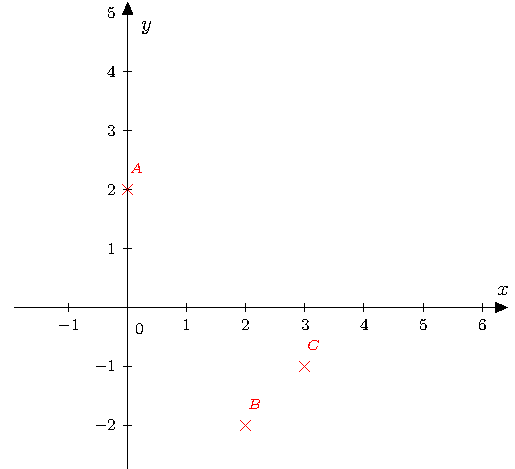
\includegraphics[width=\textwidth]{./parabelfit.pdf}
 % parabelfit.pdf: 0x0 pixel, 300dpi, 0.00x0.00 cm, bb=
 \caption{Parabel durch drei Punkte}
 \label{fig:parabelfit}
\end{figure}
 Gegeben seien die drei Punkte \(P(0|2)\), \(Q(2|-2)\) und \(R(3|-1)\). Gesucht ist die quadratische Funktion, deren Graph durch diese drei Punkte verläuft.
 
 In den Ansatz \(f(x)=ax^2+bx+c=y\) werden die Koordinaten eingesetzt:
 \begin{align*}
  \text{I} && a\cdot 0^2 + b\cdot 0 +c &= 2 \\
  \text{II} && a\cdot 2^2 + b \cdot 2 + c &= -2 \\
  \text{III} && a\cdot 3^2 + b \cdot 3 + c &= -1 
 \end{align*}
 Aus Gleichung~I folgt sofort \(c=2\). Einsetzen in die anderen beiden Gleichungen liefert:
 \begin{align*}
  \text{II'} && 4a + 2b &= -4 \\
  \text{III'} && 9a + 3b &= -3
 \end{align*}
 Auflösen von II' nach \(b\):
 \begin{align*}
  2b &= -4-4a \\
  b &= -2-2a
 \end{align*}
 Einsetzen von \(b\) in III':
 \begin{align*}
  9a+3(-2-2a) &= -3\\
  9a-6-6a &= -3 \\
  3a &= 3 \\
  a&=1\\
  \intertext{Rückeinsetzen:}
  b &= -4
 \end{align*}

 Die gesuchte Funktionsgleichung ist also:
 \begin{equation*}
  f(x) = x^2-4x+2
 \end{equation*} 

\end{bsp}




\chapter{Geometrie der 9.~Jahrgangsstufe}
\epigraph{Wo Materie ist, dort ist auch Geometrie.}{\textit{De fundamentis astrologiae certioribus}\\\textsc{Johannes Kepler}}

\section{Satzgruppe des Pythagoras}

\textsc{Pythagoras von Samos} wurde um 570~v.Chr. geboren. Nachdem er Ägypten und Babylon bereist hatte, ließ er sich um 530~v.Chr. im Süden des heutigen Italien nieder und gründete dort einen Orden. Ziel des Ordens der \emph{Pythagoreer} war vor allem eine harmonische Lebensführung. Die Pythagoreer hatten starken politischen Einfluss und waren wirtschaftlich erfolgreich. Um 510~v.Chr. wurde Pythagoras aus Kroton vertrieben. Er ging mit seinen Anhängern nach Metapont, wo er auch starb. Er hinterließ seine Frau und seine Tochter \textsc{Myia}, die selbst zu einer bedeutenden Philosophin ihrer Zeit werden sollte.

Pythagoras unterrichtete seine Anhänger in Philosophie und Mathematik. Viele seiner Kenntnisse brachte er aber von seinen Reisen aus Babylon und Ägypten mit, sodass heute nicht mehr geklärt werden kann, was wirklich von ihm selbst entdeckt worden war. Der \emph{Satz des Pythagoras} war als Rechenvorschrift vermutlich schon den Babyloniern vor 1650~v.Chr. bekannt.\footnote{Die Keilschrifttafel \emph{Plimpton~322} enthält eine Tabelle pythatoreischer Tripel.} 

Die Sätze der \emph{Satzgruppe des Pythagoras} erlauben Berechnungen der Seitenlängen und der Höhe von rechtwinkligen Dreiecken. Sie sind nur auf rechtwinklige Dreiecke anwendbar.

Die längste Seite in einem rechtwinkligen Dreieck wird als \emph{Hypotenuse}\footnote{Der Begriff \emph{Hypotenuse} stammt von den altgriechischen Begriffen \emph{hypo} für "`unten"' und \emph{teinein} für "`spannen"' oder "`sich erstrecken"'.} bezeichnet. Die beiden kurzen Seiten heißen \emph{Katheten}. Der Mittelpunkt des Umkreises eines rechtwinkligen Dreiecks ist der Mittelpunkt der Hypotenuse. Diesen Umkreis nennt man den \emph{Thaleskreis}.

\begin{figure}\begin{center}
               \begin{tikzpicture}[x=1cm,y=1cm]
\draw (0,0)  coordinate (A)  -- node[below,sloped] { Hypotenuse \(c\)} (5,0) coordinate (B) -- node[above,sloped] {Kathete \(a\)} +(143.1:4) coordinate (C) -- node[above,sloped] {Kathete \(b\)} (A);
\draw (A) node[anchor=north east] (An){\(A\)};
\draw (B) node [anchor=north west] (Bn) {\(B\)};
\draw (C) node [anchor=south] (Cn) {\(C\)};
% \draw[dashed] (2.5,0) circle (2.5cm);
\path[draw=blue, dashed,
  postaction={decorate ,decoration={text along path,
    text={\ Thaleskreis\ }, text align=center,
    text effects/.cd,  
    every character/.style={fill=white, yshift=-0.5ex}}}]
  (2.5, 2.5) arc [start angle=-270, end angle=90, radius=2.5];

\clip (A)--(B)--(C);
\draw (C) circle (0.5cm);
\fill[black] (C) ++(-80:0.25) circle (1pt);
\draw (A) circle (1cm);
\draw (B) circle (1.5cm);
\draw (A) ++(30:0.6) node{\(\alpha\)};
\draw (B) ++(165:1) node{\(\beta\)};


\end{tikzpicture}\end{center}
\caption{Benennungen im rechtwinkligen Dreieck}
\end{figure}

\subsection{Kathetensatz}

\begin{ssatz}[Kathetensatz]
 Der Flächeninhalt des Quadrats über einer Kathete entspricht dem Flächeninhalt des Rechtecks über der Hypotenuse, dessen zweite Seitenlänge der zugehörige Hypotenusenabschnitt bildet.
 
 \begin{blockwhitebox}
 \begin{equation*}  a^2 = p\cdot c \qquad b^2 = q\cdot c
 \end{equation*}
 \end{blockwhitebox}
 
 \begin{figure}\begin{center}
               \begin{tikzpicture}[x=1cm,y=1cm]
\tkzDefPoint(0,0){A}
\tkzLabelPoint[left](A){$A$}
\tkzDefPoint(5,0){B}
\tkzLabelPoint[right](B){$B$}
\tkzDrawTriangle[two angles=30 and 60](A,B) \tkzGetPoint{C}
\tkzLabelPoint[above](C){$C$}
\tkzMarkRightAngle(A,C,B)
\tkzLabelSegment[below,sloped](A,B){$c$}
\tkzLabelSegment[below,sloped,red](B,C){$a$}
\tkzLabelSegment[above,sloped](A,C){$b$}

\tkzDrawAltitude(A,B)(C) \tkzGetPoint{H}
\tkzLabelPoint[above left](H){$H$}
\tkzLabelSegment[left](H,C){$h$}
\tkzMarkRightAngle(B,H,C)

\tkzDrawSquare[red](C,B) \tkzGetPoints{D}{E}
\tkzLabelSegment[above,red,sloped](E,C){$a$}
\tkzFillPolygon[red,opacity=0.2](C,B,D,E)
% \tkzDefMidPoint(C,D) \tkzGetPoint{M}
% \tkzDrawPoint(M)
% \tkzLabelPoint[](M){$a^2$}
\tkzLabelSegment[anchor=center,red](C,D){$a^2$}

\tkzDefSquare(B,H) \tkzGetPoints{H1}{H2}
\tkzDrawArc[color=gray,towards,delta=10](B,H)(H2)

\tkzDefLine[orthogonal=through A](B,H) \tkzGetPoint{H3}
% \tkzInterLL(H1,H2)(A,H3) \tkzGetPoint{H4}
\tkzDrawPolygon[red](A,H3,H2,B)
\tkzFillPolygon[red,opacity=0.2](A,H3,H2,B)

\tkzLabelSegment[right,red](H2,B){$p$}
\tkzLabelSegment[below,red](H2,H3){$c$}

\begin{scope}[yshift=4cm, scale=0.4]
\tkzDefPoint(0,0){A2}
\tkzLabelPoint[left](A2){$A$}
\tkzDefPoint(5,0){B2}
\tkzLabelPoint[right](B2){$B$}
\tkzDrawTriangle[two angles=30 and 60](A2,B2) \tkzGetPoint{C2}
\tkzLabelPoint[above](C2){$C$}
\tkzMarkRightAngle(A2,C2,B2)
\tkzLabelSegment[below,sloped](A2,B2){$c$}
\tkzLabelSegment[above,sloped](B2,C2){$a$}
\tkzLabelSegment[below,sloped,green!50!black](A2,C2){$b$}

\tkzDrawAltitude(A2,B2)(C2) \tkzGetPoint{I}
% \tkzLabelPoint[above left](I){$H$}
% \tkzLabelSegment[left](I,C2){$h$}
\tkzMarkRightAngle(B2,I,C2)

\tkzDrawSquare[green!50!black](A2,C2) \tkzGetPoints{D2}{E2}
\tkzLabelSegment[above,green!50!black,sloped](D2,C2){$b$}
\tkzFillPolygon[green,opacity=0.2](A2,C2,D2,E2)
\tkzLabelSegment[anchor=center,green!50!black](A2,D2){$b^2$}

\tkzDefSquare(I,A2) \tkzGetPoints{I1}{I2}
\tkzDrawArc[color=gray,towards,delta=10](A2,I1)(I)

\tkzDefLine[orthogonal=through B2](I,A2) \tkzGetPoint{I3}
% \tkzInterLL(H1,H2)(A,H3) \tkzGetPoint{H4}
\tkzDrawPolygon[green!50!black](A2,I1,I3,B2)
\tkzFillPolygon[green,opacity=0.2](A2,I1,I3,B2)

 \tkzLabelSegment[left,green!50!black](I1,A2){$q$}
 \tkzLabelSegment[below,green!50!black](I1,I3){$c$}
\end{scope}
\end{tikzpicture}

\end{center}
\caption{Veranschaulichung des Kathetensatzes}
\end{figure}
\end{ssatz}

\begin{bew}
 Der Kathetensatz ergibt sich aus der Ähnlichkeit des Dreiecks \(\triangle ABC\) zum Dreieck \(\triangle CBH\). Diese Dreiecke sind ähnlich, da sie zwei Winkel gemeinsam haben: Den rechten Winkel bei \(C\) bzw. \(H\) und den Winkel \(\beta\).
 
 In diesen ähnlichen Dreiecken sind die Verhältnisse einander entsprechender Streckenlängen gleich. Also gilt:
 \begin{align*}
  \frac{p}{a} &= \frac{a}{c} && |\cdot a \cdot c \\
  pc &= a^2
 \end{align*}
 Einfaches Umformen der Gleichung der Seitenverhältnisse liefert also direkt den Kathetensatz.
\end{bew}

Der Beweis für den Kathetensatz für die Kathete \(b\) verläuft analog.

Mit Hilfe des Kathetensatzes lässt sich zu jedem Rechteck ein flächengleiches Quadrat konstruieren.

\begin{beme}[Flächengleiches Quadrat]
 Die Konstruktion eines flächengleichen Quadrats aus einem Rechteck mit gegebenen Seitenlägen \(c\) und \(p\) kann über die Anwendung des Kathetensatzes erfolgen. Es sei \(c=[AB]\). Folgende Konstruktionsschritte sind erforderlich:
 \begin{enumerate}
  \item Trage \(p\) an \(c\) ab. Das ergibt Punkt \(H\).
  \item Errichte einen Halbkreis \(k\) über \(c\).
  \item Errichte das Lot \(h\) zu \(c\) durch \(H\).
  \item Der Schnittpunkt von \(h\) mit \(k\) ergibt den Punkt \(C\). Das Quadrat über \([CB]\) hat den gleichen Flächeninhalt.
 \end{enumerate}
\end{beme}


\subsection{Satz des Pythagoras}

\begin{ssatz}[Satz des Pythagoras]
 Der Flächeninhalt des Quadrats über der Hypotenuse entspricht der Summe der Flächeninhalte der Quadrate über den Katheten.
  \begin{blockwhitebox}
 \begin{equation*}  a^2 + b^2 = c^2
 \end{equation*}
 \end{blockwhitebox}
   \begin{figure}\begin{center}
               \begin{tikzpicture}[x=1cm,y=1cm,scale=0.8]
\tkzDefPoint(0,0){A}
\tkzLabelPoint[left](A){$A$}
\tkzDefPoint(5,0){B}
\tkzLabelPoint[below right](B){$B$}
\tkzDrawTriangle[two angles=30 and 60](A,B) \tkzGetPoint{C}
\tkzLabelPoint[above](C){$C$}
\tkzMarkRightAngle(A,C,B)
\tkzLabelSegment[below,sloped](A,B){$c$}
\tkzLabelSegment[above,sloped](B,C){$a$}
\tkzLabelSegment[above,sloped](A,C){$b$}

\tkzDrawAltitude(A,B)(C) \tkzGetPoint{H}
% \tkzLabelPoint[above left](H){$H_c$}
\tkzLabelSegment[left](H,C){$h$}
\tkzMarkRightAngle(B,H,C)

\tkzDrawSquare[red](C,B) \tkzGetPoints{D}{E}
\tkzLabelSegment[above,red,sloped](E,C){$a$}
\tkzFillPolygon[red,opacity=0.2](C,B,D,E)
\tkzLabelSegment[anchor=center,red](C,D){$a^2$}

\tkzDrawSquare[green!50!black](A,C) \tkzGetPoints{D2}{E2}
\tkzLabelSegment[above,green!50!black,sloped](D2,C){$b$}
\tkzFillPolygon[green,opacity=0.2](A,C,D2,E2)
\tkzLabelSegment[anchor=center,green!50!black](A,D2){$b^2$}

\tkzDrawSquare[blue](B,A) \tkzGetPoints{F}{G}
\tkzLabelSegment[left,blue](A,F){$c$}
\tkzFillPolygon[blue,opacity=0.2](A,F,G,B)
\tkzLabelSegment[anchor=center,blue](A,G){$c^2$}

\end{tikzpicture}\end{center}
\caption{Veranschaulichung des Satz des Pythagoras}
\end{figure}
\end{ssatz}

Für den Satz des Pythagoras sind heute über 400 verschiedene Beweise bekannt. Eine kleine Auswahl wird hier präsentiert.

\begin{bew}[Arithmetischer Beweis]

Über der Hypotenuse des rechtwinkligen Dreiecks \(\triangle ABC\) wird das Quadrat errichtet. An die anderen drei Seiten dieses Quadrats wird wieder das Ausgangsdreieck nach innen angefügt.
\begin{figure}\begin{center}
               \begin{tikzpicture}[x=1cm,y=1cm,scale=0.8]
\tkzDefPoint(0,0){A}
\tkzLabelPoint[below left](A){$A$}
\tkzDefPoint(5,0){B}
\tkzLabelPoint[below right](B){$B$}
\tkzDrawTriangle[two angles=30 and 60](A,B) \tkzGetPoint{C}
\tkzLabelPoint[above right](C){$C$}
\tkzMarkRightAngle(A,C,B)
\tkzLabelSegment[below,sloped](A,B){$c$}
\tkzLabelSegment[below,sloped](B,C){$a$}
\tkzLabelSegment[below,sloped](A,C){$b$}

\tkzDrawSquare[](A,B)\tkzGetPoints{A2}{B2}
\tkzLabelPoint[above right](A2){$A'$}
\tkzLabelPoint[above left](B2){$B'$}
\tkzDrawTriangle[two angles=30 and 60](B,A2) \tkzGetPoint{C2}
\tkzLabelPoint[above left](C2){$D$}
\tkzMarkRightAngle(B,C2,A2)
\tkzDrawTriangle[two angles=30 and 60](A2,B2) \tkzGetPoint{C3}
\tkzLabelPoint[below left](C3){$E$}
\tkzMarkRightAngle(A2,C3,B2)
\tkzDrawTriangle[two angles=30 and 60](B2,A) \tkzGetPoint{C4}
\tkzLabelPoint[below right](C4){$F$}
\tkzMarkRightAngle(B2,C4,A)
\tkzFillPolygon[red,opacity=0.2](C,C2,C3,C4)

\tkzDefMidPoint(C,C3)\tkzGetPoint{M}
\tkzLabelPoint[anchor=center,red](M){$(b-a)^2$}

 \end{tikzpicture}\end{center}
\caption{Figur zum Arithmetischen Beweis des Satz des Pythagoras}
\end{figure}
Daraus ergibt sich das neue Quadrat \(\square CDEF\) mit dem Flächeninhalt:
\begin{align*}
 A_{\square CDEF} &= (b-a)^2 = b^2 -2ab +a^2
\end{align*}
Den Flächeninhalt von \(\square CDEF\) kann man aber auch auf eine zweite Weise bestimmen. Diesen Flächeninhalt erhält man, wenn man vom Hypotenusenquadrat \(\square ABA'B'\) viermal die Fläche des Ausgangsdreicks \(\triangle ABC\) subtrahiert.
\begin{align*}
 A_{\square CDEF} &= A_{\square ABA'B'} - 4\cdot A_{\triangle ABC} \\
 &= c^2 - 4\cdot \frac{1}{2}ab \\
 \intertext{Einsetzen des ersten Terms:}
 (b-a)^2 &= c^2 - 2ab \\
 b^2 -2ab + a^2 &= c^2 - 2ab && | +2ab \\
 b^2 + a^2 &= c^2
\end{align*}

\end{bew}

\begin{bew}[Chinesischer Ergänzungsbeweis]
  Die\-se Vi\-su\-a\-li\-sie\-rung -- kein echter Beweis im logischen Sinn -- findet man im Kommentar zum ersten Buch von Euklids \emph{Elementen} von \textsc{Proklos}, in hinduistischen Schriften und im chinesischen \emph{Zhoubi suanjing} (ca.~100~v.Chr.). Dieser Nachweis ergänzt zum Ausgangsdreieck kongruente Dreiecke außen an das Hypotenusenquadrat. Das sich ergebende Quadrat \(\square CDEF\) lässt sich dann durch eine Umordnung der vier kongruenten Dreiecke innerhalb seiner Fläche auch in zwei Rechtecke mit den Seitenlängen \(a\) und \(b\), sowie in zwei Quadrate mit den Flächeninhalten \(a^2\) und \(b^2\) zerlegen.\footnote{Auch bekannt als \emph{Altindischer Ergänzungsbeweis}}
 \begin{figure}\begin{center}
               \begin{tikzpicture}[x=1cm,y=1cm,scale=0.8]
\begin{scope}[xshift=-2.5cm, scale=0.4]                              
\tkzDefPoint(0,0){A}
% \tkzLabelPoint[below left](A){$A$}
\tkzDefPoint(5,0){B}
% \tkzLabelPoint[below right](B){$B$}
\tkzDrawTriangle[two angles=30 and 60](A,B) \tkzGetPoint{C}
\tkzLabelPoint[above](C){$C$}
\tkzMarkRightAngle(A,C,B)
% \tkzLabelSegment[above,sloped](A,B){$c$}
\tkzLabelSegment[above,sloped](B,C){$a$}
\tkzLabelSegment[above,sloped](A,C){$b$}

\tkzDrawSquare[](B,A)\tkzGetPoints{A2}{B2}
% \tkzLabelPoint[above right](A2){$A'$}
% \tkzLabelPoint[above left](B2){$B'$}
\tkzDrawTriangle[two angles=30 and 60](A2,A) \tkzGetPoint{C2}
\tkzLabelPoint[left](C2){$D$}
\tkzMarkRightAngle(A2,C2,A)
\tkzDrawTriangle[two angles=30 and 60](B2,A2) \tkzGetPoint{C3}
\tkzLabelPoint[below](C3){$E$}
\tkzMarkRightAngle(B2,C3,A2)
\tkzDrawTriangle[two angles=30 and 60](B,B2) \tkzGetPoint{C4}
\tkzLabelPoint[right](C4){$F$}
\tkzMarkRightAngle(B,C4,B2)
\tkzFillPolygon[blue,opacity=0.2](A,A2,B2,B)

\tkzDefMidPoint(A,B2)\tkzGetPoint{M}
\tkzLabelPoint[anchor=center,blue](M){$c^2$}
\end{scope}
\begin{scope}[xshift=2.5cm, scale=0.4]                              
\tkzDefPoint(0,0){A}
% \tkzLabelPoint[below left](A){$A$}
\tkzDefPoint(5,0){B}
% \tkzLabelPoint[below right](B){$B$}
\tkzDrawTriangle[two angles=30 and 60](A,B) \tkzGetPoint{C}
\tkzLabelPoint[above](C){$C$}
\tkzMarkRightAngle(A,C,B)
% \tkzLabelSegment[below,sloped](A,B){$c$}
\tkzLabelSegment[above,sloped](B,C){$a$}
\tkzLabelSegment[above,sloped](A,C){$b$}
\tkzDefTriangle[two angles=30 and 60](B,A) \tkzGetPoint{D}
\tkzMarkRightAngle(B,D,A)
\tkzDrawSquare[](D,A)\tkzGetPoints{E}{F}
\tkzLabelPoint[left](E){$D$}
\tkzDrawSquare[](B,D)\tkzGetPoints{G}{H}
\tkzDrawTriangle[two angles=60 and 30](G,F) \tkzGetPoint{I}
\tkzMarkRightAngle(F,D,G)
\tkzMarkRightAngle(G,I,F)
\tkzLabelPoint[below](I){$E$}
\tkzLabelPoint[right](H){$F$}
\tkzFillPolygon[red,opacity=0.2](A,E,F,D)
\tkzFillPolygon[green,opacity=0.2](B,D,G,H)
\tkzDefMidPoint(A,F)\tkzGetPoint{M}
\tkzLabelPoint[anchor=center,red](M){$a^2$}
\tkzDefMidPoint(B,G)\tkzGetPoint{N}
\tkzLabelPoint[anchor=center,green!50!black](N){$b^2$}
\end{scope}
 \end{tikzpicture}\end{center}
 \caption{Figur zum Chinesischen Ergänzungsbeweis des Satz des Pythagoras}
\end{figure}
Stellt man den Term für die Fläche von \(\square CDEF\) auf, erhält man:
 \begin{align*}
  A_{\square CDEF} &= c^2 + 4 \cdot \frac{1}{2}ab \\
  \intertext{aber auch:}
  A_{\square CDEF} &= a^2 + b^2 + 2ab \\
  \intertext{Gleichsetzen liefert:}
  c^2 + 2ab &= a^2 + b^2 + 2ab \\
  c^2 &= a^2 + b^2
 \end{align*}
\end{bew}


\begin{bew}[Beweis nach \textsc{Euklid}]

Der nächste Beweis ist im ersten Buch der Elemente des \textsc{Euklid} zu finden. Der Beweis fußt auf einer Abfolge von drei flächenerhaltenden Transformationen.\footnote{flächenerhaltende Transformationen sind: Verschiebung, Drehung, Spiegelung und Scherung.}

 \begin{figure}\begin{center}
               \begin{tikzpicture}[x=1cm,y=1cm,scale=0.8]
               \small
\begin{scope}[xshift=-2.5cm, yshift=2.5cm, scale=0.4]                              
\tkzDefPoint(0,0){A}
\tkzLabelPoint[below left](A){$A$}
\tkzDefPoint(5,0){B}
\tkzLabelPoint[below right](B){$B$}
\tkzDrawTriangle[two angles=30 and 60](A,B) \tkzGetPoint{C}
\tkzLabelPoint[above](C){$C$}
\tkzMarkRightAngle(A,C,B)
% \tkzLabelSegment[below,sloped](A,B){$c$}
% \tkzLabelSegment[below,sloped](B,C){$a$}
% \tkzLabelSegment[below,sloped](A,C){$b$}

\tkzDrawSquare[](A,C)\tkzGetPoints{D}{E}
\tkzLabelPoint[above ](D){$D$}
\tkzLabelPoint[above left](E){$E$}
\tkzDefMidPoint(A,D)\tkzGetPoint{M}
\tkzLabelPoint[anchor=center,green!50!black](M){$b^2$}
\tkzFillPolygon[green,opacity=0.2](A,C,D,E)

\tkzDrawSquare[](C,B)\tkzGetPoints{F}{G}
\tkzLabelPoint[above ](G){$G$}
\tkzLabelPoint[above right](F){$F$}
\tkzDefMidPoint(B,G)\tkzGetPoint{N}
\tkzLabelPoint[anchor=center,red](N){$a^2$}
\tkzFillPolygon[red,opacity=0.2](C,B,F,G)
\tkzInterLL(E,D)(G,F) \tkzGetPoint{P}
\tkzDrawVector[gray](D,P)
\tkzDrawVector[gray](G,P)
\end{scope}
\begin{scope}[xshift=2.5cm,yshift=2.5cm, scale=0.4]                              
\tkzDefPoint(0,0){A2}
% \tkzLabelPoint[below left](A){$A$}
\tkzDefPoint(5,0){B2}
% \tkzLabelPoint[below right](B){$B$}
\tkzDrawTriangle[two angles=30 and 60](A2,B2) \tkzGetPoint{C2}
% \tkzLabelPoint[below](C2){$C$}
\tkzMarkRightAngle(A2,C2,B2)
\tkzDrawAltitude[dashed](A2,B2)(C2) \tkzGetPoint{H2}
\tkzDrawSquare[](A2,C2)\tkzGetPoints{D2}{E2}
\tkzDrawSquare[](C2,B2)\tkzGetPoints{F2}{G2}
\tkzInterLL(E2,D2)(G2,F2) \tkzGetPoint{P2}
\tkzLabelPoint[above](P2){$P$}
\tkzDefLine[orthogonal=through A2](A2,B2) \tkzGetPoint{Y2}
\tkzInterLL(E2,D2)(A2,Y2) \tkzGetPoint{R2}
\tkzFillPolygon[green,opacity=0.2](A2,C2,P2,R2)

\tkzDefLine[orthogonal=through B2](A2,B2) \tkzGetPoint{Z2}
\tkzInterLL(F2,G2)(B2,Z2) \tkzGetPoint{S2}
\tkzFillPolygon[red,opacity=0.2](C2,B2,Z2,P2)

\tkzDrawSegment[dashed](C2,P2)
\tkzDrawSegment[dashed](D2,P2)
\tkzDrawSegment[dashed](G2,P2)
\tkzDrawSegment[dotted](A2,Y2)
\tkzDrawSegment[dotted](B2,Z2)
\end{scope}
\begin{scope}[xshift=+2.5cm,yshift=-2cm, scale=0.4]                              
\tkzDefPoint(0,0){A3}
% \tkzLabelPoint[below left](A){$A$}
\tkzDefPoint(5,0){B3}
% \tkzLabelPoint[below right](B){$B$}
\tkzDrawTriangle[two angles=30 and 60](A3,B3) \tkzGetPoint{C3}
% \tkzLabelPoint[below](C2){$C$}
\tkzMarkRightAngle(A3,C3,B3)
\tkzDrawAltitude[dashed](A3,B3)(C3) \tkzGetPoint{H3}
\tkzLabelPoint[below](H3){$H$}
\tkzDrawSquare[](A3,C3)\tkzGetPoints{D3}{E3}
\tkzDrawSquare[](C3,B3)\tkzGetPoints{F3}{G3}
\tkzInterLL(E3,D3)(G3,F3) \tkzGetPoint{P3}
\tkzDefLine[orthogonal=through A3](A3,B3) \tkzGetPoint{Y3}
\tkzInterLL(E3,D3)(A3,Y3) \tkzGetPoint{R3}

\tkzDefLine[orthogonal=through B3](A3,B3) \tkzGetPoint{Z3}
\tkzInterLL(F3,G3)(B3,Z3) \tkzGetPoint{S3}
\tkzInterLL(C3,H3)(Y3,Z3) \tkzGetPoint{T3}
\tkzFillPolygon[green,opacity=0.2](A3,H3,T3,Y3)
\tkzFillPolygon[red,opacity=0.2](H3,B3,Z3,T3)

\tkzDrawSegment[dashed](C3,P3)
\tkzDrawSegment[dashed](D3,P3)
\tkzDrawSegment[dashed](G3,P3)
\tkzDrawSquare[dotted](A3,B3)
\end{scope}
\begin{scope}[xshift=-2.5cm,yshift=-2cm, scale=0.4]                              
\tkzDefPoint(0,0){A4}
% \tkzLabelPoint[below left](A){$A$}
\tkzDefPoint(5,0){B4}
% \tkzLabelPoint[below right](B){$B$}
\tkzDrawTriangle[two angles=30 and 60](A4,B4) \tkzGetPoint{C4}
% \tkzLabelPoint[below](C2){$C$}
\tkzMarkRightAngle(A4,C4,B4)
\tkzDrawAltitude[dashed](A4,B4)(C4) \tkzGetPoint{H4}
\tkzDrawSquare[](A4,C4)\tkzGetPoints{D4}{E4}
\tkzDrawSquare[](C4,B4)\tkzGetPoints{F4}{G4}
\tkzInterLL(E4,D4)(G4,F4) \tkzGetPoint{P4}
\tkzDefLine[orthogonal=through A4](A4,B4) \tkzGetPoint{Y4}
\tkzInterLL(E4,D4)(A4,Y4) \tkzGetPoint{R4}

\tkzDefLine[orthogonal=through B4](A4,B4) \tkzGetPoint{Z4}
\tkzInterLL(F4,G4)(B4,Z4) \tkzGetPoint{S4}
\tkzInterLL(C4,H4)(Y4,Z4) \tkzGetPoint{T4}
\tkzDrawSquare[blue](B4,A4)\tkzGetPoints{I4}{J4}
\tkzInterLL(C4,H4)(I4,J4) \tkzGetPoint{Q4}

\tkzFillPolygon[green,opacity=0.2](A4,I4,Q4,H4)
\tkzFillPolygon[red,opacity=0.2](H4,Q4,J4,B4)

\tkzDrawSegment[dashed](C4,P4)
\tkzDrawSegment[dashed](D4,P4)
\tkzDrawSegment[dashed](G4,P4)
\tkzDrawSquare[dotted](A4,B4)
\end{scope}
\tkzDrawVector[gray](P,P2)
\tkzLabelSegment[sloped,above,gray](P,P2){Scherung}
\tkzDrawVector[gray](C2,T3)
\tkzLabelSegment[right,gray](C2,T3){Scherung}
\tkzDrawVector[gray](T3,H4)
\tkzLabelSegment[sloped,above,fill=white,opacity=0.5](T3,H4){Verschiebung}

\end{tikzpicture}\end{center}
 \caption{Beweis nach \textsc{Euklid}}
\end{figure}

Ausgangspunkt ist das rechtwinklige Dreieck über dessen Katheten die Quadrate errichtet werden. Im ersten Schritt werden die Quadrate einer Scherung entlang von Parallelen zu den Katheten unterzogen, sodass die Punkte \(D\) und \(G\) auf dem Punkt \(P\) zu liegen kommen. \(P\) befindet sich in der Verlängerung der Höhe von Dreieck \(\triangle ABC\). So erhält man zwei Parallelogramme, die eine Seite gemeinsam haben. Die Parallelogramme haben die Flächeninhalte \(a^2\) und \(b^2\).

Der zweite Schritt besteht darin, dass die Parallelogramme ein zweites Mal einer Scherung unterzogen werden. Dabei kommt der Punkt \(C\) auf dem Höhenfußpunkt \(H\) zu liegen. Man erhält zwei Rechtecke, die gemeinsam ein Quadrat ergeben, dessen Seitenlänge der Hypotenuse \(c\) entspricht.

Um zuletzt noch zu zeigen, dass das Quadrat, das durch die beiden Scherungen entstanden ist, das Hypotenusenquadrat ist, kann man es noch nach unten verschieben.

Da weder Scherung noch Verschiebung einen Flächeninhalt ändern, folgt daraus, dass \(a^2+b^2 = c^2\).

\end{bew}

\begin{satz}[Umkehrung des Satz des Pythagoras]
 Ergibt die Summe der Quadrate zweier Seitenlängen im Quadrat das Quadrat der dritten Seitenlänge, so ist das Dreieck ein rechtwinkliges. Kurz:
 \begin{align*}
  a^2+b^2&=c^2&&\Rightarrow & \triangle ABC & \quad\text{ ist rechtwinklig.} 
 \end{align*}
\end{satz}

\begin{defi}[Pythagoreisches Tripel]
 Unter einem \emph{Pythagoreischen Tripel} versteht man eine Menge von drei ganzen Zahlen, die den Satz des Pythagoras erfüllen. Das bekannteste solche Tripel ist \((3,4,5)\), denn:
 \begin{equation*}
  3^2+4^2 = 9 +16 =25 =5^2
 \end{equation*}
 Andere Pythagoreische Tripel sind: \((5;12;13)\), \((8;15;17)\) oder \((20;21;29)\).
\end{defi}


\begin{beme}
 Auf der Umkehrung des Satz des Pythagoras beruht auch die oft von Handwerkern benutzte 3-4-5-Regel: Verhalten sich die in einem Dreieck die Seitenlägen wie 3 zu 4 zu 5, dann handelt es sich um ein rechtwinkliges.
\end{beme}


\subsection{Höhensatz}

\begin{ssatz}[Höhensatz]
   Der Flächeninhalt des Quadrats über der Höhe eines rechtwinkligen Dreiecks entspricht dem Flächeninhalt des Rechtecks der Hypotenusenabschnitte.
    \begin{blockwhitebox}
 \begin{equation*} h^2 = p\cdot q
 \end{equation*}
 \end{blockwhitebox}
 \begin{figure}\begin{center}
               \begin{tikzpicture}[x=1cm,y=1cm]\tkzInit[xmin=0, ymin=-1.5,xmax=6.5, ymax=2.5] \tkzClip[space=.5]
\tkzDefPoint(0,0){A}
\tkzLabelPoint[left](A){$A$}
\tkzDefPoint(5,0){B}
\tkzLabelPoint[below right](B){$B$}
\tkzDrawTriangle[two angles=30 and 60](A,B) \tkzGetPoint{C}
\tkzLabelPoint[above](C){$C$}
\tkzMarkRightAngle(A,C,B)
\tkzLabelSegment[below,sloped](A,B){$c$}
\tkzLabelSegment[above,sloped](B,C){$a$}
\tkzLabelSegment[above,sloped](A,C){$b$}

\tkzDrawAltitude(A,B)(C) \tkzGetPoint{H}
% \tkzLabelPoint[above left](H){$H_c$}
\tkzLabelSegment[left,red](H,C){$h$}
\tkzMarkRightAngle(B,H,C)

\tkzDrawSquare[red](C,H) \tkzGetPoints{D}{E}
\tkzLabelSegment[above,red](E,C){$h$}
\tkzFillPolygon[red,opacity=0.2](C,H,D,E)


\tkzDefSquare(B,H) \tkzGetPoints{H1}{H2}
\tkzDrawArc[color=gray,towards,delta=10](H,H1)(B)

\tkzDefLine[orthogonal=through A](A,B) \tkzGetPoint{H3}
\tkzInterLL(H1,H2)(A,H3) \tkzGetPoint{H4}
\tkzDrawPolygon[red](H,H1,H4,A)
\tkzFillPolygon[red,opacity=0.2](H,H1,H4,A)

\tkzLabelSegment[below,red](H4,H1){$q$}
\tkzLabelSegment[right,red](H,H1){$p$}

\end{tikzpicture}\end{center}
\caption{Veranschaulichung des Höhensatzes}
\end{figure}
\end{ssatz}

\begin{bew}[Ergänzungsbeweis]
 Der Höhensatz lässt sich dadurch zeigen, dass man die Figur zu einem Rechteck ergänzt. (s. Abb.~\ref{abb:bewHSatz}) Betrachte dann das Dreieck \(\triangle PQR\). Sein Flächeninhalt lässt sich auf zwei Arten berechnen. Einerseits entspricht der Flächeninhalt der Hälfte des Rechtecks mit den Seitenlängen \(q+h\) und \(p+h\). Andererseits setzt sich das Dreiecks aus dem Rechteck mit den Seitenlängen \(p\) und \(q\), sowie den Hälften der Rechtecke mit den Seitenlängen \(q\) und \(h\) bzw. \(p\) und \(h\) zusammen.
 \begin{figure}\begin{center}
               \begin{tikzpicture}[x=1cm,y=1cm]
\tkzInit[xmin=0, ymin=-3,xmax=5, ymax=2.5] \tkzClip[space=.5]
\tkzDefPoint(0,0){A}
\tkzLabelPoint[left](A){$A$}
\tkzDefPoint(5,0){B}
\tkzLabelPoint[below right](B){$B$}
\tkzDrawTriangle[two angles=50 and 40](A,B)\tkzGetPoint{C}
\tkzLabelPoint[above](C){$C$}
\tkzMarkRightAngle(A,C,B)
% \tkzLabelSegment[below,sloped](A,B){$c$}
% \tkzLabelSegment[above,sloped](B,C){$a$}
% \tkzLabelSegment[above,sloped](A,C){$b$}

\tkzDrawAltitude(A,B)(C) \tkzGetPoint{H}
% \tkzLabelPoint[above left](H){$H_c$}
% \tkzLabelSegment[left,red](H,C){$h$}
\tkzMarkRightAngle(B,H,C)

\tkzDrawSquare[red](C,H) \tkzGetPoints{D}{E}
\tkzLabelSegment[above,red](E,C){$h$}
\tkzLabelSegment[right,red](D,E){$h$}
\tkzFillPolygon[red,opacity=0.2](C,H,D,E)

\tkzDefSquare(B,H) \tkzGetPoints{H1}{H2}
\tkzDrawArc[color=gray,towards,delta=10](H,H1)(B)

\tkzDefLine[orthogonal=through A](A,B) \tkzGetPoint{H3}
\tkzInterLL(H1,H2)(A,H3) \tkzGetPoint{H4}
% \tkzLabelPoint(H4){$H_4$}
% \tkzLabelPoint(H1){$H_1$}
% \tkzLabelPoint(D){$D$}
% \tkzLabelPoint(E){$E$}
\tkzDrawPolygon[red](H,H1,H4,A)
\tkzFillPolygon[red,opacity=0.2](H,H1,H4,A)

\tkzLabelSegment[below,red](H4,H1){$q$}
\tkzLabelSegment[left,red](A,H4){$p$}

\tkzInterLL(H2,H1)(E,D) \tkzGetPoint{G}
% \tkzLabelPoint(G){$G$}
\tkzDrawPolygon[green](D,H,H1,G)
\tkzFillPolygon[green,opacity=0.2](D,H,H1,G)
\tkzInterLL(H4,A)(E,C) \tkzGetPoint{P}
\tkzDrawPolygon[blue](A,H,C,P)
\tkzFillPolygon[blue,opacity=0.2](A,H,C,P)
\tkzDrawSegment[dotted](P,G)

\tkzLabelSegment[below,green!50!black](H1,G){$h$}
\tkzLabelSegment[right,green!50!black](D,G){$p$}
\tkzLabelSegment[above,blue](P,C){$q$}
\tkzLabelSegment[left,blue](A,P){$h$}
\tkzLabelPoint[above left](P){$P$}
\tkzLabelPoint[below left](H4){$Q$}
\tkzLabelPoint[below right](G){$R$}
\end{tikzpicture}\end{center}
\caption{Beweisfigur zum Höhensatz}
\label{abb:bewHSatz}
\end{figure}
\begin{align*}
 A_{\triangle PQR} = \frac{1}{2} (p+h)(q+h) &= pq + \frac{1}{2}qh + \frac{1}{2}ph \\
                     \frac{1}{2} \left(pq +ph +qh + h^2\right) &= pq + \frac{1}{2}qh + \frac{1}{2}ph \\
                     \frac{1}{2} pq + \frac{1}{2} ph + \frac{1}{2} qh + \frac{1}{2} h^2 &= pq + \frac{1}{2}qh + \frac{1}{2}ph \\
                     \frac{1}{2} h^2 &= \frac{1}{2} pq \\
                     h^2 &= pq
\end{align*}

\end{bew}

\subsection{Dreiecksberechnungen}

\begin{folg}[Berechnung der Hypotenuse]
 Aus dem Satz des Pythagoras folgt: In einem rechtwinkligen Dreieck \(\triangle ABC\) gilt für die Länge der Hypotenuse \(c\):
 \begin{align*}
  c^2 &= a^2 + b^2 &&|\sqrt{\ldots}\\
  c &= \sqrt{a^2 + b^2}
 \end{align*}
 Die Längen der Katheten legen also die Länge der Hypotenuse fest.
\end{folg}

\begin{folg}[Berechnung der Höhe]
 Die Höhe eines rechtinkligen Dreiecks kann über verschiedene Wege bestimmt werden.
 
 Sind die Hypotenusenabschnitte gegeben, so lässt sich direkt der Höhensatz anwenden.
 \begin{align*}
  h^2 &= pq & &\Rightarrow & h &=\sqrt{pq}
 \end{align*}
 
 Ist eine Kathete und der zugehörige Hypotenusenabschnitt gegeben, so gilt nach dem Satz des Pythagoras für das Teildreieck \(\triangle ACH\) oder \(\triangle BHC\):
 \begin{align*}
  h^2 + p^2 &= a^2 & &\Rightarrow& h &=\sqrt{a^2-p^2} \\
  \intertext{analog:}
  h^2 + q^2 &= b^2 & &\Rightarrow& h &=\sqrt{b^2-q^2}
 \end{align*}
\end{folg}

\begin{folg}[Berechnung der Kathetenlänge]
 Die Länge einer der Katheten kann auch über mehrere Wege, abhängig von den gegebenen Größen erfolgen:
 
 Ist die Länge der Hypotenuse \(c\) und die Länge einer Kathete \(b\) bekannt, so kann der Satz des Pythagoras angewendet werden.
 \begin{align*}
  a^2 +b^2 &= c^2 & &\Rightarrow & a &=\sqrt{c^2-b^2}
 \end{align*}
 
 Ist ein Hypotenusenabschnitt, z.B. \(p\), und die Länge der Hypotenuse \(c\) bekannt, so kann die Länge der Katheten über den Kathetensatz berechnet werden.
 \begin{align*}
  a^2 &= pc &&\Rightarrow & a&=\sqrt{pc}\\
  b^2 &= qc = (c-p)c &&\Rightarrow & b&=\sqrt{(c-p)c}
 \end{align*}
 
 Ist die Höhe \(h\) und der passende Hyptenusenabschnitt, z.B. \(p\), bekannt, so kann die Länge der Katheten auch über den Satz des Pythagoras bestimmt werden.
 \begin{align*}
  a^2 &= h^2 + p^2 && \Rightarrow & a &= \sqrt{h^2+p^2}
 \end{align*}

\end{folg}

\begin{folg}[Gleichschenkliges Dreieck]
 An einem gleichschenkligen Dreieck ist keiner der Sätze aus der Satzgruppe des Pythagoras direkt anwendbar. Doch die Höhe auf die Basis des gleichschenkligen Dreiecks teil das Dreieck in zwei rechtwinklige Dreiecke. In diesen Teildreiecken sind Satz des Pythagoras, Katheten- und Höhensatz anwendbar.
 \begin{figure}
  \begin{center}
   \begin{tikzpicture}[x=1cm,y=1cm,scale=0.6]
 \tkzInit[xmin=-0.5, ymin=-0.5,xmax=3.5, ymax=5]
   \tkzClip[space=.3]
\tkzDefPoint(0,0){A} \tkzDefPoint(3,0){B}
\tkzDefTriangle[euclide](A,B)\tkzGetPoint{C}
\tkzDrawPolygon(A,B,C)
\tkzDrawPoints(A,B,C)
\tkzLabelPoint[left](A){$A$}
\tkzLabelPoint[right](B){$B$}
\tkzLabelPoint[above](C){$C$}
\tkzLabelSegment[below](A,B){$c$}
\tkzLabelSegment[above,sloped](A,C){$a$}
\tkzLabelSegment[above,sloped](B,C){$a$}
\tkzSetUpLine[color=red]
\tkzDrawBisector(A,C,B) \tkzGetPoint{H}
\tkzMarkRightAngle(B,H,C)
\tkzLabelPoint[red,above right](H){$H$}
\tkzLabelSegment[red,left,near end](C,H){$h$}
   \end{tikzpicture}
  \end{center}
  \caption{Gleichschenkliges Dreieck}
 \end{figure}
 So lässt sich die Höhe des gleichschenkligen Dreiecks aus den Seitenlängen berechnen. Betrachte das Dreieck \(\triangle HBC\). An diesem Dreieck gilt der Satz des Pythagoras:
 \begin{align*}
  \left(\frac{c}{2}\right)^2 + h^2 &= a^2 &&| -\left(\frac{c}{2}\right)^2 \\
  h^2 &= a^2-\frac{c^2}{4} && | \sqrt{\ldots} \\
  h &= \sqrt{a^2-\frac{c^2}{4}}
 \end{align*}
 
 Ist die Höhe des Dreiecks und die Basislänge \(c\) bekannt, so kann mit der gleichen Beziehung die Länge der beiden Schenkel berechnet werden:
 \begin{align*}
  a^2 &= \left(\frac{c}{2}\right)^2 + h^2 &&|\sqrt{\ldots}\\
  a &= \sqrt{\frac{c^2}{4}+h^2}
 \end{align*}
\end{folg}

\begin{folg}[Höhe im gleichseitigen Dreieck]
 Der Satz des Pythagoras verbindet im gleichseitigen Dreieck die Höhe des Dreiecks mit der Seitenlänge. Die Höhe teilt das Dreieck in zwei rechtwinklige Dreiecke.
 
  \begin{figure}
  \begin{center}
   \begin{tikzpicture}[x=1cm,y=1cm,scale=0.75]
 \tkzInit[xmin=-0.5, ymin=-0.2,xmax=3.5, ymax=3.5]
   \tkzClip[space=.3]
\tkzDefPoint(0,0){A} \tkzDefPoint(3,0){B}
\tkzDefTriangle[equilateral](A,B)\tkzGetPoint{C}
\tkzDrawPolygon(A,B,C)
\tkzDrawPoints(A,B,C)
\tkzLabelPoint[left](A){$A$}
\tkzLabelPoint[right](B){$B$}
\tkzLabelPoint[above](C){$C$}
\tkzLabelSegment[below](A,B){$a$}
\tkzLabelSegment[above,sloped](A,C){$a$}
\tkzLabelSegment[above,sloped](B,C){$a$}
\tkzSetUpLine[color=red]
\tkzDrawBisector(A,C,B) \tkzGetPoint{H}
\tkzMarkRightAngle(B,H,C)
\tkzLabelPoint[red,above right](H){$H$}
\tkzLabelSegment[red,left](C,H){$h$}
   \end{tikzpicture}
  \end{center}
  \caption{Gleichseitiges Dreieck}
 \end{figure}
 
 Betrachte das Dreieck \(\triangle HBC\). Der Satz des Pythagoras für dieses Dreieck lautet:
 \begin{align*}
  h^2 + \left(\frac{a}{2}\right)^2 &= a^2 && |- \left(\frac{a}{2}\right)^2 \\
  h^2 &= a^2 - \frac{a^2}{4} \\
  h^2 &= \frac{3}{4} a^2 &&| \sqrt{\ldots} \\
  h &= \sqrt{\frac{3}{4} a^2} = \frac{\sqrt{3}}{2}a
 \end{align*}
 
 Somit kann man auch den Flächeninhalt des gleichseitigen Dreiecks nur in Abhängigkeit der Seitenlänge ausdrücken.
 \begin{align*}
  A_{\triangle ABC} = \frac{1}{2} \cdot a\cdot h &= \frac{1}{2} \cdot a \cdot \frac{\sqrt{3}}{2}a \\
  &= \frac{\sqrt{3}}{4}a^2
 \end{align*}

\end{folg}


\subsection{Grundkonstruktionen}


\begin{regel}[Quadrat zu Rechteck]
Diese Grundkonstruktion erfüllt die Aufgabe ein Quadrat gegebener Fläche in ein \emph{flächengleiches} Rechteck umzuwandeln.
  \begin{figure}
  \begin{center}
   \begin{tikzpicture}[x=1cm,y=1cm,scale=0.5]
%  \tkzInit[xmin=-0.5, ymin=-0.2,xmax=3.5, ymax=3.5]
%    \tkzClip[space=.3]
\tkzDefPoint(0,0){A} \tkzDefPoint(3,0){B}
\tkzDrawSquare[red](A,B)\tkzGetPoints{C}{D}
\tkzDefPoint(3,4){E}
\tkzFillPolygon[red,opacity=0.2](A,B,C,D)
\tkzDrawPoints(A,B,C,D)
\tkzLabelPoint[left](A){$A$}
\tkzLabelPoint[right](B){$B$}
\tkzLabelPoint[below,right](C){$C$}
\tkzLabelPoint[left](D){$D$}
\tkzLabelSegment[below](A,B){$h$}
\tkzLabelSegment[above,sloped](A,D){$h$}
\tkzDrawCircle[dashed,color=gray](C,E)
\tkzInterLC(C,D)(C,E) \tkzGetPoints{F}{G}
\tkzDrawSegment(C,E)
\tkzLabelSegment[left](C,E){$p$}

\tkzDrawPoint(G)
\tkzDrawSegment(G,B)
\tkzDefLine[orthogonal=through B](B,G) \tkzGetPoint{H}
\tkzMarkRightAngle(H,B,G)
\tkzInterLL(D,C)(B,H) \tkzGetPoint{I}
\tkzDrawLine[add=.5 and 3.2](H,B)
\tkzDrawLine[add=.5 and 3.2](D,C)
\tkzDrawPoint(I)
\tkzDrawPoint(E)

\tkzDefLine[orthogonal=through I](D,C) \tkzGetPoint{J}
\tkzDefLine[orthogonal=through E](B,C) \tkzGetPoint{K}
\tkzInterLL(E,K)(I,J) \tkzGetPoint{L}
\tkzDrawPoint(L)
\tkzDrawPolygon[red](C,I,L,E)
\tkzFillPolygon[red,opacity=0.2](C,I,L,E)

\end{tikzpicture}
  \end{center}
  \caption{Flächenerhaltende Umformung eines Quadrats in ein Rechteck}
 \end{figure}

\end{regel}

\begin{regel}[Flächengleiches Rechteck zu Quadrat]
 
\end{regel}

\begin{regel}[Konstruktion einer Quadratwurzel]
 
\end{regel}

\begin{regel}[Zerlegung eines Quadrats]

\end{regel}

\begin{regel}[Quadratur eines Dreiecks]
 
\end{regel}

\begin{regel}[Konstruktion von Tangenten]
 
\end{regel}

\begin{regel}[Gemeinsame Tangenten]
 
\end{regel}


\subsection{Abstand von Punkten}

\begin{folg}[Abstand in der Ebene]
Der Abstand zweier Punkte in einer Ebene kann anhand ihrer Koordinaten berechnet werden. Betrachte die Punkte \(A(x_A\mid y_A)\) und \(B(x_B\mid y_B)\). Dann gilt für deren Abstand \(d=d(A;B)\):
\begin{align*}
 d^2 &= \Delta x^2 + \Delta y^2 \\ 
      &= \sqrt{\Delta x^2 + \Delta y^2} \\
      &= \sqrt{(x_A -x_B)^2 + (y_A - y_B)^2}
\end{align*}

\begin{figure}
\centering
 \begin{tikzpicture}
 \small
\tkzInit[xmax=7, ymax=5]
\tkzDrawXY
% \tkzGrid[sub]
\tkzGrid
\tkzDefPoint(6,1){A}
\tkzDefPoint(1,4){B}
\tkzDefPoint(1,1){Z}
\tkzDrawPoints(A,B)
\tkzLabelPoint[right](A){$A$}
\tkzLabelPoint[above](B){$B$}
\tkzDrawSegment[red,thick](A,B)
\tkzLabelSegment[sloped,above,red](A,B){$d=\sqrt{{\Delta x}^2 + {\Delta y}^2}$}
\tkzDrawSegment[green!50!black,thick](A,Z)
\tkzLabelSegment[below,green!50!black](A,Z){$\Delta x$}
\tkzDrawSegment[blue,thick](B,Z)
\tkzLabelSegment[left,blue](B,Z){$\Delta y$}
\tkzMarkRightAngle(A,Z,B)
\end{tikzpicture}
\caption{Abstand zweier Punkte in der Ebene}
\end{figure}
\end{folg}

\begin{folg}[Abstand im Raum]
 Die Berechnung des Abstands zweier Punkte \(A\) und \(B\) im dreidimensionalen Raum folgt auch aus dem Satz des Pythagoras.
 
 Berechnet man zunächst den Abstand in der \(x\)-\(y\)-Ebene, so erhält man wie vorher \(d_{xy}=\sqrt{{\Delta x}^2+{\Delta y}^2}\). Jetzt kommt aber noch ein Unterschied in der dritten Koordinate \(z\) hinzu. Dazu betrachtet man das rechtwinklige Dreick aus den beiden gegebenen Punkten \(A\) und \(B\) und der Projektion \(P\) des Punktes \(B\) in die Ebene durch \(A\), die zur \(x\)-\(y\)-Ebene parallel liegt. In diesem rechtwinkligen Dreieck wendet man dann ein zweites Mal den Satz des Pythagoras an und erhält:
 \begin{align*}
  d^2 &= d_{xy}^2+{\Delta z}^2 \\
  \intertext{Einsetzenz von \(d_{xy}\)}
  d^2 &= {\Delta x}^2 + {\Delta y}^2 + {\Delta z}^2 & |\sqrt{\ldots} \\
  d &= \sqrt{{\Delta x}^2 + {\Delta y}^2 + {\Delta z}^2}
 \end{align*}

 \begin{figure}
\centering
\includegraphics[width=\textwidth]{./distanz.pdf}
% distanz.pdf: 0x0 pixel, 300dpi, 0.00x0.00 cm, bb=
\caption{Abstand zweier Punkte im Raum}
\end{figure}
\end{folg}



\subsection{Berechnungen an Körpern}

\begin{folg}[Diagonale im Würfel]
 
\end{folg}

\begin{folg}[Diagonale im Quader]
 
\end{folg}

\begin{folg}[Höhe eines Tetraeders]
 
\end{folg}

\begin{folg}[Höhe einer Pyramide]
 
\end{folg}

\begin{folg}[Seitenhöhe einer Pyramide]
 
\end{folg}


\section{Trigonometrische Beziehungen}

\begin{figure}\begin{center}
                \includegraphics[width=.6\textwidth]{./rechtwinkliges_dreieck.pdf}
% rechtwinkliges_dreieck.pdf: 0x0 pixel, 300dpi, 0.00x0.00 cm, bb=

                \end{center}
\caption{Rechtwinkliges Dreieck}
\end{figure}

Die trigonometrischen Beziehungen Sinus, Kosinus und Tangens stellen einen Zusammenhang zwischen den Winkeln eines rechtwinkligen Dreiecks und den Verhältnissen der Seitenlängen her.

\begin{defi}[Sinus]
 Der \emph{Sinus} eines Winkels \(\alpha\) bezeichnet das Verhältnis der Streckenlänge von Gegenkathete \(a\) zu Hypotenuse \(c\) in einem rechtwinkligen Dreieck \(\triangle ABC\).
 \begin{equation*}
  \sin (\alpha ) = \frac{a}{c}
 \end{equation*}

\end{defi}

\begin{defi}[Kosinus]
 Der \emph{Kosinus} eines Winkels \(\alpha\) bezeichnet das Verhältnis der Streckenlänge von Ankathete \(b\) zu Hypotenuse \(c\) in einem rechtwinkligen Dreieck \(\triangle ABC\).
 \begin{equation*}
  \cos (\alpha ) = \frac{b}{c}
 \end{equation*}

\end{defi}

\begin{folg}
 Bei \(\alpha\) und \(\beta\) im rechtwinkligen Dreieck \(\triangle ABC\) sind die Werte von Sinus und Kosinus vertauscht.
 \begin{align*}
  \sin ( \alpha ) &= \cos(\beta)\\
  \cos (\alpha) &= \sin (\beta)
 \end{align*}

\end{folg}

\begin{ssatz}
 Die Summe der Quadrate von Sinus und Kosinus des gleichen Winkels ergibt immer den Wert \(1\).
 
 \begin{blockwhitebox}
  \begin{equation*}
   \sin^2 \alpha + \cos^2 \alpha = 1 
  \end{equation*}

 \end{blockwhitebox}

\end{ssatz}
\begin{bew}
 Angenommen \(\alpha\) ist der Winkel im rechtwinkligen Dreieck \(\triangle ABC\), dann gilt:
 \begin{align*}
  \sin \alpha &= \frac{a}{c} & \cos \alpha &= \frac{b}{c} 
  \end{align*}
  Einsetzen liefert:
  \begin{align*}
  (\sin \alpha)^2 + (\cos \alpha)^2 &= \left(\frac{a}{c}\right)^2 + \left(\frac{b}{c}\right)^2 = \frac{a^2}{c^2} + \frac{b^2}{c^2} \\
  &= \frac{a^2+b^2}{c^2}
  \intertext{Satz des Pythagoras:}
  &= \frac{c^2}{c^2} = 1
 \end{align*}

\end{bew}

\begin{defi}[Tangens]
 Der \emph{Tangens} eines Winkels \(\alpha\) bezeichnet das Verhältnis der Streckenlänge von Gegenkathete \(a\) zu Ankathete \(b\) in einem rechtwinkligen Dreieck \(\triangle ABC\).
 \begin{equation*}
  \tan (\alpha ) = \frac{a}{b}
 \end{equation*}
\end{defi}

\begin{folg}
 Der Tangens entspricht dem Verhältnis von Sinus zu Kosinus.
 \begin{align*}
  \tan (\alpha ) &= \frac{a}{b} = \frac{\frac{a}{c}}{\frac{b}{c}} = \frac{\sin(\alpha)}{\cos(\alpha)}\\
 \end{align*}

\end{folg}

\begin{beme}[Notation]
 Wenn aus dem Zusammenhang hervorgeht, was alles zum Argument von Sinus, Kosinus oder Tangens gehört, kann man auch die Klammern weglassen.
 \begin{align*}
  \cos \alpha &= \cos (\alpha) & \sin \alpha &= \sin (\alpha) & \tan \alpha &= \tan (\alpha)
 \end{align*}
Beachte: Die alleinige Angabe eines Ausdrucks wie \(\sin\) ist die Angabe einer Funktion, nicht die Angabe einer Zahl.
\end{beme}

\begin{regel}[Trigonometrie am Einheitskreis]
 \begin{figure}
\centering
\begin{tikzpicture}[scale=3]
 \draw[step=.5cm, gray, very thin] (-1.2,-1.2) grid (1.2,1.2); 
 \filldraw[fill=green!20,draw=green!50!black] (0,0) -- (4mm,0mm) arc (0:30:4mm) -- cycle;
 \draw[green!50!black] (0.25,0) node[anchor=south] {\(\alpha\)};
 \draw[->] (-1.25,0) -- (1.25,0) coordinate (x axis) node[right] {$x$};
 \draw[->] (0,-1.25) -- (0,1.25) coordinate (y axis) node[above] {$y$};;
 \draw (0,0) circle (1cm);
 \coordinate (O) at (0,0);
 \coordinate (W) at (30:2cm);
 \coordinate (A) at (1,0);
 \coordinate (Z) at (1,1);
 \coordinate (T) at (intersection of O--W and A--Z);
 \coordinate (C) at (30:1cm |- x axis);
%  \draw (O) node[fill=white, anchor=north east]{0};
 \draw (O) node[fill=white, anchor= east]{\(A\)};
 \draw (30:1cm) node[fill=white, anchor=south]{\(B\)};
 \draw (C) -- +(-1mm,0mm) arc(180:90:1mm) -- cycle;
 \fill (C) +(135:0.5mm) circle (.5pt);
 \draw (C) node[fill=white, anchor=north]{\(C\)};
 \draw[very thick,red] (30:1cm) -- node[left,fill=white] {$\sin \alpha$} (30:1cm |- x axis);
 \draw[very thick,blue] (30:1cm |- x axis) -- node[below=2pt,fill=white] {$\cos \alpha$} (0,0);
 \draw[very thick,green!50!black] (1,0) --node[right=2pt,fill=white ] {$\tan \alpha$} (T);
 \draw (0,0) -- (T) node[fill=white, anchor=south]{\(T\)};
 \foreach \x/\xtext in {-1, -0.5/-\frac{1}{2}, 1} 
   \draw (\x cm,1pt) -- (\x cm,-1pt) node[anchor=north,fill=white] {$\xtext$};
 \foreach \y/\ytext in {-1, -0.5/-\frac{1}{2}, 0.5/\frac{1}{2}, 1} 
   \draw (1pt,\y cm) -- (-1pt,\y cm) node[anchor=east,fill=white] {$\ytext$};
 \end{tikzpicture}
 \caption{Die trigonometrischen Beziehungen am Einheitskreis}
\end{figure}
Der \emph{Einheitskreis} ist der Kreis mit Radius 1.

Trägt man den Winkel \(\alpha\) von der \(x\)-Achse aus an, so schneidet der zweite Schenkel des Winkels den Einheitskreis im Punkt \(B\). Der Lotfußpunkt durch \(B\) auf die \(x\)-Achse nennen wir \(C\). Gibt man dem Ursprung des Koordinatensystems noch die Bezeichnung \(A\), so ist das Dreieck \(\triangle ABC\) ein rechtwinkliges, dessen Hypotenuse die Länge 1 hat.

In einem Dreieck, dessen Hypotenusenlänge 1 beträgt, entsprechen die Längen der Katheten gerade dem Sinus und Kosinus des Winkels \(\alpha\).

\end{regel}


\begin{beme}[Trigonometrische Funktionen]
 Sinus, Kosinus und Tangens sind \emph{Funktionen}, die einen Winkel als Argument erwarten. Sie zeichnen sich durch einen charakteristischen Verlauf aus. Die Trigonometrischen Funktionen werden in der 10.~Jahrgangsstufe ausführlich behandelt.
 \begin{figure}
\centering
\begin{tikzpicture}[domain=-1.5:5,y=1cm,x=1cm,scale=1]
    \draw[very thin,color=gray, xstep=pi/2] (-1.5,-2.2) grid (5,2.2);
    \draw[very thin,color=gray, xstep=pi/8, ystep=0.25] (0,0) grid (pi/2,1);
    \draw[->] (-1.6,0) -- (5.1,0) node[right] {$\alpha$};
    \draw[->] (0,-2.3) -- (0,2.3) node[above] {$y$};
    \draw (0,0) node [anchor=north east] {\footnotesize \(0\)};
    \draw (pi/2,0) node [anchor=north] {\footnotesize  \(90^\circ\)};
    \draw (pi,0) node [anchor=north] {\footnotesize  \(180^\circ\)};
    \draw (0,1) node [anchor=east] {\footnotesize \(1\)};
    \clip (-1.6,-2.3) rectangle (7.1,2.3);
    \draw[color=red] plot[id=sinx, samples=200] function{sin(x)} node[right] {$\sin(\alpha)$};
%     \draw[color=red] node[right] {$f(x) =\sin(x)$};
%     \draw[color=red] (4,16) circle (2pt) node[anchor=west] {\((4|16)\)};
    \draw[color=blue] plot[id=cosx, samples=200] function{cos(x)} 
        node[right] {$\cos(\alpha)$};
    \draw[color=green!50!black] plot[id=tanx, domain=(-pi/2+0.1):(pi/2-0.1), samples=200] function{tan(x)}; 
    \draw[color=green!50!black] plot[id=tan2x,  domain=(pi/2+0.1):(3*pi/2-0.1), samples=200] function{tan(x)};
    \draw[color=green!50!black] (4.4,1.5) node[right,fill=white] {$\tan(\alpha)$};   
\end{tikzpicture}
\caption{Graphen trigonometrischer Funktionen}
\end{figure}
 
\end{beme}

\begin{defi}[Arkusfunktionen]
Die trigonometrischen Funktionen liefern zu einem Winkel das entsprechende Streckenverhältnis in einem rechtwinkligen Dreieck. Sind jedoch zwei Streckenlängen eines rechtwinkligen Dreieck oder auch nur ihr Verhältnis bekannt, so lassen sich aus dieser Information auch die Winkel im Dreieck berechnen. Dazu benötigt man die Umkehrungen bzw. \emph{Inversionen} von \(\sin\), \(\cos\) und \(\tan\). Diese nennt man die \emph{Arkusfunktionen} \(\arcsin\), \(\arccos\) und \(\arctan\).

Es gilt:
\begin{align*}
 \sin (\alpha) = \frac{a}{c} &\Rightarrow \alpha = \arcsin \left( \frac{a}{c}\right) \\
  \cos (\alpha) = \frac{b}{c} &\Rightarrow \alpha = \arccos \left( \frac{b}{c}\right) \\
  \tan (\alpha) = \frac{a}{b} &\Rightarrow \alpha = \arctan \left( \frac{a}{b}\right) \\
\end{align*}

Statt der Schreibweise mit der Vorsilbe arc- findet man vor allem auf Taschenrechnern auch die abkürzende Schreibweise mit \emph{hoch -1} am Bezeichner der Funktion. Manchmal wird auch nur ein "`a"' vor die Fuktion gesetzt.
\begin{align*}
 \sin^{-1} (x) &= \arcsin (x) = \textrm{asin} (x)\\
 \cos^{-1} (x) &= \arccos (x) = \textrm{acos} (x)\\
 \tan^{-1} (x) &= \arctan (x) = \textrm{atan} (x)
\end{align*}
Beachte: Hierbei handelt es sicht \emph{nicht} um eine Potenz. Mit \emph{hoch -1} ist also \emph{nicht} der Kehrbruch gemeint, sondern die Umkehrung der jeweiligen Funktion. Daher gilt:
\begin{align*}
 \sin^{-1}\left( \sin (\alpha) \right) &= \alpha
\end{align*}
\end{defi}

\begin{beme}[Definitonsmenge der Arkusfunktionen]
 
\end{beme}



\begin{beme}[Potenzen trigonometrischer Funktionen]
 
\end{beme}




\section{Prisma, Pyramide, Zylinder \& Kegel}

\begin{defi}[Prisma]Ein \emph{Prisma} ist ein Körper, der ein Vieleck -- ein sogenannetes \emph{Polygon} -- als Grundfläche besitzt und dessen Boden und Decke parallel zueinander liegen.
 
Man unterscheidet ein \emph{gerades Prisma}, bei dem die Seitenflächen senkrecht auf der Grundfläche stehen, von einem \emph{schiefen Prisma}.
\begin{figure}
  \begin{center}
\includegraphics[height=4cm]{./prisma.pdf}
% prisma.pdf: 0x0 pixel, 300dpi, 0.00x0.00 cm, bb=
\caption{Gerades und schiefes Prisma}
\end{center}
 \end{figure}

\end{defi}

\begin{regel}[Volumen des Prismas]
 Für jedes Prisma gilt:
 \begin{equation*}
  V = G \cdot h
 \end{equation*}
 Das Volumen ist das Produkt aus Grundfläche und Höhe.
\end{regel}

\begin{regel}[Prinzip von \textsc{Cavalieri}]
 Haben die Querschnittsflächen zwei Körper in jeder Höhe den gleichen Flächeninhalt und haben sie die gleiche Höhe, so ist ihr Volumen gleich.
 \begin{figure}
  \begin{center}
\includegraphics[height=4cm]{./prisma2.pdf}
% prisma.pdf: 0x0 pixel, 300dpi, 0.00x0.00 cm, bb=
\caption{Körper mit gleichen Querschnittsflächen}
\end{center}
 \end{figure}
 
 Also egal, wie die eine Querschnittsfläche gegenüber der Grundfläche verschoben, gedreht oder in Teile zerteilt wird, das Volumen des Körpers bleibt gleich.
\end{regel}

\begin{regel}[Oberfläche des Prismas]
 Die Oberfläche eines Prismas besteht aus dem Doppelten der Grundfläche \(G\) (Boden und Deckel) und der \emph{Mantelfläche} \(M\).
 \begin{equation*}
  O = 2\cdot G + M
 \end{equation*}
 Die Mantelfläche beim geraden Prisma besteht aus Rechtecken. Daher ist die Mantelfläche gleich der Summe aus den Produkten der Höhe mit den Seitenlägen der Grundfläche.
 \begin{equation*}
  M = a\cdot h + b\cdot h + \ldots
 \end{equation*}
\end{regel}

\begin{defi}[Zylinder]
 Ein \emph{Zylinder} ist ein Körper, dessen Boden und Decke -- genauso wie beim Prisma -- parallel zueinander liegen und gleich groß sind. Die Grundfläche bildet jedoch ein Kreis und die \emph{Mantelfläche} ist gekrümmt.
 \begin{figure}
  \begin{center}
\includegraphics[height=4cm]{./zylinder.pdf}
% prisma.pdf: 0x0 pixel, 300dpi, 0.00x0.00 cm, bb=
\caption{Zylinder}
\end{center}
 \end{figure}
\end{defi}

\begin{regel}[Volumen des Zylinders]
 Das Volumen eines Zylinders berechnet man über das Produkt von Flächeninhalt der Grundfläche~\(G\) mit der Höhe~\(h\) des Zylinders.
 \begin{equation*}
  V_{\text{Zyl}} = G\cdot h = r^2\pi \cdot h
 \end{equation*}
\end{regel}

\begin{regel}[Oberfläche des Zylinders]
 Die Oberfläche eines Zylinders setzt aus den Flächeninhalten der Grund- und Deckfläche~\(G\), sowie der Mantelfläche~\(M\) zusammen. Es gilt:
 \begin{align*}
  M &= 2\pi r \cdot h \\
  O_{\text{Zyl}} &= 2G + M = 2 r^2 \pi +  2\pi r \cdot h = 2\pi r\cdot ( r+h)
 \end{align*}

\end{regel}

\begin{defi}[Pyramide]
 Eine \emph{Pyramide} ist ein Körper, der ein Vieleck als Grundfläche besitzt und von den Eckpunkten der Grundfläche sich alle restlichen Kanten in einem Punkt -- der Spitze -- treffen.
\end{defi}

\begin{regel}[Netz einer Pyramide]
 
\end{regel}


\begin{regel}[Volumen der Pyramide]
 
\end{regel}

\begin{defi}[Kegel]
 
\end{defi}

\begin{regel}[Netz eines Kegels]
 
\end{regel}


\begin{regel}[Volumen des Kegels]
 
\end{regel}


\chapter{Stochastik der 9.~Jahrgangsstufe}

\epigraph{Gott existiert oder nicht. Entweder ich glaube an Gott oder nicht. Von diesen vier Möglichkeiten ist nur eine zu meinem Nachteil. Damit ich diese vermeide, glaube ich an Gott.}{\textsc{Blaise Pascal}}

\section{Zusammengesetzte Zufallsexperimente}
Baumdiagramm, Urnenmodell

\section{Pfadregeln}

\backmatter

\chapter{Lösungen}
\section*{Lösungen zu den Grundlegenden Rechengregeln}
\label{sec:sol1}

\begin{enumerate}
 \item Faktorisiere!
 \begin{enumerate}
  \item \(12a+6b = 6(2a+b)\)
  \item \(19c+11c = c(19+11)\)
 \end{enumerate}

\end{enumerate}

\clearpage 
\listoffigures

\clearpage
\def\tikzname{Ti\emph{k}Z} 
\pagestyle{empty}
\null\vfill

\begin{adjustwidth}{0.4in}{0.4in}
\begin{center}
{\Large\textsf{Colophon}}
\end{center}
\small
 \begin{center}
Dieses Buch wurde mit dem Textsatzsystem \LaTeX{} von Leslie Lamport und der
memoir Dokumentenklasse gesetzt.

Die Abbildungen wurden mit \tikzname{}, \textsf{tkz-euclide} und PSTricks erstellt. Dreidimensionale Ansichten wurden mit \textsf{pst-solides3d} generiert.

Der Haupttext ist in 11pt mit den Computer Modern Schriften von Donald Knuth gesetzt.
Der Formelsatz nutzt die Palatino-Schrift, entworfen von Hermann Zapf.
\end{center} 

\end{adjustwidth}
\vfill
\hrule
\vfil
\begin{center}
\textit{Martin Putzlocher --- \url{mp@mint-oer.de}}\\
Wiesau, \today
\end{center}

%%% BIBLIOGRAPHY
%%% -------------------------------------------------------------

% \bibliographystyle{utphysics}
% \bibliography{ref}

\end{document}

\endinput
